% This is LLNCS.DEM the demonstration file of
% the LaTeX macro package from Springer-Verlag
% for Lecture Notes in Computer Science,
% version 2.4 for LaTeX2e as of 16. April 2010
%
\documentclass{article}
\usepackage{makeidx}  % allows for indexgeneration
\usepackage{amsmath}
\usepackage{graphicx}
\usepackage{hyperref}
\usepackage{color}
\usepackage{transparent}
\usepackage{pbox}
\usepackage{float}
\usepackage{graphicx} 
\usepackage{listings}
\usepackage[font=small, labelfont=bf]{caption}
\usepackage[font=small]{subcaption}
\usepackage[utf8]{inputenc}
\usepackage{pgfplots}
\usepackage{titlesec}
\usepackage{url}
%\usepackage{siunitx}
\usepackage[mediumspace,mediumqspace,squaren]{SIunits}
\usetikzlibrary{calc} 
\pgfplotsset{compat=1.8}
%\usepackage{array}
%
% setup for package hyperref
\hypersetup{
	colorlinks=false
}
% setup for package titlesec
\setcounter{secnumdepth}{4}
\titleformat{\paragraph}
{\normalfont\normalsize\bfseries}{\theparagraph}{1em}{}
\titlespacing*{\paragraph}
{0pt}{3.25ex plus 1ex minus .2ex}{1.5ex plus .2ex}

\begin{document}

%
\pagestyle{headings}  % switches on printing of running heads
%\addtocmark{Hamiltonian Mechanics} % additional mark in the TOC
%
%\tableofcontents
%

%

%\title{Automatic Length and Angle Estimation of DNA on AFM Images}

%\author{Dennis Aumiller, Lina Gundelwein, Philip Hausner, Philipp Jung,\\ Susanne Ibing, Sarah Schott, Christian Schütz, Roman Spilger, \\ Oskar Staufer, Martin Würtz}

\begin{titlepage}

\newcommand{\HRule}{\rule{\linewidth}{0.5mm}} % Defines a new command for the horizontal lines, change thickness here

\center % Center everything on the page
 
%----------------------------------------------------------------------------------------
%	HEADING SECTIONS
%----------------------------------------------------------------------------------------


\textsc{\LARGE Universität Heidelberg}\\[1.5cm] % Name of your university/college

%----------------------------------------------------------------------------------------
%	TITLE SECTION
%----------------------------------------------------------------------------------------

\HRule \\[0.4cm]
{ \huge \bfseries Automatic Length and Angle Estimation of DNA on AFM Images}\\[0.4cm] % Title of your document
\HRule \\[1cm]
 
%----------------------------------------------------------------------------------------
%	AUTHOR SECTION
%----------------------------------------------------------------------------------------


Dennis Aumiller, Lina Gundelwein, Philip Hausner, Philipp Jung, \\Susanne Ibing, Sarah Schott, Christian Schütz, Roman Spilger,\\ Oskar Staufer, Martin Würtz \\[3cm]% Your name

\textsc{\Large Projektseminar Biomedizinische Bildanalyse}\\ % Major heading such as course name
\large Sommersemester 2016\\% Minor heading such as course title
19.04.2016 -- 26.07.2016\\
PD Dr. Karl Rohr\\[2em]
% If you don't want a supervisor, uncomment the two lines below and remove the section above
%\Large \emph{Author:}\\
%John \textsc{Smith}\\[3cm] % Your name

%----------------------------------------------------------------------------------------
%	DATE SECTION
%----------------------------------------------------------------------------------------

%{\large \today}\\[3cm] % Date, change the \today to a set date if you want to be precise

%----------------------------------------------------------------------------------------
%	LOGO SECTION
%----------------------------------------------------------------------------------------
%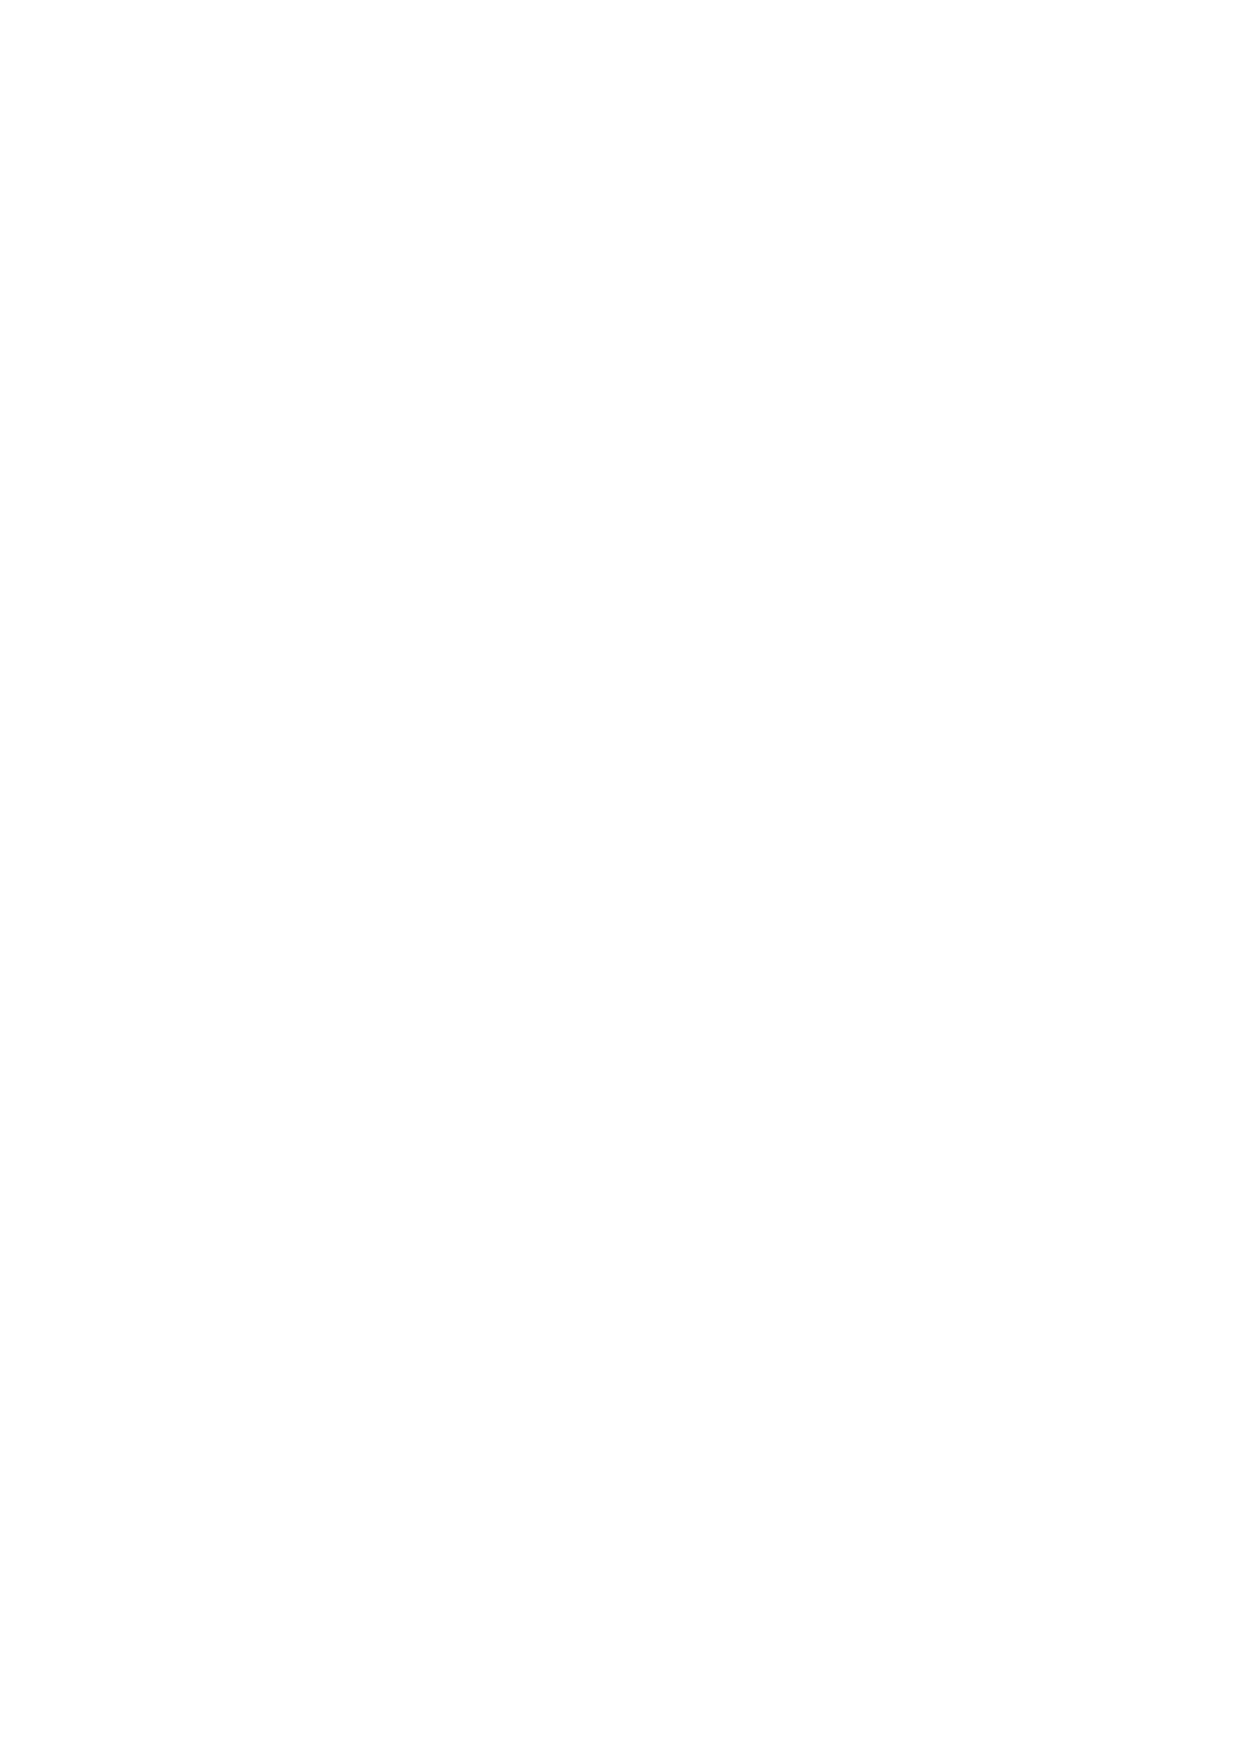
\includegraphics[width = 0.45\textwidth]{unihei_logo_bl}\\[1cm] % Include a department/university logo - this will require the graphicx package
%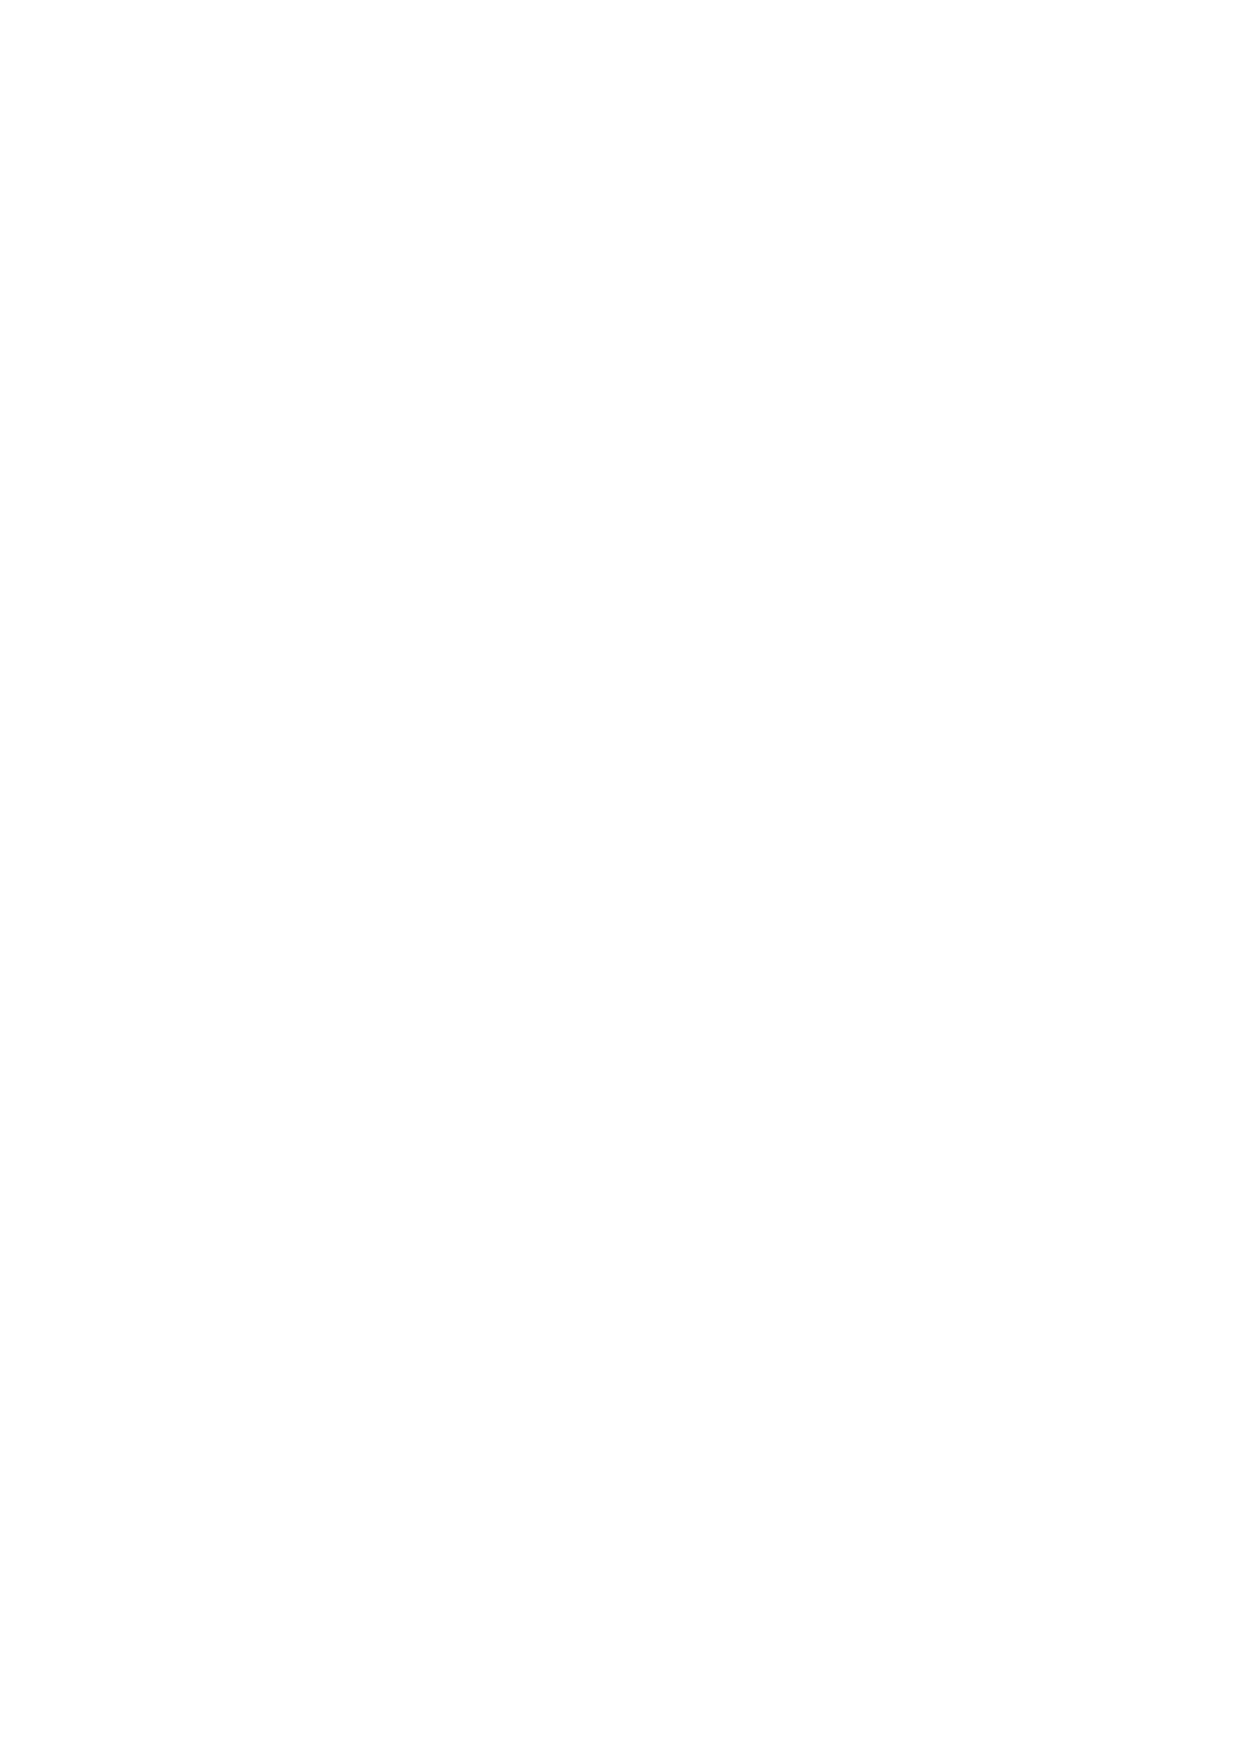
\includegraphics{unihei_logo_bl}\\[1cm] % Include a department/university logo - this will require the graphicx package
 
%----------------------------------------------------------------------------------------

\vfill % Fill the rest of the page with whitespace

\end{titlepage} 
\newpage
\tableofcontents
\newpage
%

\section{Organisation}

\subsection{Distribution of Tasks}
In the following the task distribution is shown. If the section is mentioned, the subsections are composed by the same person, otherwise the subsections are listed separately.

\begin{table}[htb]\label{tab: tasks}
%\caption{The distribution of tasks and sections written by each team member.}
\begin{tabular}{p{2.8cm}p{8.3cm}}
Dennis Aumiller & length estimation (Intro and Method D)\\[1em]
Lina Gundelwein & team leader, filtering, thinning, nucleosome detection, angle measurements, assembling report\\
&Sections \ref{sec:Thinning}, \ref{sec:Nucleosome Detection}, \ref{sec:Angle Measurement}\\[1em]
Philip Hausner& \\[1em]
Philipp Jung &  software architecture, performance optimization\\
&Section \ref{sec:Software Architecture}, \ref{sec: Adaptive Thresholding}, \ref{sec: Level Background}, \ref{sec: Outlier Removal}, \ref{sec: Limit Threshold}\\[1em]
Susanne Ibing & literature research, test data creation, validation, assembling presentation slides\\
& Section \ref{sec: Related Work}\\[1em]
Sarah Schott & literature research, test data creation, validation\\
& Section \ref{sec: Related Work}\\[1em]
Christian Schütz& OpenCV denoising, thresholding (investigation of Octave functions), length estimation (Intro and Method C), evaluation tools\\[1em]
& Section \ref{sec:Denoising}, \ref{sec:Thresholding}, \ref{sec:bfs_ssp_length_estimation}, \ref{sec:PixelRecovery}\\[1em]
Roman Spilger& literature research, test data creation, validation\\[1em]
Oskar Staufer & literature research, test data creation \\
& Sections \ref{sec: AFM}, \ref{sec: Epigenetics and Histones}, \ref{sec: Histone Complexes by AFM} \\[1em]
Martin Würtz & team leader, literature research, test data creation, validation, assembling presentation slides\\
&Section \ref{sec:Test Data Creation}\\
\end{tabular}
\end{table}

\subsection{Time Schedule}
 In the beginning of the project, an expected time line was generated and presented. Now after finishing the project, it is possible to compare the expected and actual needed time for each subsection of the project (see Figure \ref{fig: timeline}. 
For most of the subsections, such as the project selection, team building, software architecture, generation of test data, optimization of the algorithm, protocol writing and the generation of the endpresentation, the expected amount of time is similar to the actual amount of time. Those subsections are mostly not dependend upon other previous tasks. 
For the implementation of the algorithm however, four more weeks were necessary. Many of the images were hard to work with since the background is often very noisy and sometimes include dirt or undefined particles. Due to the fact that we did not have a limitless amount of images, we were dedicated to try to make the algorithm a very robust one. As visible in Figure \ref{fig: timeline}, the filtering, denoising and thresholding of the images was very time consuming even though now very successful. For the next steps of the algorithm, a robust binary image was necessary which is why it took much longer than expected. 
The evaluation of the algorithms, test data and the biological results could only be performed after the successful establishing of the algorithm. Because of the delay in algorithm implementation, the evaluation took place as well four weeks later than expected. 
In general, Figure \ref{fig: timeline} shows that with the number of team members, effective, simultaneous working was possible during the project. 
\begin{figure}[htb]
\begin{center}
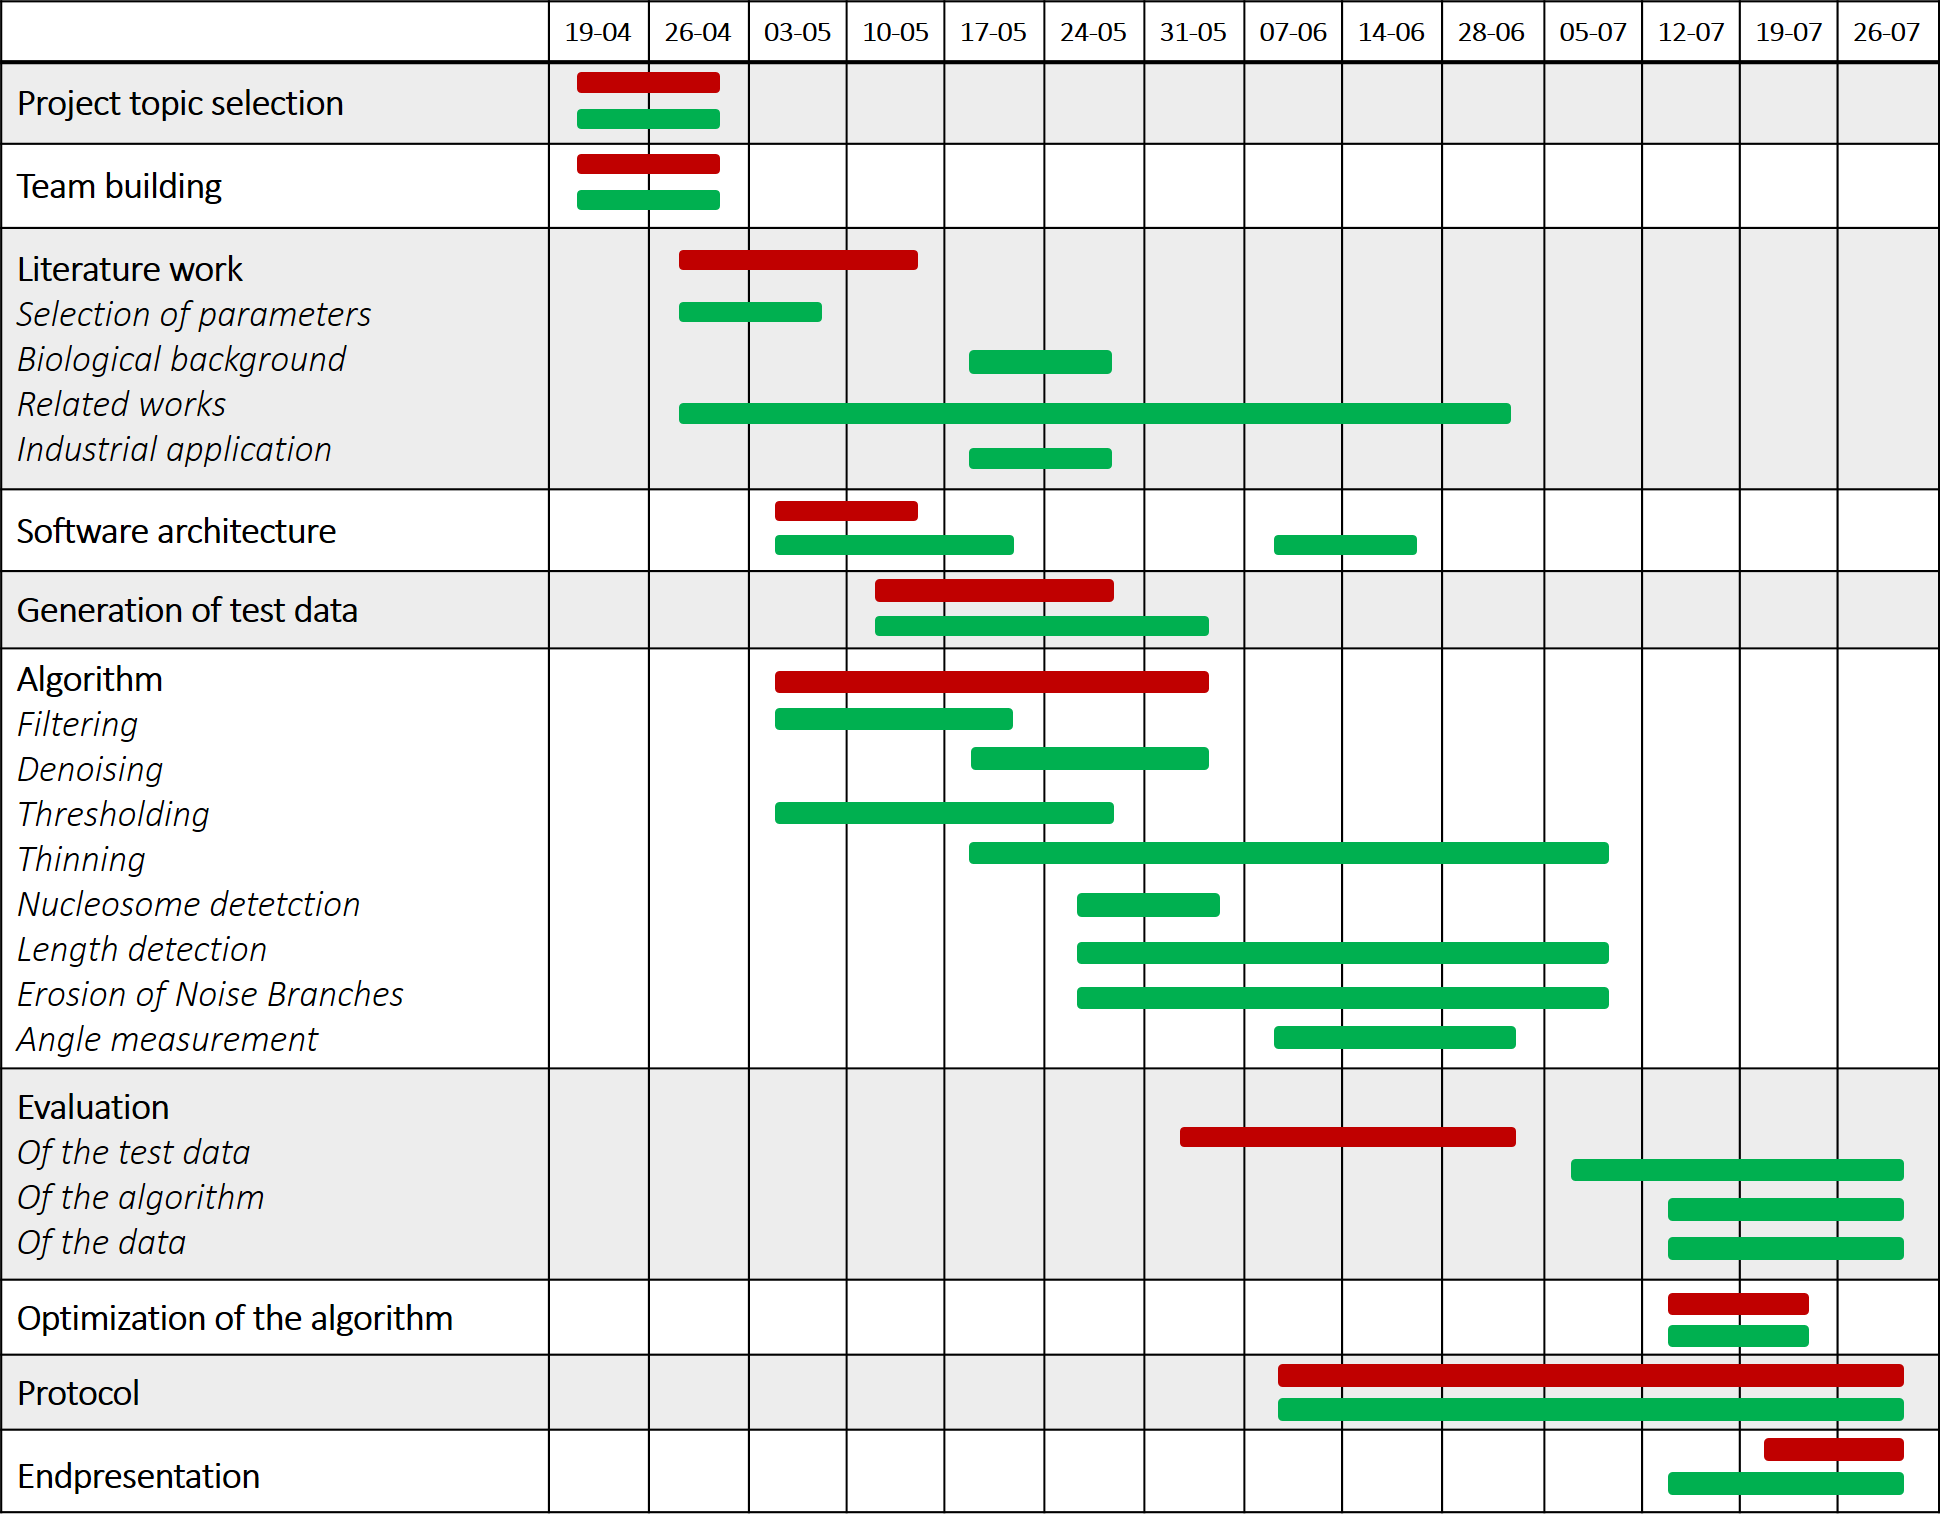
\includegraphics[width = \textwidth]{timeline2.png}
\end{center}
\caption{The expected needed amount of time for each subsection (red) and the actual needed amount of time (green).}
\label{fig: timeline} 
\end{figure}

\begin{abstract}
This report summarizes ...

\end{abstract}

\section{Introduction}\label{sec: Introduction}
\subsection{Motivation}\label{sec: Motivation}


\subsection{AFM}\label{sec: AFM}
Since its invention in 1982 by IBM scientists Gerd Binning and Heinrich Rohrer, atomic force microscopy (AFM) has found widespread applications in various fields ranging from semiconductor science to polymer physics. The simplicity of the underlying concept allows for implementation in a variety of challenging experimental setups including high-energy physics  \cite{fischbach2001new} and live cell biology  \cite{evans2007forces}. The AFM technology has particularly been used not only to obtain high-resolution topographic images (with resolution of up to 1 nm) but also to measure extremely low forces that occur for example during molecular interactions. In this way, major achievements, like first topologies of single atoms and small molecules and their connecting electron bonds, have been made possible  \cite{hoffmann2001direct}.As AFM is a non- destructive imaging technique and large fields of view can be scanned on appropriate time scales, it has found more and more application in the study of living cells and organisms (Figure \ref{fig: phage genome}). Here, it enables even for high resolution studies of the interactions between single cell membrane receptors and ligand drugs \cite{willemsen2000biomolecular}. Moreover, as nanotechnological approaches are becoming increasingly popular, AFM has gained attention for quality control purposes in industry and academia. 

However, automated evaluation of AFM images has remained challenging, especially when highly diverse biological structures, such as DNA molecules, are studied. Mostly because high background and varying morphologies hinder accurate automated evaluations. We here present an image processing algorithm, designed for automated quantification of AFM data to further study DNA histone interactions in higher throughput. 

\begin{figure}[htb]
\centering
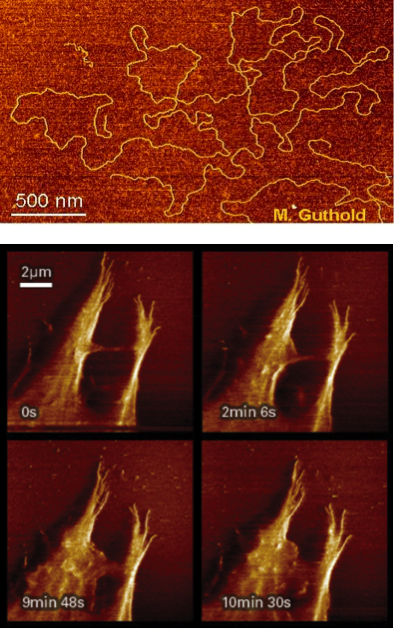
\includegraphics[width = 0.5\textwidth]{Figure1}
\caption{(Top) AFM image of a complete $\lambda$ phage genome with single strand resolution. Colors represent cantilever tip deflection \cite{image11}. (Bottom) AFM image of a living cell showing filopodia rearrangement. Colors represent cantilever tip deflection \cite{image12}.}\label{fig: phage genome}
\end{figure}

\subsubsection{Concept}
The heart of an AFM setup consists of a sharp silicon tip with an ending radius of curvature of up to 1 nm attached to a flexible micro cantilever (Figure \ref{fig: afm setup}). 

\begin{figure}[htb!]
\centering
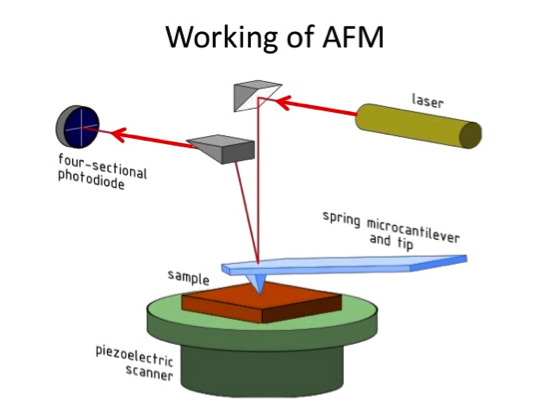
\includegraphics[width = 0.75\textwidth]{Figure2}
\caption{Schematic representation of an AFM setup with optical path of the laser beam in red and xy-controllable Piezo scanner \cite{image2}.} \label{fig: afm setup}
\end{figure}

The cantilever is mounted onto a Piezo controlled z-stage for precise lifting and dipping. With this, the cantilever tip is brought into (close) contact to the surface to be examined. The tip is then further scanned over the surface with constant z-stage deflection and thereby bended by topographic heterogeneities of the sample according to the mechanics described by Hook for simple springs. To precisely measure and amplify these minimal deflections, a focused laser beam is projected onto the cantilevers reflecting top. Redirected onto a four photodiode detector, x- and y- deflection of the elastic cantilever can be recorded as potential differences between pairing photodiodes. Small bendings are thereby amplified by the laser deflection and can be used to compute topographic images. Although being extremely simple, high resolutions can be achieved that are mostly limited by the tips radius and shape (Figure \ref{fig: atom resolution}).

\begin{figure}[htb!]
\centering
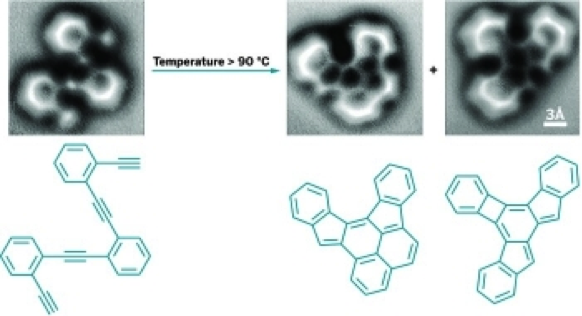
\includegraphics[width = 0.9\textwidth]{Figure3}
\caption{Single atom resolution AFM image and corresponding structural formula of an enediyne compound before and after induction of cyclisation by heating \cite{image3}.}\label{fig: atom resolution}
\end{figure}

However, to preserve the integrity of the examined specimens, which is of particular importance when observing living systems where harsh perturbations are likely to cause artifacts, the AFM is run in a so called tapping mode \cite{binnig1986atomic}. Here, an alternating current is applied to the supporting Piezo element thus oscillating the cantilever over the surface. By this, the tip-surface interaction is minimized and sample can be scanned with less interference.  
The core setup has been further modified and extended to even measure intermolecular forces \cite{hinterdorfer2006detection}. For this, the cantilever tip is slowly approached to a surface. At a specific distance, electrostatic forces will lead to an attraction of the tip and thus a bending of the cantilever. The kinetics of this bending are characteristic for differing molecular interactions \cite{cappella1999force}. By attaching molecules of interest to the AFM tip, specific interaction between these and molecules located at a surface can be measured. Using this concept, the interplay between drug molecules and G-protein-coupled receptors on cell surfaces could be quantified \cite{radmacher1997measuring}. Furthermore, by using conductive tips, the electric properties of materials were studied, an approach that has found wide applications in semiconductor and microprocessor science \cite{lang2004conducting}. 

%Noteworthy, AFM is a non-optical imaging technique that records topographic features of surfaces and not their optical properties. Intensities depicted in AFM images thus correspond to height values (in commonly used TIFF formats scaled between 0-255) rather then photon counts, as in most other microscopy images. Furthermore, image contrast corresponds to surface topography gradients and not to optical density, photon phase drifts or fluorophore emission gradients like in convention optical microscopy setups. 

\subsection{Epigenetics and Histones}\label{sec: Epigenetics and Histones}
Genetic information is mostly encoded within the DNA sequence and its modular components known as genes. However, during the last decades epigenetic mechanisms that regulate genetic information processing, have been recognized as key players in gene regulation. To date, several mechanisms of epigenetic regulation have been found in eukaryotic cells \cite{bird2007perceptions}. Two of the most prominent examples are DNA methylation and chromatin rearrangement.  While methylation is a direct chemical modification of DNA that leads to impaired recognition by DNA interacting proteins \cite{cuozzo2007dna}, chromatin remodeling mechanisms are versatile \cite{jenuwein1998set,gottschalk2009poly,lin2007role}. Here, the accessibility of specific sequences which are crucial for DNA processing are altered. The central elements of chromatin structures are large heteromeric protein complexes known as histones \cite{marino2005histone}. These highly alkaline proteins are exclusive to eukaryotic cells and some archaea, where they act as spools around which DNA can bind.  In this way, histones do not only alter DNA accessibility but also condense the genetic information within the nucleus, a critical steps especially during cell division. 

\subsubsection{Chromatin and Histone Structure}\label{sec: Chromatin and Histone Structure}
Histone complexes are formed between five major components, the histones proteins H1/H5, H2B, H2A, H3 and H4 \cite{marino2005histone}. The histone core is formed between H2A, H2B, H3 and H4 while H1/5 is known to serve as a linking element. The core histones exist as homodimers; all possessing a histone fold domain that is crucial for the interaction between the different dimers. This domain is comprised of three alpha helices that interact as handshake motifs with corresponding domains on the dimer partner. Thus, the histone complex is an octameric aggregate with an approximate diameter of 63 Å where 147 DNA base pairs can wrap around in 1,65-left handed turns. The histone protein H1 binds to the entering and exiting DNA strand thereby stabilizing the DNA histone complex. H1 is also crucial for the formation of higher order chromatin complexes as it mediates the arrangement of histone fibers in which several histone-DNA complexes pair to highly condensed chromatin (Figure \ref{fig: chromatin structure}). 

\begin{figure}[htb]
\centering
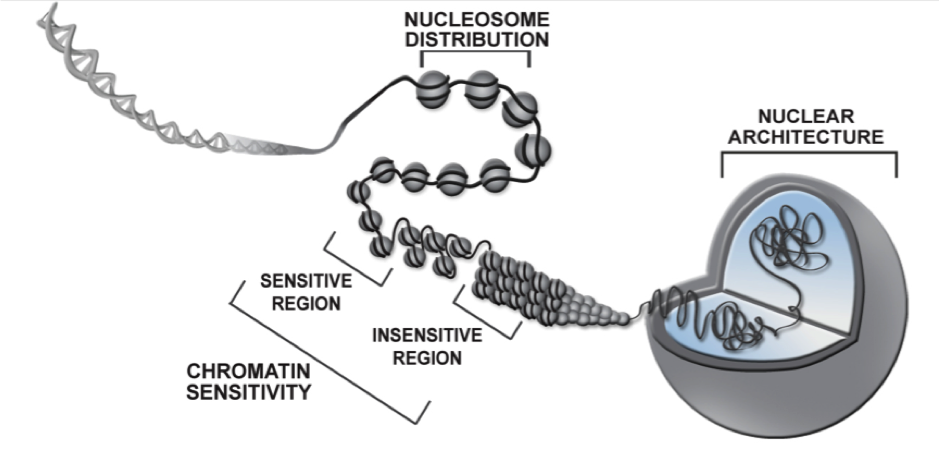
\includegraphics[width = 0.9\textwidth]{Figure4}
\caption{Chromatin structure from a single DNA double helix (left) to the fully evolved nuclear DNA architecture (right). DNA bound single histones are depicted in their modification sensitive conformation, where epigenetic mechanisms regulate gene transcription, and their insensitive condensed form \cite{image3}. }\label{fig: chromatin structure}
\end{figure}

\subsubsection{Histone Modifications}\label{sec: Histone Modifications}
Together with DNA methylation, chemical modifications of histone complexes are a key process in epigenetic regulation as with this, interactions between DNA and nuclear proteins such as transcription factors, polymerases or other regulatory elements can be altered \cite{mersfelder2006tale}. As histones represent complex macromolecular structures, the possible chemical modifications are diverse and yet not fully understood. However, some key players have been identified. Most modifications occur at the tails of histone proteins H3 and H4, which protrude from the DNA-histone complex \cite{lorch1987nucleosomes} (Figure \ref{fig: crystal structure}). 

\begin{figure}[htb]
\centering
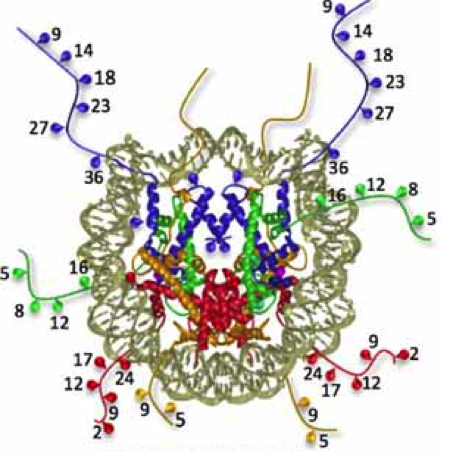
\includegraphics[width = 0.5\textwidth]{Figure5}
\caption{Crystal structure of a histone complex with a modeled double helical DNA strand wrapped around. Colors represent histone dimers (H2A yellow, H2B red, H3 blue, H4 green). Numbers correspond to amino acid sequence position and show frequent modification sites \cite{hansen2010histone}. }\label{fig: crystal structure}
\end{figure}

Here, acetylations, methylations, phosphorylations, ubiquitinations and citrullination have been reported. Additionally, the histone core can also be modified leading to highly complex modification patterns as several modification combinations can occur. By this, either the direct interaction between the DNA and a histone is sterically hampered or the modification acts as a recognition element for other regulatory proteins. For example, lysine acetylation in histone complexes is responsible for the loss of one positive charge and therefore reduces the electrostatic interaction strength to the negatively charged DNA backbone \cite{ozdemir2005characterization}. Therefore, acetylated histones are thought to form less condensed and thus more accessible chromatin structures. On the other hand, gene promoter regions that are bound to non-acetylated histones are known to be responsible for gene down regulation. Another prominent example for histone modification is lysine methylation. Here, up to three methyl groups can be added to a lysine residue at the histone tail. Although this does not diminish the positive lysine charge and thus no direct inhibition of the DNA-histone complex formation is observed (even if the small methyl groups slightly sterically alter this interaction), it serves as a recognition motive for other nuclear responsive elements with Tudor or PHD domains \cite{schotta2004silencing}. The underlying mechanisms appear to be extremely sensitive, as opposite effect between mono- and demethylation have been reported \cite{kourmouli2004heterochromatin}. 
Some well-studied histone modifications that promote gene transcription are triple methylation of H3 lysine 4, which mostly occurs in the promoter region of highly transcribed genes \cite{krogan2003paf1}, and triple methylation of H3 lysine 36, which is frequently observed in the gene bodies of upregulated genes as it recruits histone deacetylase thereby ensuring proper gene transcription \cite{strahl2002set2}. Prominent examples for modifications that repress gene transcription are trimethylation at lysine 27 of H3 \cite{cao2002role}, which induced histone acetylation, and trimethylation of H4 lysine 20 \cite{schotta2004silencing}. 
Hence, histone modification is a generally accepted epigenetic mechanism to regulate gene transcription, where the interaction strength between histones and DNA is of major importance. Mutations within histone complexes that alter this interaction have been associated with various diseases like cancer and chronic inflammations \cite{sawan2010histone}. 

\subsection{Histone Complexes by AFM}\label{sec: Histone Complexes by AFM}
As DNA-histone configuration is of major importance for epigenetic regulation, a profound understanding of the regulatory mechanisms and crucial structural features that conquer this interaction is highly desirable and of special interest for drug design. Here, the AFM technology is preferentially suited to study the molecular configuration with sufficient resolution. AFM is not only able to easily resolve single DNA strands but also to image the volume of single DNA-histone complexes (and thereby the number of DNA turns per histone) and the entering/ exiting angle of bound DNA, which gives insides into the bonding strength between DNA and histone. 
An automated evaluation of DNA structure is not only of interest to study DNA-protein interaction but also to evaluate cancerogenic compounds that alter the DNA architecture. Here, correlations between the cancerogenicity and the geometrical deformation of the compound bound DNA have been observed \cite{japaridze2015influence}. Therefore, quantitative screening of pharmaceutical compounds for their ability to influence DNA structure with AFM resolution could be highly interesting for toxicity studies. 
Moreover, many modern technologies used within the life science sector are based on DNA molecules. For example DNA bound antibodies have been used for immunohistochemical stainings where a DNA bound fluorophore enhances the fluorescence signal \cite{chen2015expansion}. Other applications include DNA micro arrays to study and compare gene expression \cite{adomas2008comparative}. Here, DNA molecules with specific gene complementary sequences are spot printed onto glass cover slips to quantify the amount of specific cDNA present in probes. This widely used technique can monitor slight changes in gene expression. However, quality control of the microarrays themselves has remained challenging. Specialized ventures already test for DNA microarray quality by AFM imaging but are yet not able to provide single DNA strand resolution as automated evaluation of this has been elusive \cite{dokukin2011towards}. With the here presented algorithm we tackle current restrictions in DNA-protein interaction analysis and DNA morphology quantification by AFM. 
\subsection{Related Work}\label{sec: Related Work}
The analysis of AFM images can be categorized into manual, semi-automatic and automatic approaches. Since manual image analysis were human operators draw manually the backbone of DNA filaments is very time consuming and error-prone, we focused on a fully automatic analysis without any supervision. In semi-automatic image analysis approaches, the threshold had been set manually or the initial and/or final point of a DNA filament was set by a human operator  \cite{wiggins2006high},  \cite{marek2005interactive},  \cite{cassina2016effects}.

Automatic image analysis predominantly focussed on the determination of the contour length of DNA filaments  \cite{spisz1998automated},  \cite{sanchez2002accuracy},  \cite{sundstrom2012image},  \cite{marturelliautomated}. The steps of the algorithms are very similar and will be explained below. The contour length is defined as the polymer’s length at maximal physical extension  \cite{rivetti2001accurate}.  Some research groups also considered the curvature or the spatial orientation of DNA filaments  \cite{ficarra2005automated},  \cite{ficarra2005automatic}. 
Doyen et al. used an automated approach for nucleosome recognition according area and height criteria and free DNA length determination of the nucleosomes.

The main steps of DNA contour length determination are first the generation of a binary image, then the skeletonization of traced DNA fragments, and then the length measurement. Many papers are referring to additional optional steps which are not necessary depending on which algorithms were implemented for the thinning step. In the following sections the single steps of the algorithms are explained. 
\subsubsection{Filtering}
In order to reduce the noise, one apply filters before generating the binary image. The filters are either 3x3 mean filters  \cite{rigotti2005quantitative} or 3x3 median filters  \cite{ficarra2005automatic},  \cite{ficarra2002automated} or a Gaussian filter and an adaptive filter  \cite{ficarra2005automated}. 

\subsubsection{Segmentation}
The generation of a binary image is based on a thresholding algorithm which is either determining the threshold globally or locally, depending on the method. Global thresholds are only considering the individual grey value of a pixel, whereas in local thresholding, the neighbourhood of a pixel is critical as well  \cite{weszka1978survey}. A neighbourhood of a pixel consists of four or eight pixels. They can be included in the thresholding process by calculating the mean or median of the grey values. Since local thresholding methods are very CPU-intensive, most studies use global thresholding algorithms. Their thresholds mostly depend on the pixels’ intensity values, whereas in one case a global threshold of 0.2 nm was used  \cite{sanchez2002accuracy}. Finding the optimal threshold, where only valid fragments and no background are considered, is a challenging task. Ficarra et al. \cite{ficarra2005automated}, \cite{ficarra2005automatic}, \cite{ficarra2002automated} use the Ridler method \cite{ridler1978picture}, a method based on a grey value histogram which iteratively determines the optimal threshold. Spisz et al. \cite{spisz1998automated} use two different thresholding techniques. The first technique is based on two Gaussian distributions fitted to the fore- and background grey values and finds the optimal threshold in between those distributions  \cite{gonzales1987wintz}. The algorithm cannot be applied to all AFM images, therefore they implemented a second method which finds the minimum threshold where the number of recognized fragments (blobs) does not change  \cite{russ1992image}. Setting a too high threshold leads to the fragmentation of DNA filaments (see Figure \ref{fig: blobs}).

\begin{figure}[htb]
\begin{center}
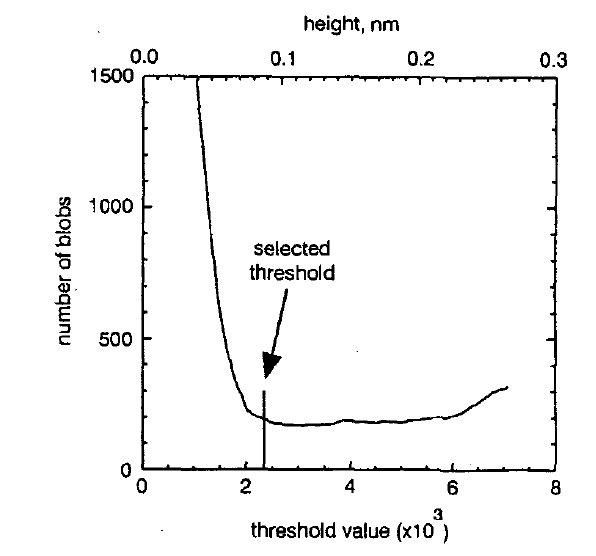
\includegraphics[width = 0.7\textwidth]{Segmentation_histo}
\end{center}
\caption{Determination of an optimal threshold. For each threshold the resulting number of blobs were calculated. The optimal threshold is the minimal threshold value at which the number of blobs does not decrease any further. \cite{russ1992image}}
\label{fig: blobs} % you need to include this to reference the figure afterwards
\end{figure}

Another option is to consider a pixel’s neighbouring intensity values instead of the pixel’s intensity value  \cite{marek2005interactive}. By doing so, filtering and segmentation are combined into one step.


\subsubsection{Thinning}
The thinning step is used in order to erode the fragments to skeletons with the width of one pixel which is necessary for the length determination. The fast parallel thinning algorithm by Zhang and Suen iteratively removes pixels from each fragment if they possess all the conditions of removal  \cite{ficarra2005automated},  \cite{ficarra2002automated},  \cite{ficarra2005automatic},  \cite{spisz1998automated},  \cite{zhang1984fast},  \cite{marturelliautomated}. This algorithm does not remove corner pixels and removes valid end pixels with a high probability. The algorithm by Brugal and Chassery \cite{brugal1977new},  \cite{sanchez2002accuracy} iteratively removes connected pixels in a specific order. The end pixels are not affected by the algorithm, therefore no end pixel restoring is necessary. Sundstrom et al. do not describe their thinning algorithm but only emphasize that it is necessary to convert the fragments into skeletons with a width of one pixel  \cite{sundstrom2012image}.


\subsubsection{Removal of Corner Pixel}

During thinning invalid corner pixels can be included into the DNA skeleton which results in a longer distance in corner areas. Those pixels are not real compartments of the DNA structure and hence need to be removed  \cite{sanchez2002accuracy},  \cite{ficarra2002automated},  \cite{spisz1998automated}.

\subsubsection{Removal of Objects Across the Image Boundary}

For fragments at the image boundary a complete analysis is not possible. Therefore, such fragments have to be excluded from further steps. Ficarra et al. used a 8-pixel neighbourhood for the detection of such objects. If the connectivity in the neighbourhood was not interrupted at the image boundary the object has been removed  \cite{ficarra2005automated},  \cite{ficarra2005automatic}. 

\subsubsection{Pruning}

After thinning some short branches often remain at the skeletons. The reasons are impurities in the sample or noise close to the DNA fragment. Sundstrom et al. \cite{sundstrom2012image} referred to a master thesis by Silvio Cirrone CHECK who transformed the skeleton into a graph. Thus the problem was formulated as a graph optimization problem to cope with short branches. Otherwise, the removal of the branch pixels is necessary. Ficarra et al. \cite{ficarra2002automated},  \cite{ficarra2005automated} created a mask to distinguish between unbranched and completely detected cases, branches, critical cases, and corners. Spurious branches have the characteristic of being much shorter than the fragment. This feature is used to identify such branches and to delete them recursively.  



\subsubsection{Removal of Invalid Fragments}

In this step, critical molecules are removed before analysing their length. Spisz et al. \cite{spisz1998automated} carry out this step before thinning the fragments. Fragments are defined as invalid when they are overlapping with other fragments or with themselves, when they are in a closed circle conformation, when the endpoints are not distinguishable, when more than two endpoints are detected and when they exceed a user-defined size  \cite{spisz1998automated},  \cite{ficarra2005automated},  \cite{ficarra2002automated},  \cite{ficarra2005automatic}. Ficarra et al. used for the removal of such invalid fragments different masks. For overlapping molecules the masks shown in Figure \ref{fig: Masken} have been used  \cite{ficarra2005automated}.

\begin{figure}[htb]
\begin{center}
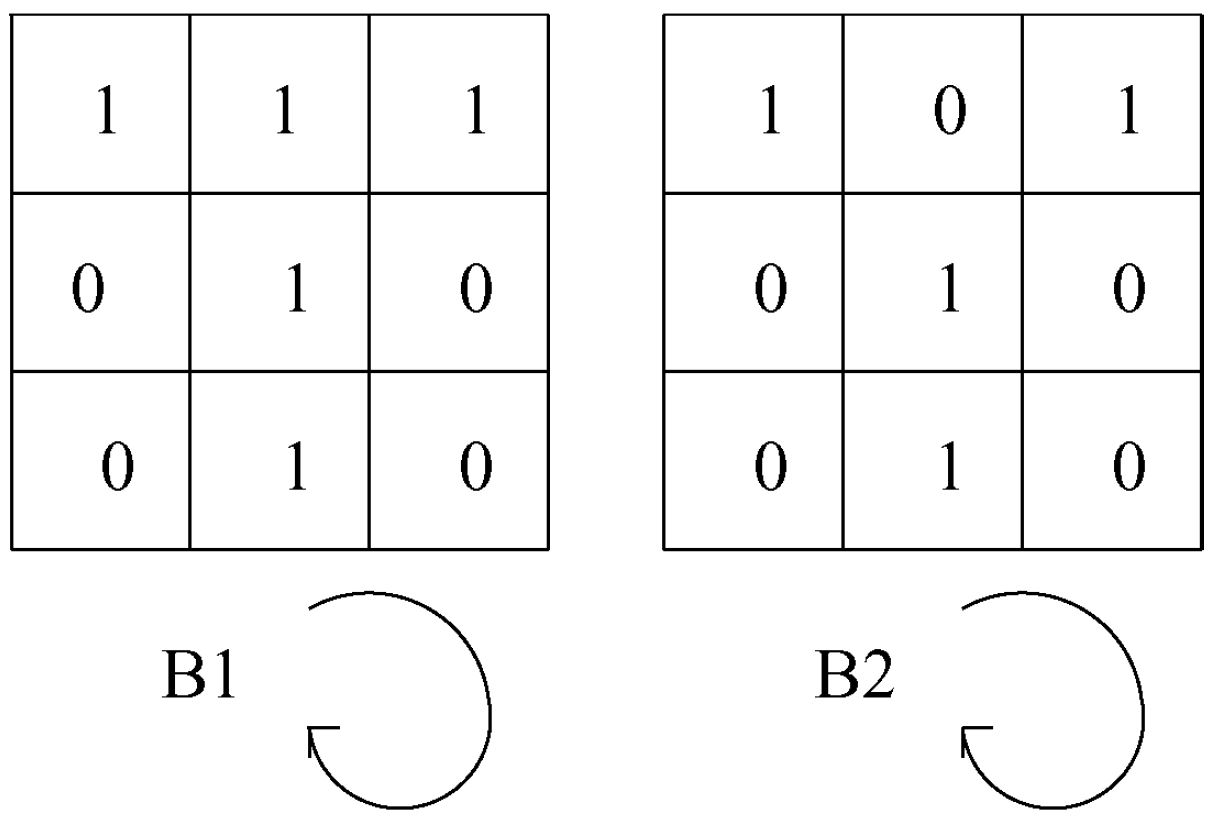
\includegraphics[width = 0.7\textwidth]{Masken}
\end{center}
\caption{Masks for identifying overlapping molecules. \cite{ficarra2002automated}}
\label{fig: Masken} % you need to include this to reference the figure afterwards
\end{figure}



\subsubsection{Pixel Restoring}\label{sec:IntroPixelRestoring}

Pixel at the skeleton ends only need to be restored if they were erroneously deleted during thinning of the fragment. The end pixels of each backbone are virtually extended in the direction of the last two pixels. If the new possible end point was part of the fragment before, the pixel is restored  \cite{spisz1998automated},  \cite{ficarra2005automated},  \cite{ficarra2002automated},  \cite{ficarra2005automatic}.



\subsubsection{Length Determination} \label{intro_length_determination}

The determination of the length of the DNA skeletons is achieved by estimating the contour length which is defined as the polymer’s length at maximal physical extension  \cite{rivetti2001accurate}.  During digitization, the exact contour is lost. Anyhow, the accurate determination of the contour length is for many applications crucial. The Freeman estimator is the most commonly used method to determine the length  \cite{spisz1998automated},  \cite{marturelliautomated}. When the fragment is reduced to a skeleton with the width of one pixel, the connection between one and another pixel can be represented by eight directions (Figure \ref{fig: freeman}A). The Freeman estimator is adding the distance between the connected pixels from one endpoint to another. Even connections thus with vertical or horizontal direction are counting as 1, odd connections with diagonal connections are multiplied by 1.414. \\

$ L_{F} = n_{e} + \sqrt{2} n_{o}= 1.000n_{e} + 1.414n_{o}  $ 

\hspace{0,2cm}
 
$ L_{F}$: \begin{footnotesize} 
DNA contour length determined by the Freeman estimator
\end{footnotesize}  

$ n_{e}$: \begin{footnotesize} 
 number of even connections
\end{footnotesize} 
 
$ n_{o}$: \begin{footnotesize} 
 number of odd connections
\end{footnotesize}  \\

Even though the Freeman estimator is often used, it overestimates the DNA length by approximately eight percent  \cite{sanchez2002accuracy}. Rivetti and Codeluppi \cite{rivetti2001accurate} analysed in 2001 six different algorithms to determine the contour length, one of them being the Freeman estimator. 
Secondly, they tested the most probable origin estimator, which similar to the Freeman estimator computes an ($n_{e}$, $n_{o}$) characterization. This algorithm calculates the contour length as a function of the number of egde pixels, number of pixels on diagonal edges and of the area \cite{pan1991root}, \cite{dorst1987length}. \\

$ L_{MPO} = \sqrt{(n_{e} + n_{o})^{2} + n_{e}^{2}} $

\hspace{0,2cm}

$ L_{MPO} $: \begin{footnotesize}
DNA contour length determined by the most probable origin estimator
\end{footnotesize} \\

Much better results were obtained for the Kulpa estimator which is derived from the Freeman estimator. The coefficients of even and odd pixels minimize the error when measuring the length of long fragments.\\

$ L_{K} = 0.948n_{e} + 1.343 n_{o} $

\hspace{0,2cm}

$ L_{K} $: \begin{footnotesize}
DNA contour length determined by the Kulpa estimator
\end{footnotesize} \\

The corner count estimator considers additionally to the number of even and odd connections the number of different code pairs, so called corners (Figure \ref{fig: freeman}B)  \cite{vossepoel1982vector}. The coefficients were found by least-square fitting  \cite{yang1994methods}.  \\


$ L_{C} = 0.980n_{e} + 1.406 n_{o} - 0.091 n_{c} $

\hspace{0,2cm}

$ n_{c} $: \begin{footnotesize}
number of corners
\end{footnotesize} \\


\begin{figure}[htb]
\begin{center}
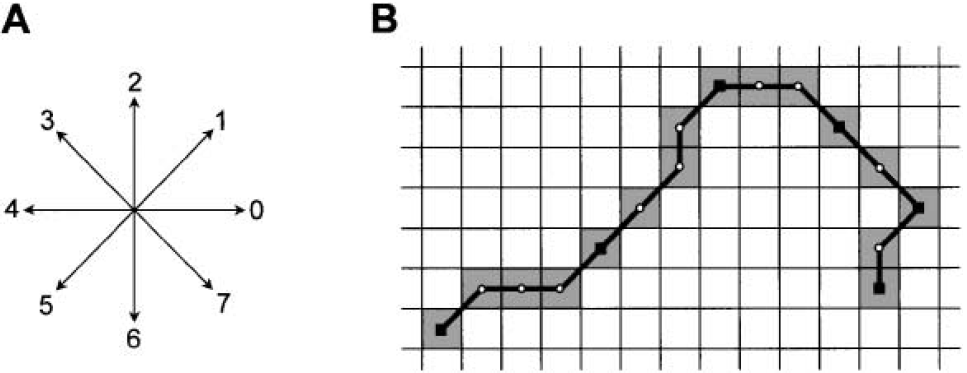
\includegraphics[width = 0.7\textwidth]{freeman}
\end{center}
\caption{(A) Scheme of the eight connected chain code. (B) Example of a fragment skeleton containing 16 pixels (grey grid elements). The chain is connected by 15 codes, from the left to the right chain the codes can be written as 100111210077756. There are six even codes ($ n_{e} $) and nine odd codes ($ n_{o} $). The total number of corners ($ n_{c}$) is six.}
\label{fig: freeman} % you need to include this to reference the figure afterwards
\end{figure}

As fourth estimator Rivetti and Codeluppi tested an estimator where the backbone was primarily smoothed by using polynomial fitting. The coordinates of each pixel where thereby adjusted. The polynomial degree was three and the moving window consisted of five points since the estimation with this combination were very close to the real length. \\ 

$ L_{PF} = \sum_{i=1}^{n-1} \sqrt{(x_{i+1}-x_{i})^{2} + (y_{i+1}-y_{i})^{2}} $

\hspace{0,2cm}

$ L_{PF} $: \begin{footnotesize}
DNA contour length determined with polynomial smoothing
\end{footnotesize} \\



The last algorithm included in their analysis was the edge chain algorithm which was originally implemented to measure the length of the roots of plants. It can be applied for other objects with relatively constant width and draws chords along the object edge to determine its perimeter. \\

$ L_{ECA}=\dfrac{P+\sqrt{P^{2}-16A}}{4} $

\hspace{0,2cm}

$ L_{ECA} $: \begin{footnotesize}
DNA contour length determined by the edge chain algorithm 
\end{footnotesize} 

$ P $:\begin{footnotesize}
perimeter
\end{footnotesize} 

$ A $:\begin{footnotesize}
area
\end{footnotesize} \\

Rivetti and Codeluppi generated synthetic data similar to their AFM images with DNA fragments of different length and tested the estimators while knowing the exact length of the synthetic filaments. The estimations with the Kulpa estimator, the corner count estimator, and with polynomial smoothing were significantly closer to the real length of the filaments than the estimates generated by the other three estimators. The overestimation of the Freeman estimator was confirmed  \cite{rivetti2001accurate}.



Ficarra et al. \cite{ficarra2002automated},  \cite{ficarra2005automated} calculated the molecule length using the Euclidean distance which was integrated over all consecutive pixels of the molecule. For calculation the pixel coordinates were recalculated as weighed average by using a weight factor k.\\


$ X_{P} = k(x_{p-1}-x_{p})+x_{p}+k(x_{p+1}-x_{p}) $

$ L_{P+1,p}= \sqrt{(X_{p+1}-X_{p})^{2}+(Y_{p+1}-Y_{p})^{2}} $

\hspace{0,2cm}

$ X_{P} $:\begin{footnotesize}
weighed average x coordinate
\end{footnotesize}

$ k $:\begin{footnotesize} 
single weight factor
\end{footnotesize}

$ L_{p+1,p} $:\begin{footnotesize} 
modified distance between the points with coordinates x and y
\end{footnotesize}\\




\section{Methods}\label{sec:Methods}
\subsection{Test Data Creation}\label{sec:Test Data Creation}
Missing: Description of the images we are using
\subsubsection{Manual Analysis}\label{sec:Manual Analysis}
To annotate and evaluate the results of the algorithm the open source program ImageJ (2.0.0-rc-46/1.50g) was used. Therefore, the features from a sample of objects or from whole images, were analyzed manually with the tools of ImageJ.
For the objects, which were single DNA-strands and mono nucleosomes, the location and the couture length were determined. For nucleosomes, also the angle between the two DNA-strands entering the nucleosome core, the approximate area of the nucleosome core and the mean gray value of the nucleosome core were measured.
To annotate the manual data from one object to the results of the algorithm the centre of mass was used. Therefore a binary image was created by thresholding. Then the "Analyze Particle Tool" was used to read out the x-y coordinates of the centre of mass from the different objects. 
All other parameters were determined on the original images. To measure the different lengths, the "Segmented Line Tool" was used. One end of a DNA strand was set as starting point, from which the line-points were drawn centrally through the fragment towards the other end of the fragment. This so called couture length was also measured for mono nucleosomes, by drawing centrally through the DNA and through the approximate center of the nucleosome core (figure). For mono nucleosomes, however two lengths were determined. The second length was the distance between the approximate center of the nucleosome core and the end of the shorter of the two entering DNA-strands.
The entry/exit DNA-strand angles of mono nucleosomes were measured by using the three point selection "Angle Tool" of ImageJ. Figure illustrates that the entry/exit DNA-strand angles can be determined in two different ways. In that context, $\alpha_1$ and $\alpha_2$ were measured on different mono nucleosomes for the test data evaluation.
$\alpha_1$ was measured by connecting the two entry/exit points of the nucleosome with the approximate center of the nucleosome core. For the determination of $\alpha_2$, the two DNA-axes at the nucleosome core were traced. The angle between the two DNA-axes was then measured at their intersection point.
The approximate area and mean gray value of nucleosomes were determined by manually fitting an elliptical structure to the nucleosome cores with the "Oval Selection Tool" of ImageJ.
Besides single DNA strands and mono nucleosomes, the locations of special objects were recorded. The special objects were intersecting DNA-fragments/nucleosomes, self-intersecting DNA-fragments/nucleosomes, objects on the edges of an image and undefined objects. To increase objectivity, test data were measured from four different persons.

\begin{figure}[h!]
\centering
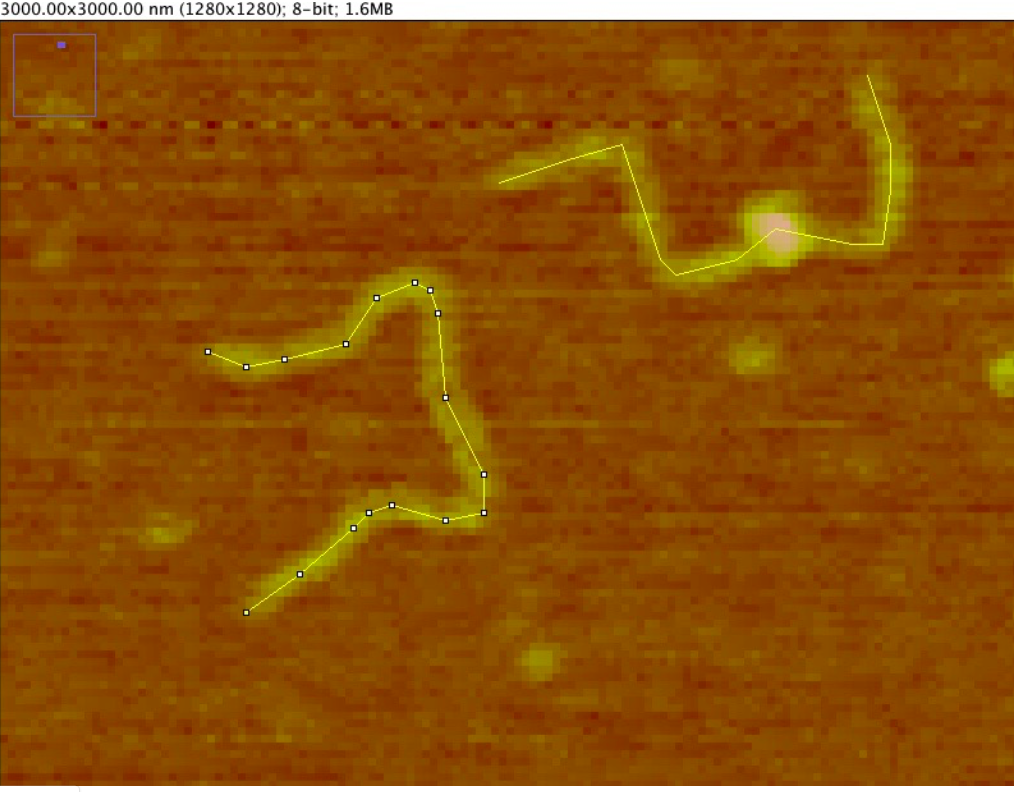
\includegraphics[width = 0.5\textwidth]{coutureLength.png}
\caption{Couture length measurements of DNA and nucleosomes
The contour length of DNA and nucleosomes were measured with the "Segmented line tool" of ImageJ. The white bars indicate the selected points. The lines have been traced centrally through the DNA fragments from one end point to the other end point.}
\label{fig: couture length}
\end{figure}

\begin{figure}[h!]
\centering
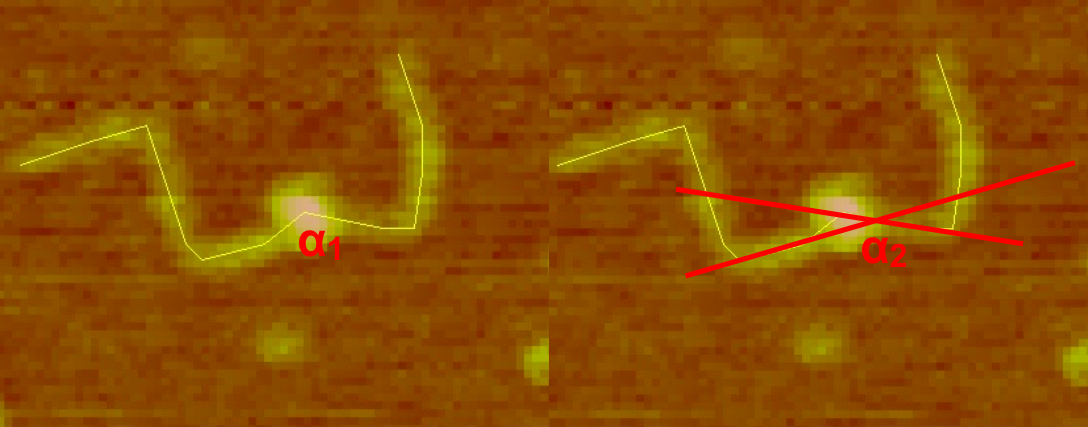
\includegraphics[width=0.7\textwidth]{angleMeasurement.png}
\caption{Angle measurement of mono nucleosomes
The figure shows two possible angles $\alpha_1, \alpha_2$ which can be measured between the two entering DNA strands of an nucleosome. $\alpha_1$ is the angle between the entry/exit points of the DNA with respect to the approximate center of the nucleosome core. $\alpha_2$ is the angle between the DNA-axes (red lines), which are crossing the entry/exit sites of the nucleosome core, with respect to their intersecting point.}
\label{fig: angle measurement}
\end{figure}
\newpage
\subsection{Software Architecture}\label{sec:Software Architecture}

\subsection{Denoising}\label{sec:Denoising}
The first steps in our MATLAB routine deal with preparing all images in order to binarize them with the most success, i.e. with the best DNA recognition rate as well as most accurate length estimation. This means that the routine removes as much noise and as many different kinds of noise so that it automatically and, before all else, correctly can classify any image pixel as either belonging to a DNA fragment / nucleus or as background.
For this to achieve, we found that the initial step needs to be a noise reduction method called \textit{Non-local Means Denoising}. It is very well suited to remove white noise from images, which is a noise type that is very typical for AFM images. White noise is defined as a random signal that has a constant power spectral density. Although the image processing library of MATLAB is very extensive, no function implementing \textit{Non-local Means Denoising} could be found. Those denoising functions that are provided by MATLAB, such as \textit{wdencmp} in conjunction with \textit{ddencmp}, or \textit{wiener2}, proved not to be as suitable for denoising the here analysed images, due to their very specific noise types (which are also discussed in greater detail in Sections \ref{sec:Filtering} and \ref{sec:Thresholding}). However, the method is provided by the open source computer vision and machine learning library \textit{OpenCV} (\cite{itseez2016opencvman} \cite{itseez2016opencvlib}). 

\subsubsection{Non-local Means Denoising Algorithm}
The algorithm of \textit{Non-local Means Denoising} is provided by the OpenCV library function \textit{fastNlMeansDenoising} that requires the following parameters:
\begin{itemize}
	\item \textit{filter strength} (float): The larger this parameter, the better noise is removed and the more details are lost. In our case we chose the value 2 since this appeared to provide a good balance between noise removal and loss of DNA details.
	\item \textit{template window size} (int): Window size in pixels of the patch that is used to compute weights. The recommended value is 7, which we found to be sufficient.
	\item \textit{search window size} (int): Window size in pixels of the patch that is used to compute the denoised value of the currently examined pixel from. Since this value affects performance linearly, we chose this value to be slightly smaller than the recommended value of 21, namely 17. This proved to be sufficient for good denoising results.
\end{itemize}
The heuristics to find these parameters were a) to achieve fastest possible runtime while b) providing satisfactory levels of denoising as measured by final DNA detection rate and length estimation accuracy. Increasing the search window size from 17 to up to 31 greatly increased the removal of background in the resulting preprocessed images. However, in conjunction with the subsequent steps of Filtering (\ref{sec:Filtering}) and Thresholding (\ref{sec:Thresholding}), this gain did not result in a notably improved detection rate of DNA objects or increased accuracy of length calculation (data not shown). Since it also had a drastic negative impact on the overall runtime, we decided to keep this parameter as low as possible without loosing the benefit of denoising. Comparable observations were made when investigating the required template window size. Increasing it resulted in increased runtime without any distinct gains in image denoising. \\

The great strength of this method is that for each pixel p of an image it searches for similar pixels - not in a close distance around that pixel, like many other noise reduction approaches do, but over a large portion of the image. The average value of these pixels is then calculated and set as the new, denoised value of the currently examined pixel p. In order to further increase robustness, similarity between two pixels p and q furthermore is computed by calculating a weighted Euclidean distance between square patches around these pixels, and not between only those two pixels. 
So, the denoised value $\hat{u}(p)$ of pixel p is calculated as follows:
\begin{center}
	$ \hat{u}(p) = \frac{1}{C(p)}\sum_{q \in B(p,r)}u(q)w(p,q) $
\end{center}
with
\begin{itemize}
	\item u(q) being the current value of pixel q
	\item B(p,r) being the  neighborhood of pixel p in a (2r+1) x (2r+1) large window centered at p
	\item C(p) being a normalisation factor:
	\begin{center} $ C(p) = \sum_{q \in B(p,r)} w(p,q) $ \end{center}
	\item w(p,q) being a weight function with an exponential kernel for the determination of similarity between pixels p and q:
	\begin{center}$ w(p,q) = e^{-\frac{max(d^2-2\sigma^2, 0.0)}{h^2}} $ \end{center}
	\item $d^2$ being the square Euclidean distance of the $(2f+1) x (2f+1)$ large color patches centered at p and q, respectively:
	\begin{center}
		$ d^2(B(p,f), B(q,f)) = \frac{1}{3(2f+1)^2}\sum_{j \in B(0,f)}(u(p+j)-u(q+j))^2$
	\end{center}
	\item $\sigma$ being the standard deviation of the noise
	\item h being a filtering parameter depending on the noise level $\sigma$
\end{itemize}
A much more detailed description of the algorithm can be found at \cite{ipol.2011.bcm_nlm}, which we recommend to the interested reader.

\subsubsection{Benefits of using Non-local Means Denoising}
As can be seen in Figure \ref{fig:denoising}, the denoising procedure results in a much sharper separation of DNA objects from their background than without. This is especially apparent when comparing the histogram of an yet unprocessed image with the histogram of the same image after it has been denoised (Figure \ref{fig:denoising_histograms}, upper row and lower row, respectively). Before denoising, all transitions between any at least slightly bright object and the background were rather smooth as is indicated by the overall brightness of the original image and the smooth surface of its histogram. However, after denoising, these transitions have become much steeper, which is represented by the gaps in the histogram of the denoised image and which is reflected in an increase of image contrast. Although not too strong in its distinctiveness, this outcome is the primary basis for the efficacy of all subsequent noise reduction measures.\\

Furthermore, some artifacts already could be removed. AFM images often show long but only few pixels wide horizontal lines that stem from the cantilever skipping while scanning the image. One such example is visibile in the upper image of Figure \ref{fig:denoising_imgs} in the lower left corner. This artifact is not visible anymore in the denoised image (lower image of Figure \ref{fig:denoising_imgs}) - it was replaced by background during denoising.

\begin{figure}[htb!]
	\centering
	\begin{subfigure}{0.28\textwidth}
		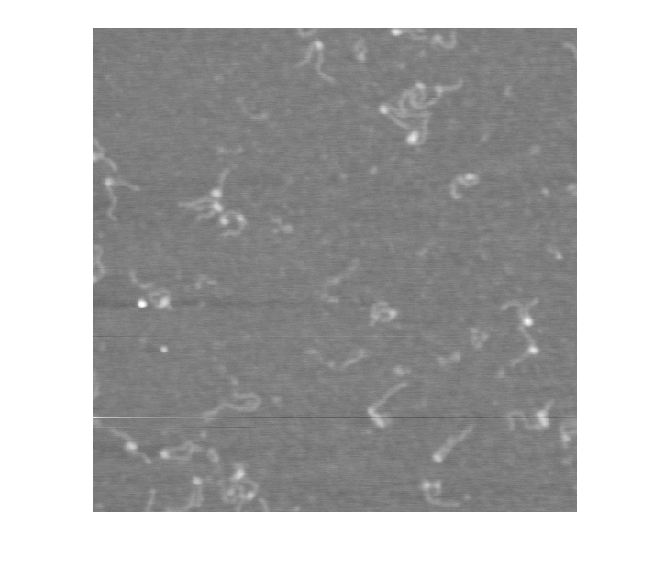
\includegraphics[width=\linewidth]{beforeDenoise_img.png}			
		
		\vspace{0.1cm}
		
		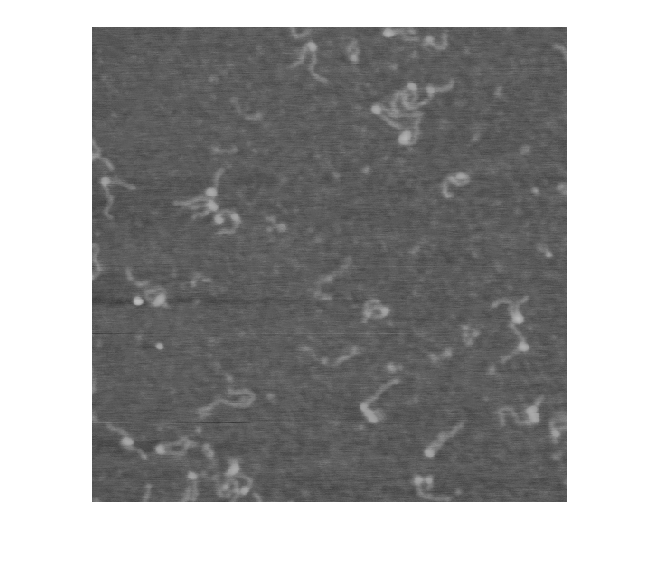
\includegraphics[width=\linewidth]{afterDenoise_img.png}
		\caption{}
		\label{fig:denoising_imgs}
	\end{subfigure}
	\begin{subfigure}{0.7\textwidth}
		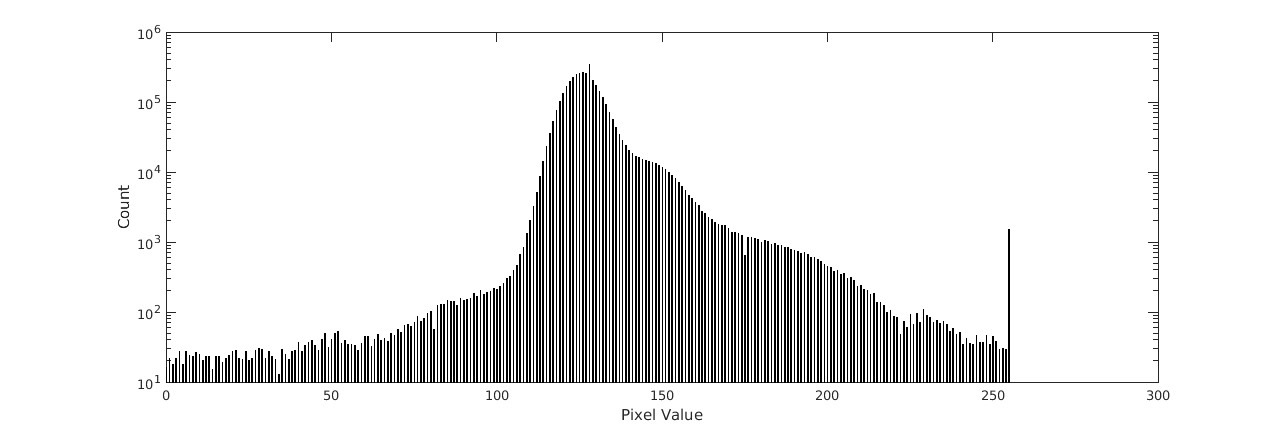
\includegraphics[width=\linewidth]{beforeDenoise_histogram.png}
		
		\vspace{0.1cm}
		
		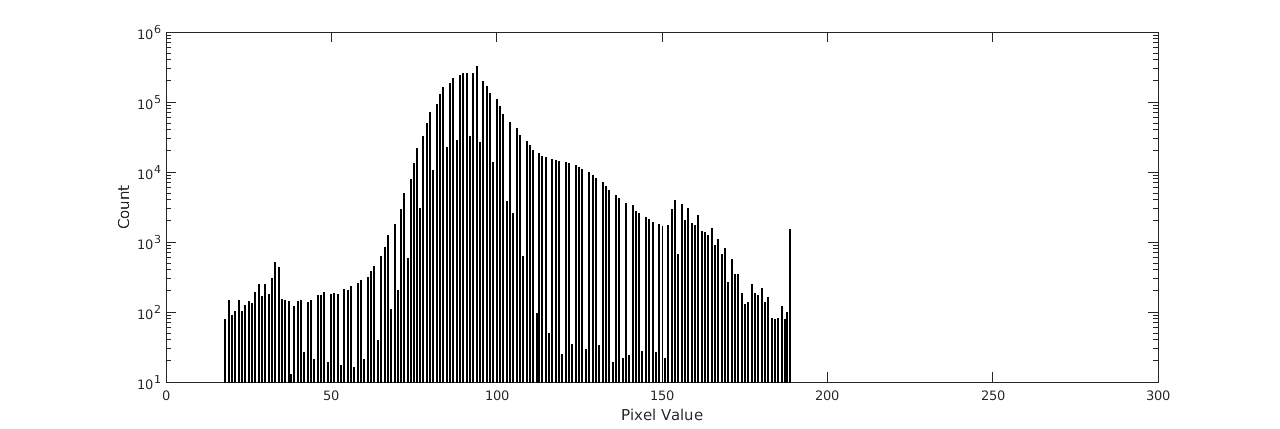
\includegraphics[width=\linewidth]{afterDenoise_histogram.png}
		\caption{}
		\label{fig:denoising_histograms}
	\end{subfigure}
	\caption{Effect of denoising procedure on grey scale images and their histograms.\\
		The upper row shows an unprocessed image before denoising (a) as well as its histogram (b), while the lower row shows the same image (a) and histogram (b) after denoising. Histograms show a logarithmic y-axis. It is apparent that denoising results in a sharper separation of DNA from background, thereby increasing the image's contrast.}
	\label{fig:denoising}
\end{figure}

\subsubsection{Technical considerations / limitations}
As mentioned in Section \ref{sec:Software Architecture}, our program is written using MATLAB. However, OpenCV is a C++ library, so \textit{fastNlMeansDenoising} is a C++ function. Consequently, we had to find a way to combine MATLAB with C++ code. \\
For such cases, there exists a C++ interface library that is provided by MATLAB (see \cite{opencvInterfaceSupport}). With its help, C++ code can be compiled into so-called mex files, which themselves call OpenCV functions and which can be called like regular MATLAB functions. We succeeded in integrating such specifically compiled mex files into our main program and, thusly, in denoising all images. Unfortunately, we had to discover that the resulting, denoised images were considerably different from those that had been denoised by the original C++ function. Since we were unable to discern the reason for this unexpected behavior, we had to find other measures to use OpenCV functionality from within our MATLAB routine. Therefore, our routine now makes a system call in order to run a C++ executable file. This file is a standard executable compiled from C++ code containing the denoising instructions; it will read all images, denoise them, and temporarily create and write new, denoised images. These images then are read by our MATLAB routine as input for the rest of the program.

\newpage
\subsection{Filtering}\label{sec:Filtering}
\subsubsection{Necessity of Filtering}
%Although it is common practice to use filtering techniques as a way of preprocessing the data, it was the goal 
At first, one needs to ask why it is necessary to use filtering techniques in the first place, as it is stated in various other papers (compare \cite{ficarra2005automated}, \cite{ficarra2005automated}). Since the goal of this work was to find a most efficient and fast solution, a heuristic approach was proposed which only took object size of connected components into account. For this the MATLAB function bwconncomp was applied to a black and white image of the thick DNA strands.\\
Although this eliminated most of the smaller fragments, and some larger ones, obviously some objects remained that were dirt or impulsive noise. \\
Like Ficarra et al. \cite{ficarra2005automated} pointed out, a median filter with a 3x3 mask helps eliminating these components quite well, yet there is still room for improvement. Regarding the aspect of very limited available data, it was another aim to maximize the number of sampled strings. Therefore, other, less common techniques besides the already tested filters were investigated.\\
As it was rather soon apparent that regions with impulsive noise had a rather high frequency, a lowpass filter approach seemed suitable.

\subsubsection{The Concept of Adaptive Low Pass Filtering}
Firstly, the most prominent example for a lowpass filter is the Gaussian filter. It essentially smoothes the data, but in a relatively predictive way, since it has a predefined filtering matrix. But, since the signal-to-noise ratio is not always known , a simple Gaussian filter might only blur the edges of the outer DNA regions, instead of effectively reducing the amount of white noise. Rather than simply smoothing the image with a Gaussian filter, the idea was to eliminate regions with high contrast.  \\
Removing such high-contrast regions is best achieved in frequency space. The freuquency domain, simply put, transforms the original image data into a decomposition of sinus waves. For the transformation between spatial domain and frequency domain the MATLAB implementation of the Fast Fourier Transformation was used. Without going into further detail, the amplitude of such a frequency representation gives a comparatively abstract, but nonetheless intuitive, visualisation of such high contrasts as shown in figure \ref{fig:step1lpf}. \\
As one can easily observe, there is a denser circular area in the image center. This central area represents the lower frequencies which corresponds to a constant image region. This can be seen on every picture of the used dataset but is to be expected in every other dataset as well. The only difference lies in the clear distinction and brightness of the center. Since a classic lowpass filter requires a clipping region as a fixed parameter, it would not work perfectly for every picture because one would inevitably overfit for a certain set of images. Standard circular detection via circular Hough transform has not been able to sufficiently detect this area. \\
It should be mentioned that for non-quadratic images an ellipsoid instead of a circle can be observed. In this case the algorithm differs only in one step, so for consistency and simplicity only the circular case is presented. \\
% The huge improvement of the proposed filter is now an adaption to the low frequency area. In the following section, the method is discussed in detail.

% 02.07 Dennis and Philip
\subsubsection{Description of Proposed Method}

\begin{figure}[H]
	\begin{subfigure}[b]{0.32\textwidth}
		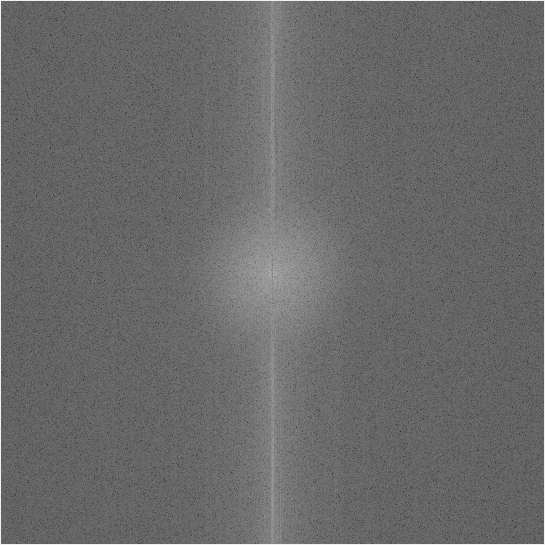
\includegraphics[width=\linewidth]{step1_dp}
		\caption{}
		\label{fig:step1lpf}
	\end{subfigure}%
	\hspace{\fill}
	\begin{subfigure}[b]{0.32\textwidth}
		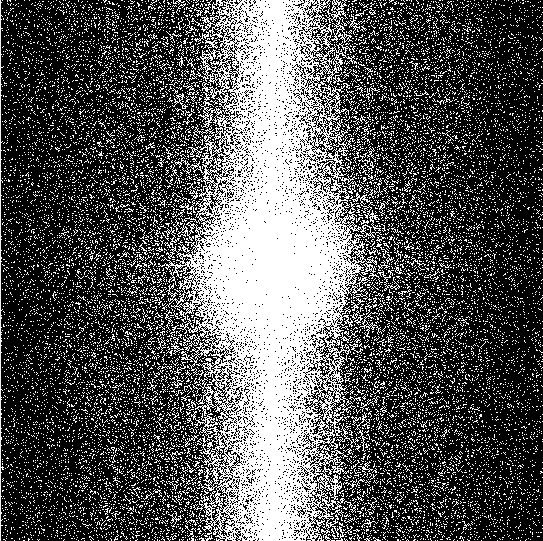
\includegraphics[width=\linewidth]{step2}
		\caption{}
		\label{fig:step2lpf}
	\end{subfigure}%
	\hspace{\fill}
	\begin{subfigure}[b]{0.32\textwidth}
		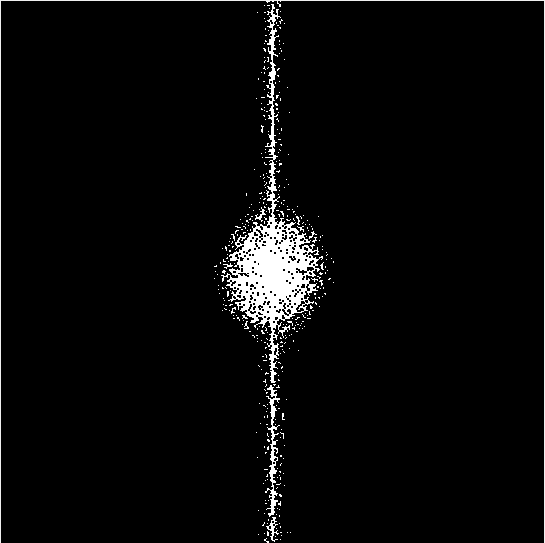
\includegraphics[width=\linewidth]{step3}
		\caption{}
		\label{fig:step3lpf}
	\end{subfigure}%
	\hspace{\fill}
	\begin{subfigure}[b]{0.32\textwidth}
		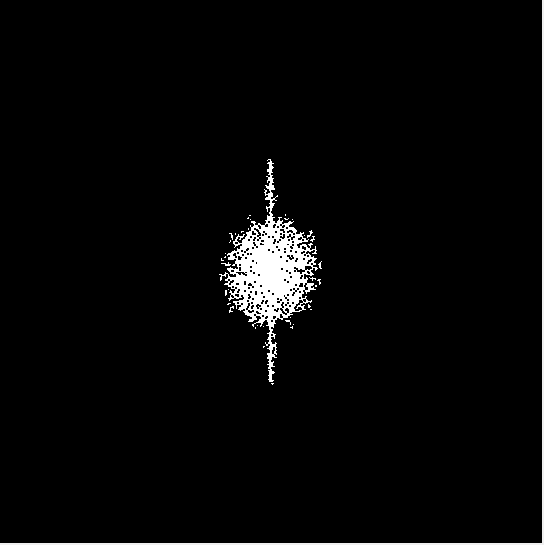
\includegraphics[width=\linewidth]{step4}
		\caption{}
		\label{fig:step4lpf}
	\end{subfigure}%
	\hspace{\fill}
	\begin{subfigure}[b]{0.32\textwidth}
		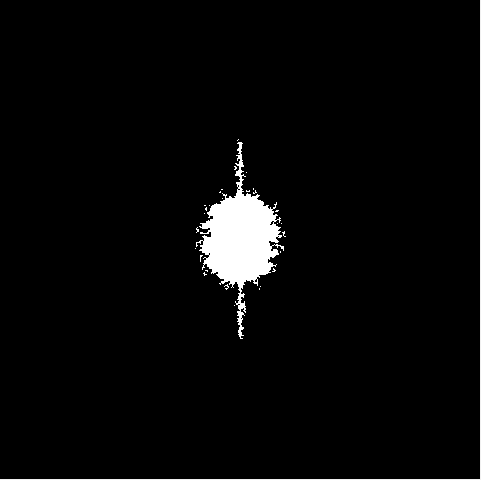
\includegraphics[width=\linewidth]{step5}
		\caption{}
		\label{fig:step5lpf}
	\end{subfigure}%
	\hspace{\fill}
	\begin{subfigure}[b]{0.32\textwidth}
		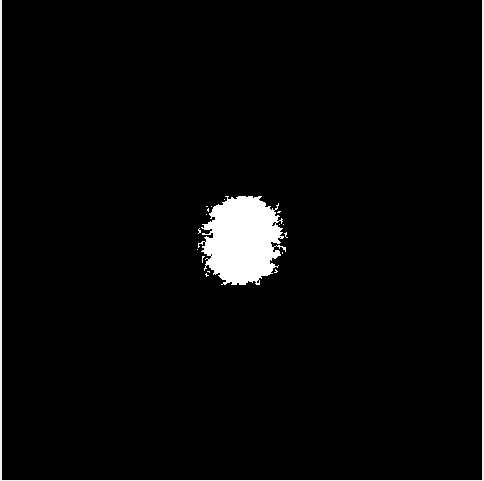
\includegraphics[width=\linewidth]{step6}
		\caption{}
		\label{fig:step6lpf}
	\end{subfigure}%
	\hspace{\fill}
	\begin{subfigure}[b]{0.32\textwidth}
		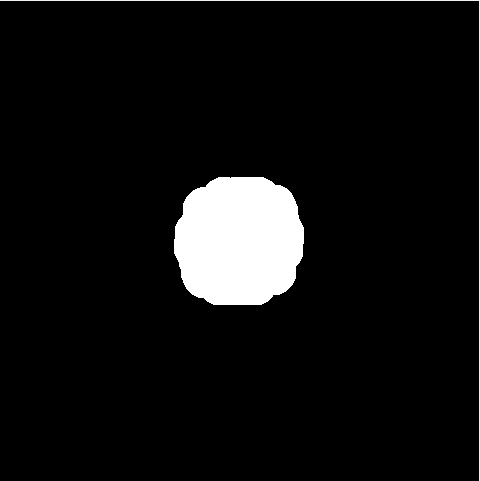
\includegraphics[width=\linewidth]{step7}
		\caption{}
		\label{fig:step7lpf}
	\end{subfigure}%
	\hspace{\fill}
	\begin{subfigure}[b]{0.32\textwidth}
		
\includegraphics[width=\linewidth]{step8}
		\caption{}
		\label{fig:step8lpf}
	\end{subfigure}%
	\hspace{\fill}
	\begin{subfigure}[b]{0.32\textwidth}
		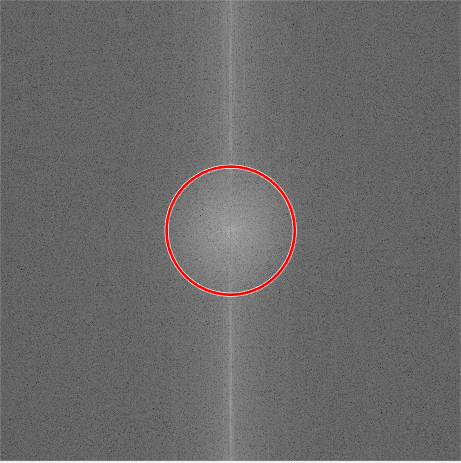
\includegraphics[width=\linewidth]{step9}
		\caption{}
		\label{fig:step9lpf}
	\end{subfigure}
	\caption{Circle detection (a) Amplitude representation of the initial FFT \\transform
		(b) Binary image
		(c) Eroded image (d) largest connected component \\
		(e) After hole filling for (f) Removal of spurious edges
		(g) Dilated image (h) Final result, and (i) comparison between initial and final image}\label{fig:lowpass}
\end{figure}


As input, the method takes an arbitrary gray-value image which then is transformed to the frequency domain with MATLAB fft2 function. For a representation similar to figure \ref{fig:step1lpf} a shifting of the result has to be done as well. 
% add detailed description of FFT functions and usage!
A detailed description of the frequency functions and their specific usage can be found on Mathworks'  \href{http://www.mathworks.com/}{homepage}\footnote{http://www.mathworks.com/}. \\
The complex result has then to be transformed into a gray-value amplitude image in which the imaginary part is discarded and the real part is visualized as a logarithmic absolute value. Now the result is generally the same as above. \\
For the approximation of the circle it is also necessary to convert the image to a binary image. Since only a rough threshold is necessary a simple and fast algorithm for thresholding is used (%needs attention!
built-in Otsu-Thresholding as described in Section \ref{sec:Thresholding}). This rough approximation can be excused due to the clear lack of a distinct circular contour. %still needs attention
This also explains why the implemented circular Hough transform (MATLAB imfindcircles) was not able to deliver satisfying results.\\
\\
In the used dataset sometimes a distinct lack of very low frequencies - equaling a sharp (yet only one pixel in width) line in the center - could be noticed. To rule out similar cases in other datasets as well, a 20x20 pixel white rectangle was inserted in the center (see result section for further discussion).
Afterwards standard erosion with a disk shape is performed. With erosion, noise that persists in the binary image is eliminated by fitting these disks around each black pixel and coloring all pixels within this shape black as well. A detailed explanation on how to define structuring elements such as the used disk and the MATLAB imerode function can be found on \href{http://www.mathworks.com/}{Mathwork}\footnote{http://www.mathworks.com/}. \\
Out of the remaining connected objects the circle now represents the largest one. Hence it is filtered out with MATLAB \begin{verbatim}bwareafilt(.., 1, 'largest') \end{verbatim}
which extracts this largest region and the resulting image has only this central part colored in white. To assure a compact center another operation is performed which fills in enclosed black areas within the circular region 
\begin{verbatim}imfill(...,'holes') \end{verbatim}
The remaining spikes at the top and bottom of the cirlce are removed by deleting every row where there are only a certain number of white pixels. To reverse the erosion process and get a representative circle the MATLAB imdilate operation is performed with a disk structure. \\
MATLAB's regionprops function delivers the centroid as well as the minor and major axis length of the object which then is used to calculate an approximation of the actual radius of the circle. Notice that it is also possible to extract an elliptical structure from non-quadratic images which will not be described in detail here since it does not differ from the steps for a quadratic image. \\
% 03.07 Dennis
For the radius approximation the following formula is used: (insert formula here) \\
Since the removal of the spikes also flattens the circle a bit, it is important to slightly weight the major axis length a bit heavier.  For the distance to the center a 2D-grid is produced by MATLAB ndgrid, using one grid for the distance in x- and one for the distance in y-direction. Afterwards, the distance to the center point is then calculated by the ordinary circular formula to determine whether a point is within the circle (another formula here). Evaluating this formula for each point allows to select the circular region which is then stored as a binary matrix. \\
Finally, the circular region is "cut out" of the original image by multiplying it with the initial fourier transformed image. Before retransforming the image, an inverse shift has to be done with ifftshift. After using ifft2 to recover a spatial form of the image it is also important to transform it back into a uint8 image, using only the real-valued part of the transform. A uint8 image is an image consisting of unsigned 8-bit integer values in the range of 0 to 255.\\
This can all be put together in one code line, resulting in
\begin{verbatim}
image = uint8(real(ifft2(ifftshift(image))));
\end{verbatim}

% changes 03.07 Dennis order swapped with results and comparison
\subsubsection{Advantages over Other Filtering Techniques}
Before comparing the results of the proposed method it should also be discussed why no other filter was used instead.
The biggest issue with filtering techniques is that it is hugely dependent on the available dataset. While others (insert papers with AFM image data here) usually have a pretty distinct noise level and try to optimize for this specific set of images, the goal of this work was to really adapt to various datasets. For different image qualities of AFM pictures, and especially for different resolutions and cutout sizes, results may vary although done by the same instrument or person. \\
Ficarra et al. \cite{ficarra2005automated} use three distinct filtering techniques for the preprocessing step: A 3x3 median filter, an adaptive Wiener filter and a high-pass filter. As for the median filter, the proposed method was also used in this work (compare chapter Median Filter). As a side note it should be mentioned that the median filter has good results for filtering out sudden peaks of noise but is rather inefficient with larger dabs of noise in an image. \\
The mentioned Wiener filter was not pursued any further for the following reasons. First, it works best for a constant noise level which isn't given in all datasets what ultimately let to the design of an own method. Also it is very suitable to clean up the inital data which isn't as much a requirement to this algorithm since it has a fully devoted step of image denoising before filtering out anything. Hence another denoising step would only disturb the image more than it would help remove further artifacts. \\
The problem of the high-pass filter was a bit more subtle. Although it is helpful in providing sharper edges for the later detection of DNA strings, it also attenuates the intensity border between dirt and actual DNA strings (compare section on Histograms). As for the high pass filter itself, it does the exact opposite of a low pass filter: Namely sorting out all of the lower frequency in Fourier space. The aim of Ficarra et al. \cite{ficarra2005automated} was to eliminate noise which was rather low-freuqent but yet again this is a step usually eliminated with denoising in this algorithm. \\
Generally the methods by Ficarra et al. would lead to a much lower rate of actual DNA in the resulting objects and therefore requiring a more subtle decision in whether or not it actually is a DNA string which is currently viewed. By sacrificing a distinct border between the DNA and background, a much lower percentage of noise will be classified as a false positive in the end.

\subsubsection{Results and Comparison}
% 8 images as comparison
% compare the changes in the histogram before and after the filtering steps.
\begin{figure}[H]
	\centering
	\begin{subfigure}[b]{0.321\textwidth}
		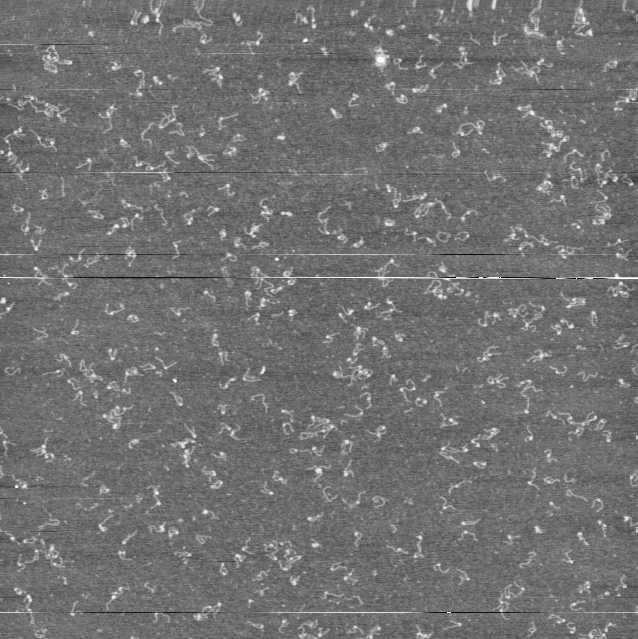
\includegraphics[width=\linewidth]{original}
		\caption{}
		\label{fig:origNoFilt}
	\end{subfigure} 
	\hspace{\fill}
	\begin{subfigure}[b]{0.321\textwidth}
		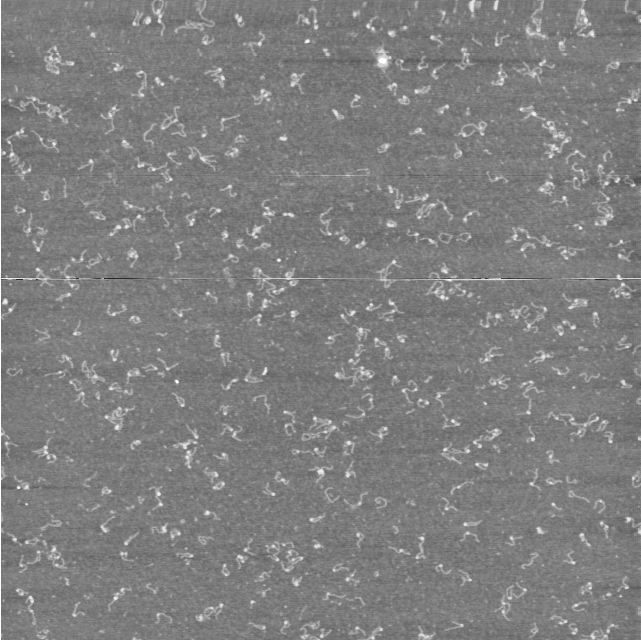
\includegraphics[width=\linewidth]{only_median}
		\caption{}
		\label{fig:onlyMedianFilt}
	\end{subfigure}
	\hspace{\fill}
	\begin{subfigure}[b]{0.321\textwidth}
		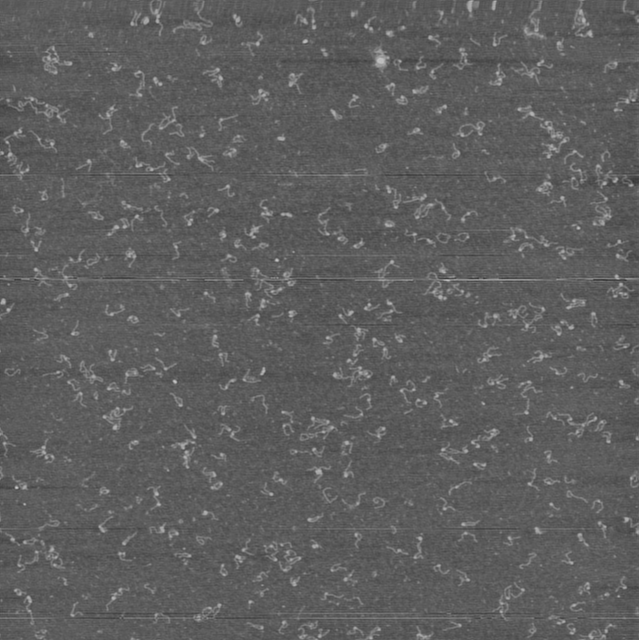
\includegraphics[width=\linewidth]{only_low}
		\caption{}
		\label{fig:soLowFilt}
	\end{subfigure}
	\captionsetup{justification=centering}
	\caption{Comparison between different filtering techniques \\
		(a) original image
		(b) median filter
		(c) low pass filter}
	\label{fig:lowpassCompare1}
\end{figure}

In this part the described low pass filter will be compared to a standard median filter. The used median filter was implemented by Mathworks and the algorithm used is medfilt2 \footnote{http://de.mathworks.com/help/images/ref/medfilt2.html}. In the original image one can see very clearly many noticeable horizontal lines. The occuring of this lines itself makes it obvious again why a good filtering method is needed. And indeed the used median filter removes most of the lines. Only one prominent line in the middle remains. \\
On the third image one can see the effect of the implemented low pass filter. Immediately it is obvious that this image is much darker than the other two images, especially the median filtered. This is due to the fact that the average color of the original image is rather dark. Since the low pass filter averages over the data the result is darker than the original. On AFM images this is nearly always the case. Secondly, in the low pass filterd image one can see more than one horizontal line. Each of these lines is not as prominent as the one extracted by the median filter though.  \\
On the other hand both methods hugely decrease the background noise compared to the original image. However on the low pass filterd image the background is even more uniform.


\begin{figure}[H]
	\centering
	\begin{subfigure}[b]{0.321\textwidth}
		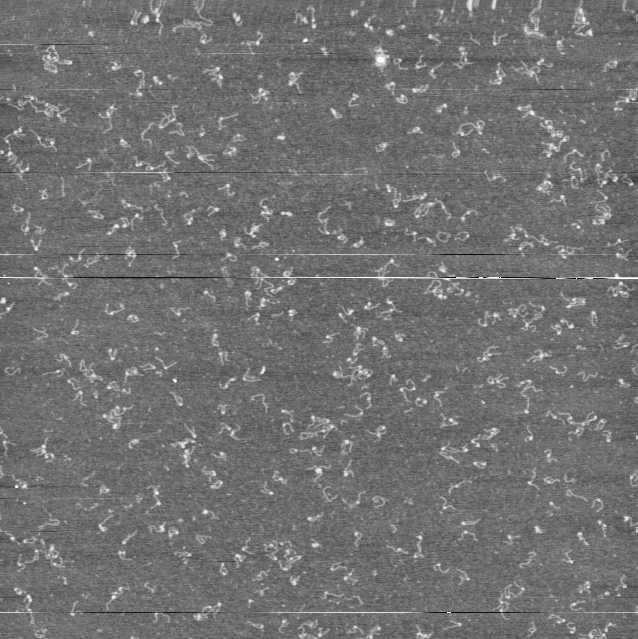
\includegraphics[width=\linewidth]{original}
		\caption{}
		\label{fig:origNoFilt2}
	\end{subfigure} 
	\hspace{\fill}
	\begin{subfigure}[b]{0.321\textwidth}
		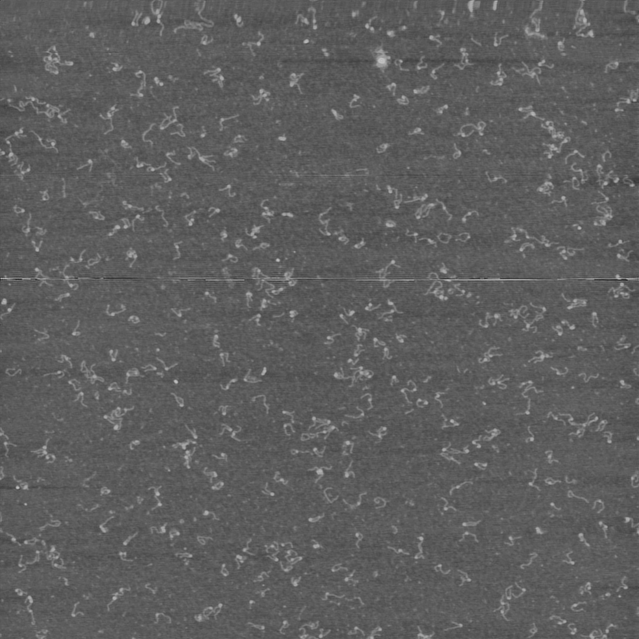
\includegraphics[width=\linewidth]{both_inverse_order}
		\caption{}
		\label{fig:MedianLowPassFilt}
	\end{subfigure}
	\hspace{\fill}
	\begin{subfigure}[b]{0.321\textwidth}
		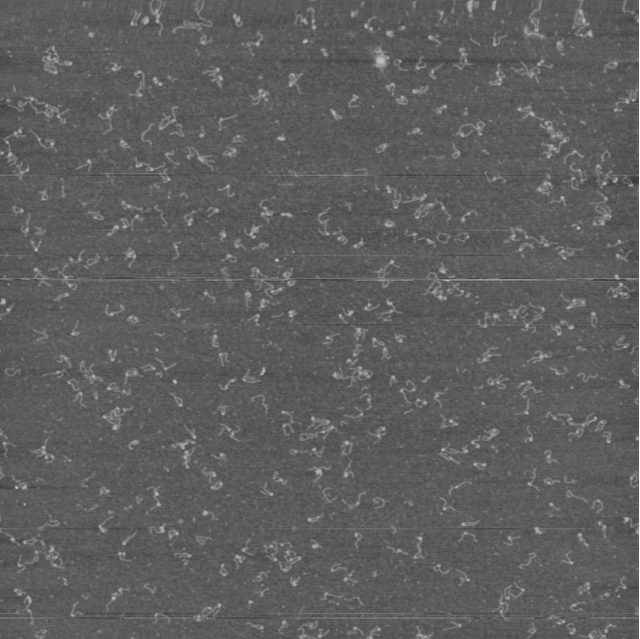
\includegraphics[width=\linewidth]{both_right_order}
		\caption{}
		\label{fig:LowPassMedianFilt}
	\end{subfigure}
	\captionsetup{justification=centering}
	\caption{Comparison between different filtering techniques \\
		(a) original image
		(b) median then low pass filter \\
		(c) low pass then median filter}
	\label{fig:lowpassCompare2}
\end{figure}

Since both filtering methods did not achieve an ideal outcome yet the idea came up to combine both methods. In figure \ref{fig:lowpassCompare2} one can see the original image and a combination of the two filters. On both filtered images a similar effect to above can be observed. If the median filter is applied first the number of horizontal lines are reduced greatly but the remaining line is really prominent. When the low pass filter is used before the median filter the number of lines is higher but the lines itself are smaller and do not stand out as much as in the other case. \\
However, both methods share the advantage that the background is as uniform as the background of an only low pass filtered image. \\
Both of these approaches were implemented and analyzed in regard to their respective results of later processing steps. It could be shown that more useful DNA strands could be extracted by using method \ref{fig:MedianLowPassFilt}. This is in accordance with what one would expect looking at the results above. As a result in this project always the median filter was applied before the low pass filter.\\

\begin{figure}[H]
	\centering
	\begin{subfigure}[b]{0.45\textwidth}
		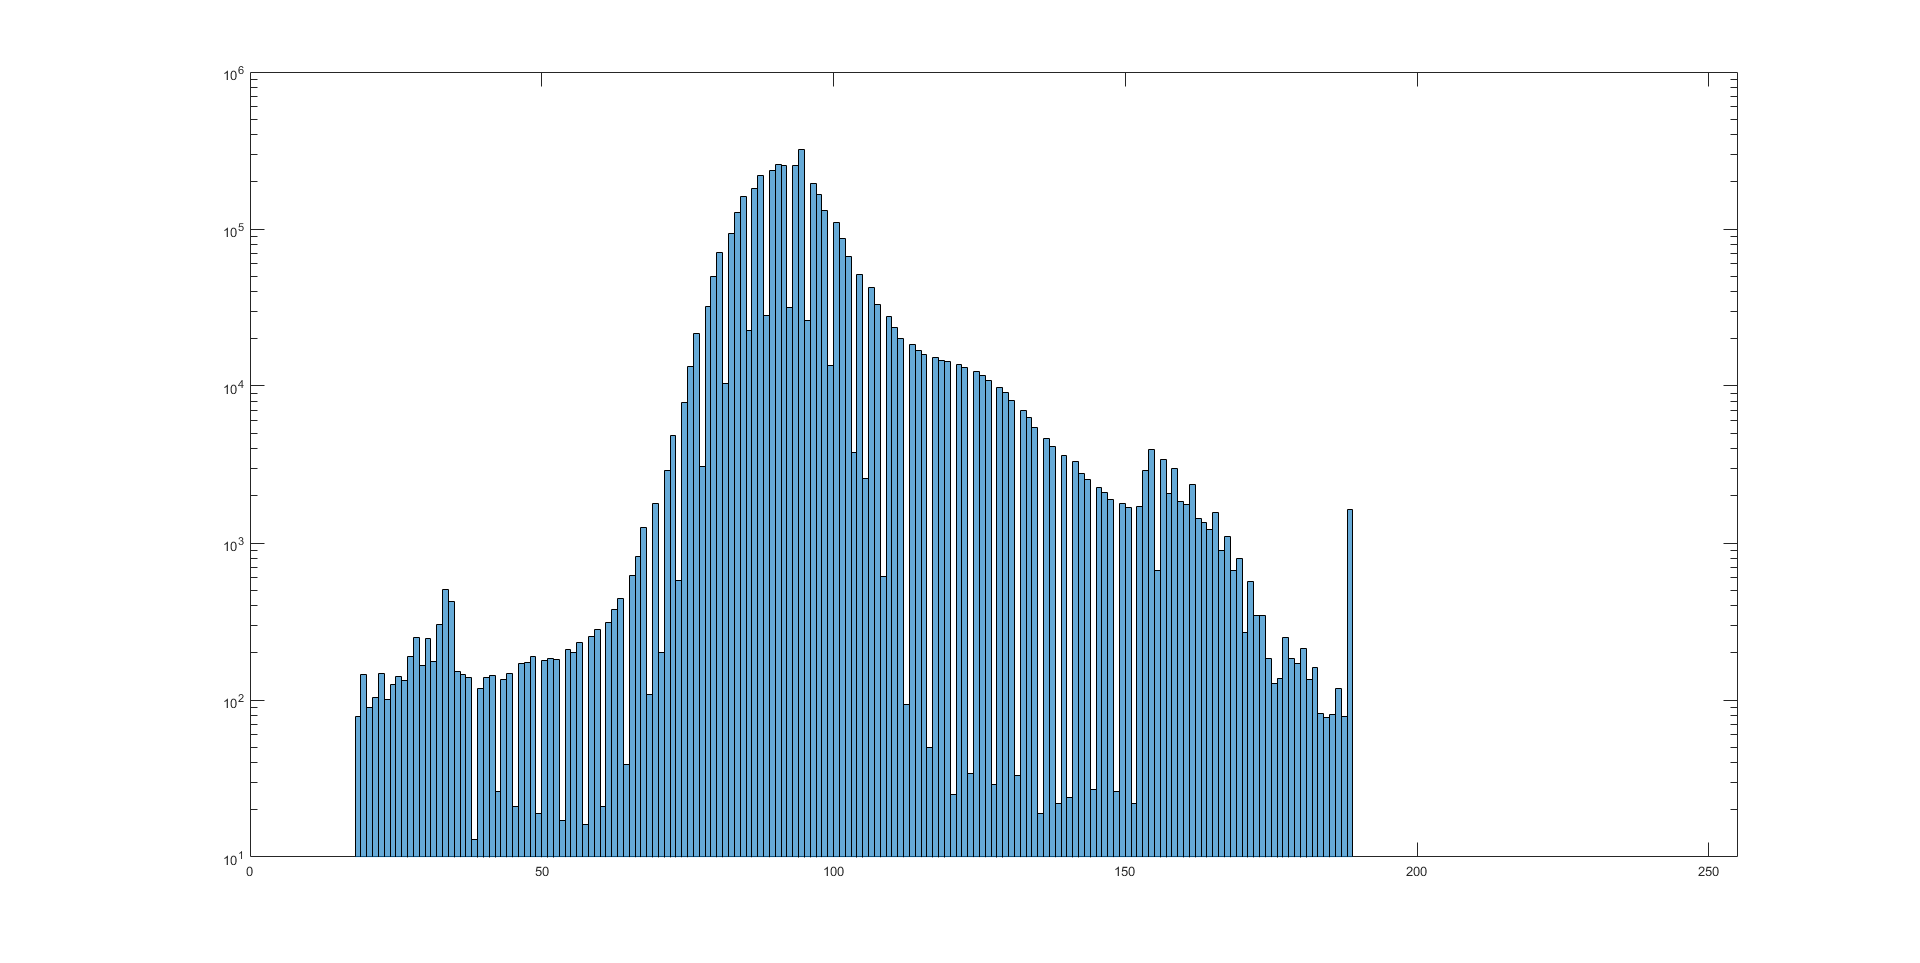
\includegraphics[width=\linewidth]{original_histo}
		\caption{}
		\label{fig:origNoFiltHist}
	\end{subfigure} 
	\\
	\begin{subfigure}[b]{0.45\textwidth}
		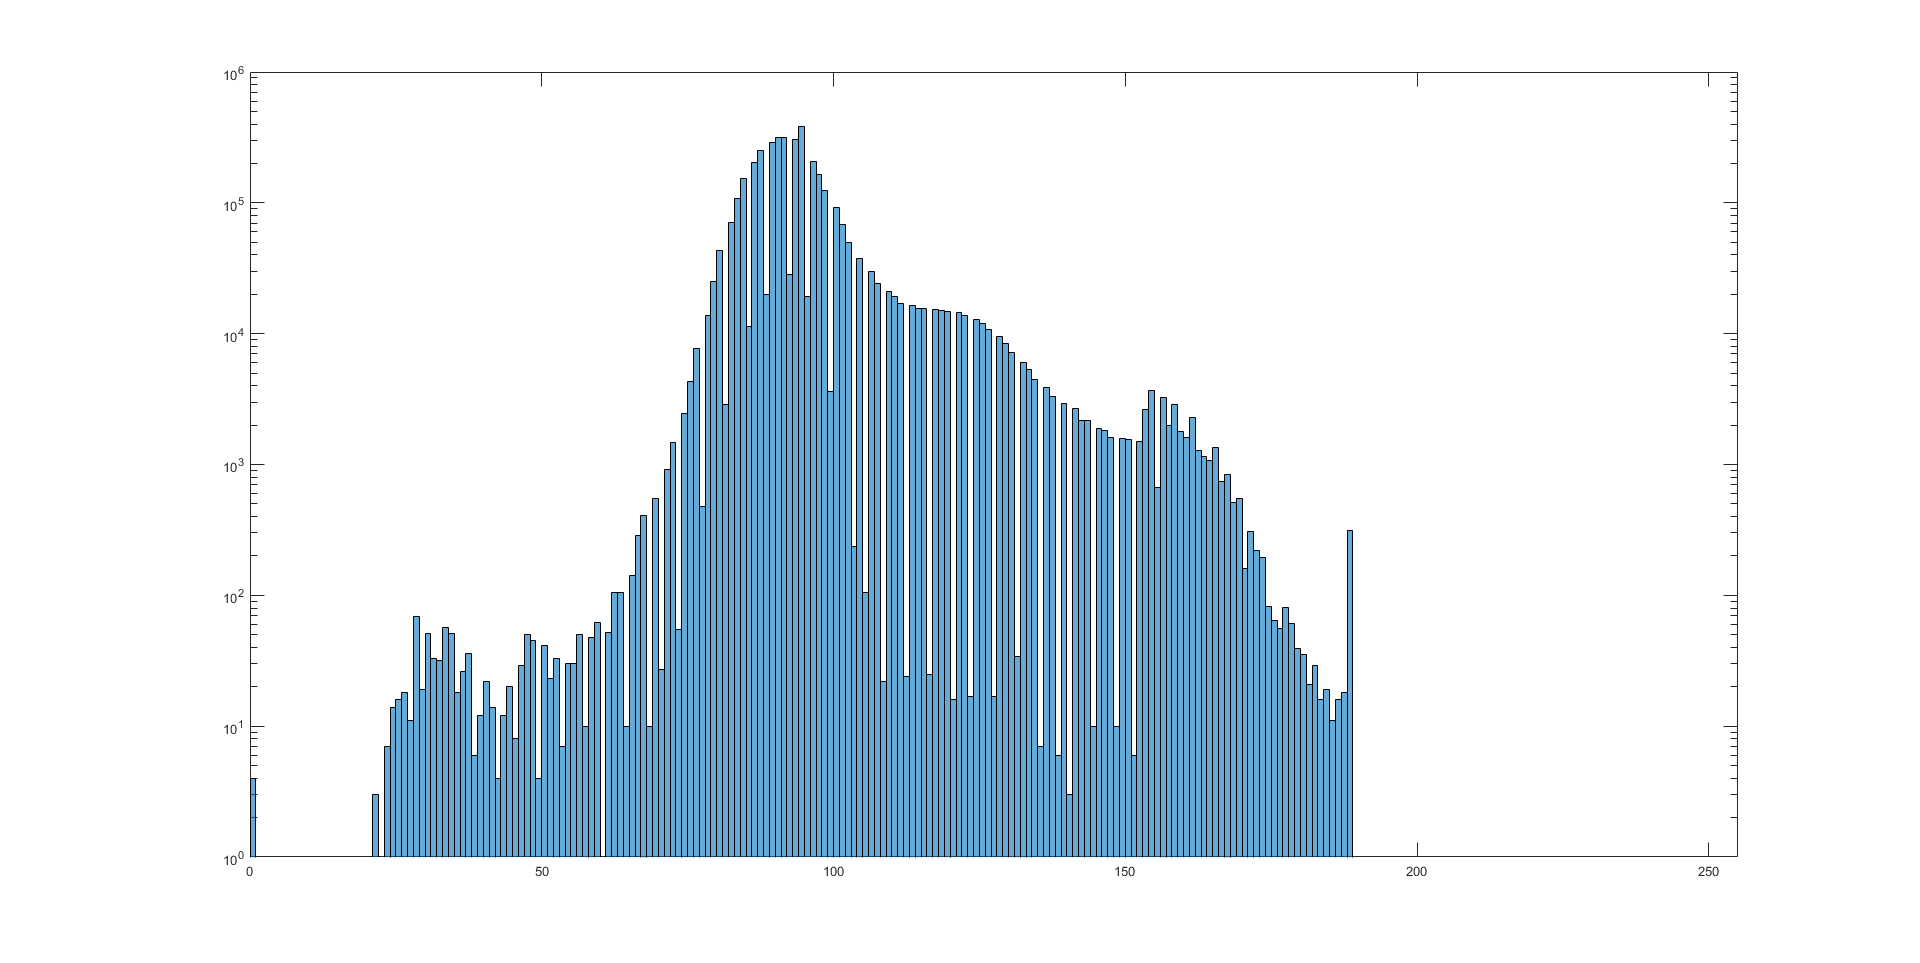
\includegraphics[width=\linewidth]{only_med_histo}
		\caption{}
		\label{fig:MedianFiltHist}
	\end{subfigure}
	\hspace{\fill}
	\begin{subfigure}[b]{0.45\textwidth}
		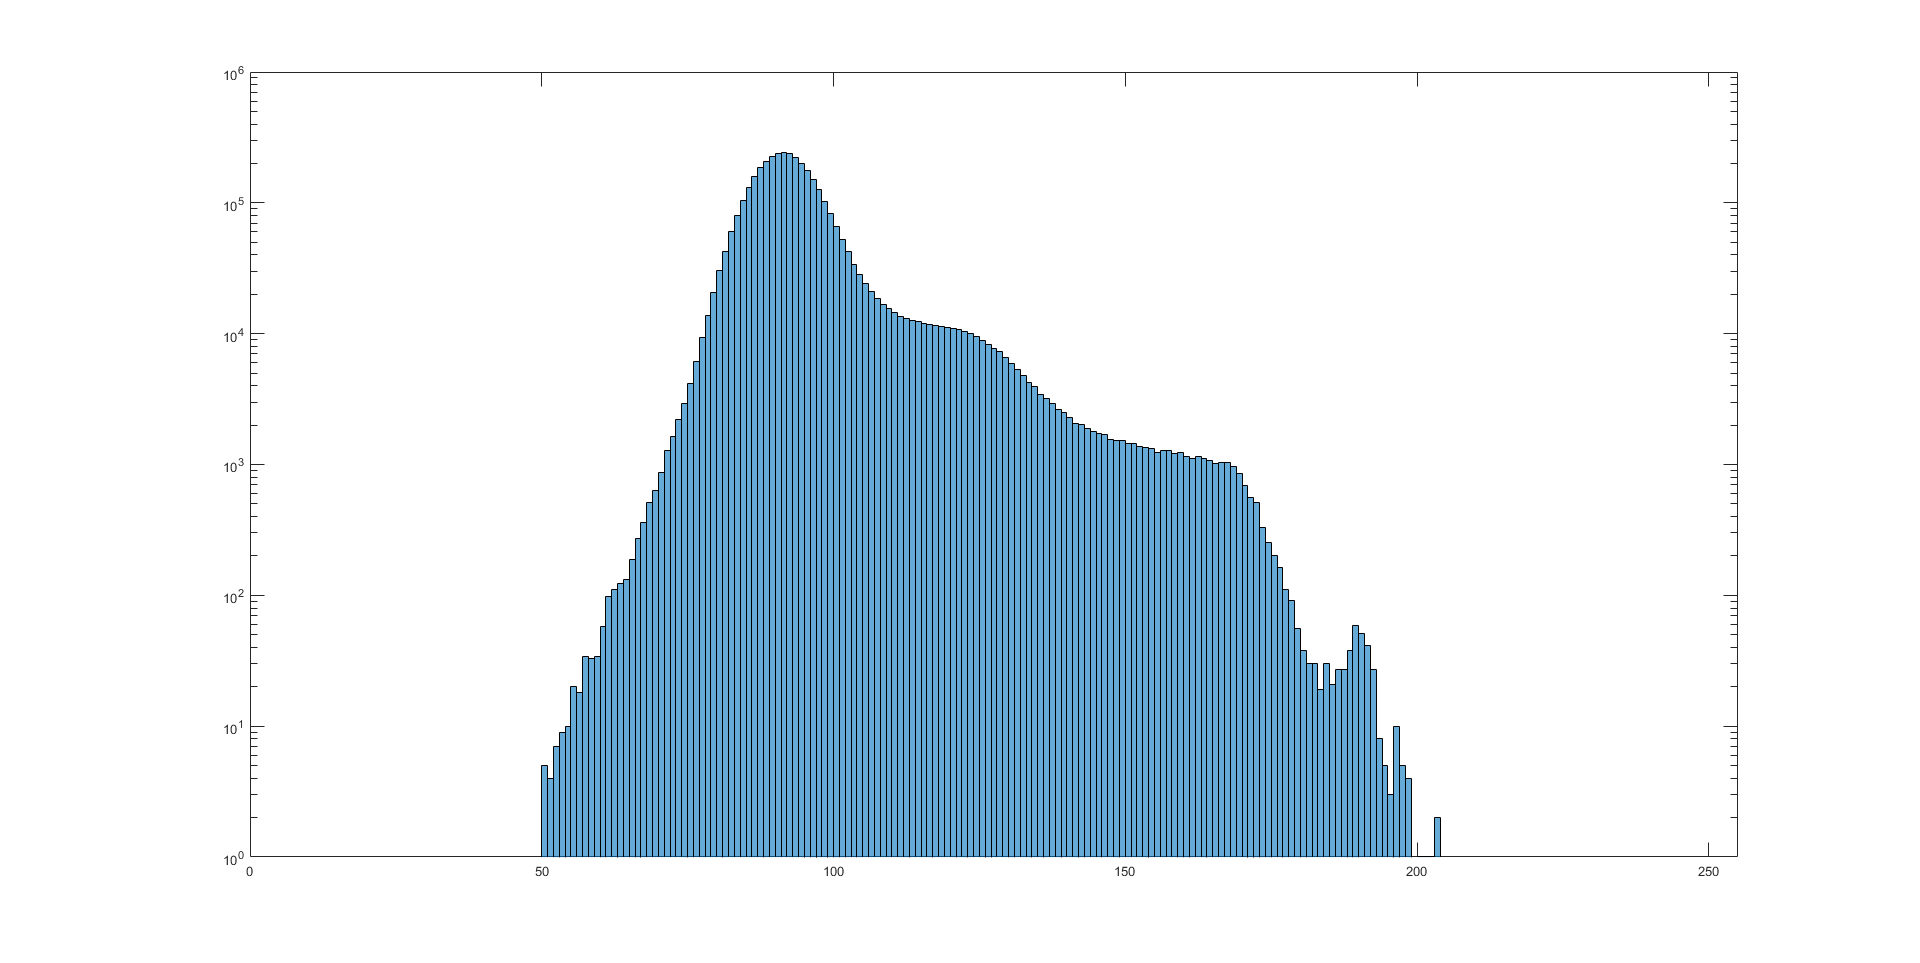
\includegraphics[width=\linewidth]{only_low_histo}
		\caption{}
		\label{fig:LowPassFiltHist}
	\end{subfigure}
	\captionsetup{justification=centering}
	\caption{Histograms of different filtering techniques with logarithmic y-axis scaling. 
		(a) original image
		(b) median filter
		(c) low pass filter}
	\label{fig:lowpassHisto1}
\end{figure}

In figure \ref{fig:lowpassHisto1} three histograms of the original image and after the application of the two filtering techniques can be seen. As one can see in \ref{fig:origNoFiltHist} the original image is lacking an explicit distribution. Many peaks can be observed, especially a striking one at the right end of the spectrum. Obviously there is some shadowing in the distribution as well which makes the distinction between noisy and DNA regions quite hard because a patch consisting of only a few pixels of the same value might still be in range of the values the DNA consists of.\\
In comparison the median filtered image does look very similar at first glance. However, a better distinction can be observed at lower values while at higher values the distribution does not differ as much and there is a very striking peak at 0 which is irritating but negligible. A big advantage can be seen regarding the shadowing of the values. The shadowed peak is much narrower than in the non-filtered image and the low points in medium range are not as low as before. On the other hand the slope of the peak is much higher which is useful for differentiating between background and DNA objects. \\
The histogram of the low pass filtered image \ref{fig:LowPassFiltHist} is eliminating the shadowing problem. The distribution of the values is really smooth after this processing step. One can observe that low values below 50 are cancelled out which leads to the impression that the slope is steeper than before. In truth only the distribution of the values has changed. On the other side of the spectrum the high peak is smoothed out too which leads to higher values than in the original image. This shift to higher values leads to the herein before mentioned effect of darkening the picture. On the other hand the general distribution of the values remains the same and the peak is not narrowed as it is by using the median filter. Similar results can be observed in all images.


\begin{figure}[H]
	\centering
	\begin{subfigure}[b]{0.45\textwidth}
		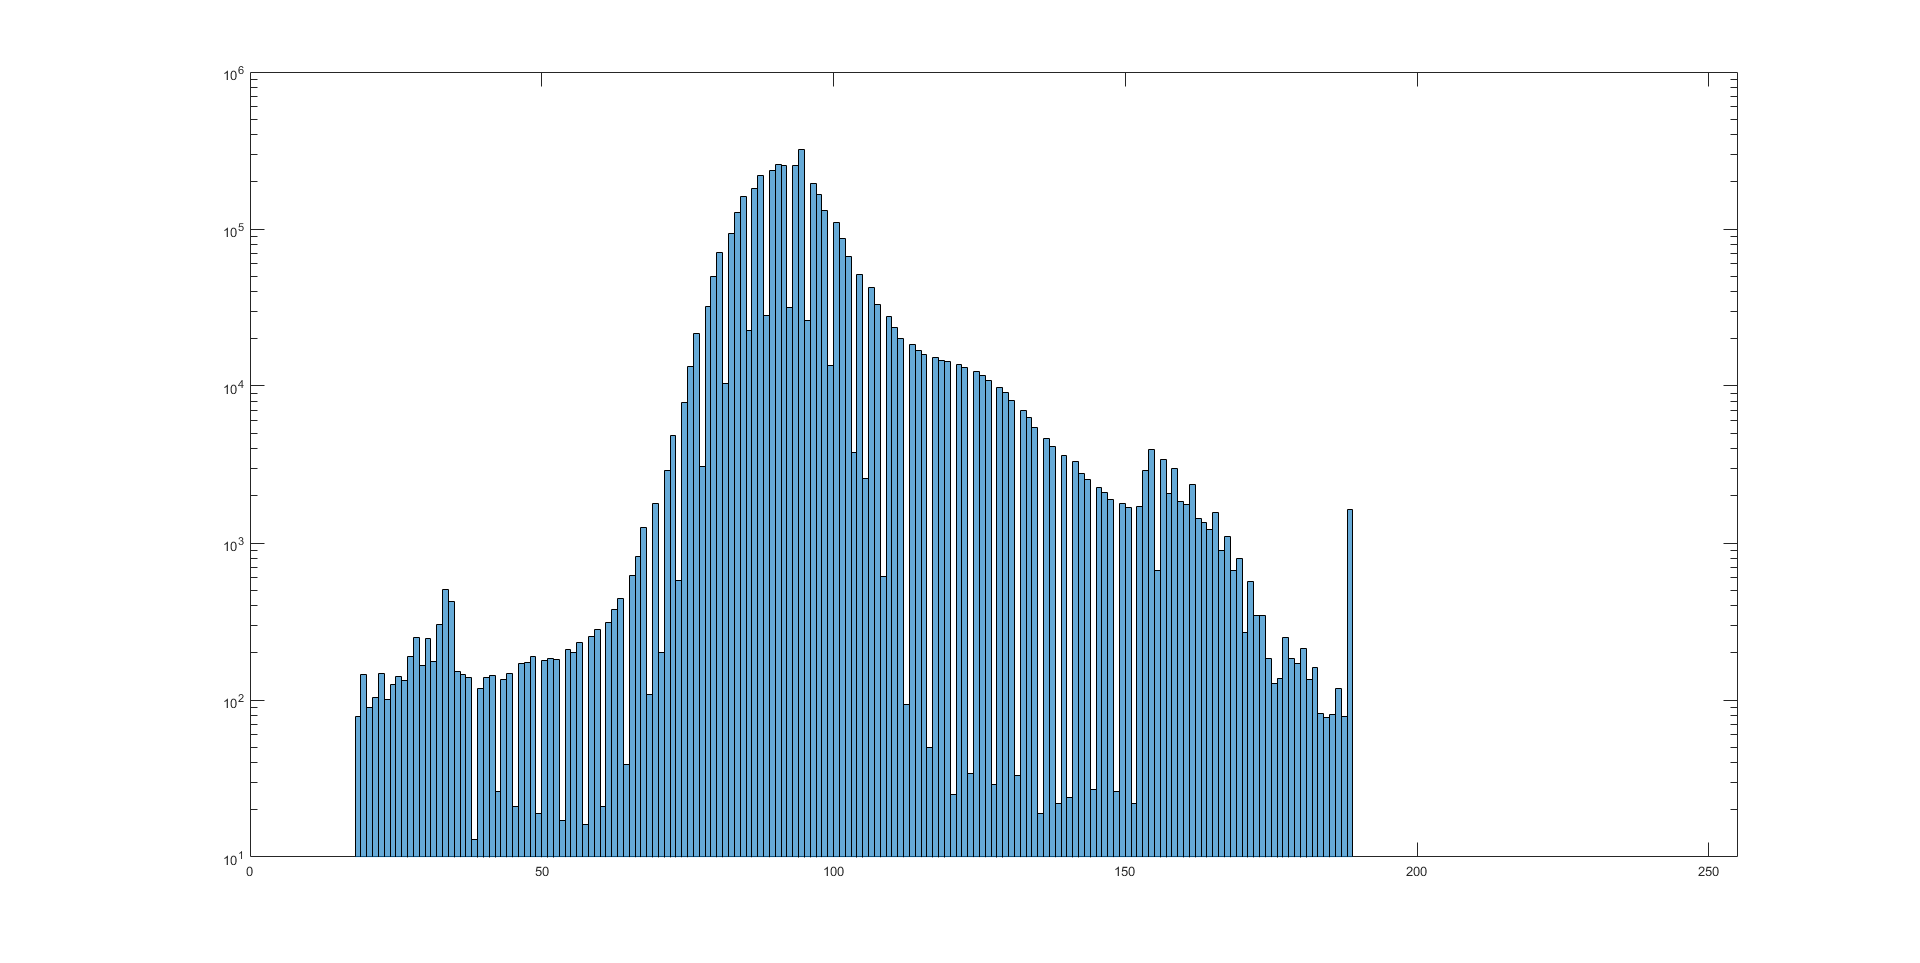
\includegraphics[width=\linewidth]{original_histo}
		\caption{}
		\label{fig:origNoFiltHist2}
	\end{subfigure} 
	\\
	\begin{subfigure}[b]{0.45\textwidth}
		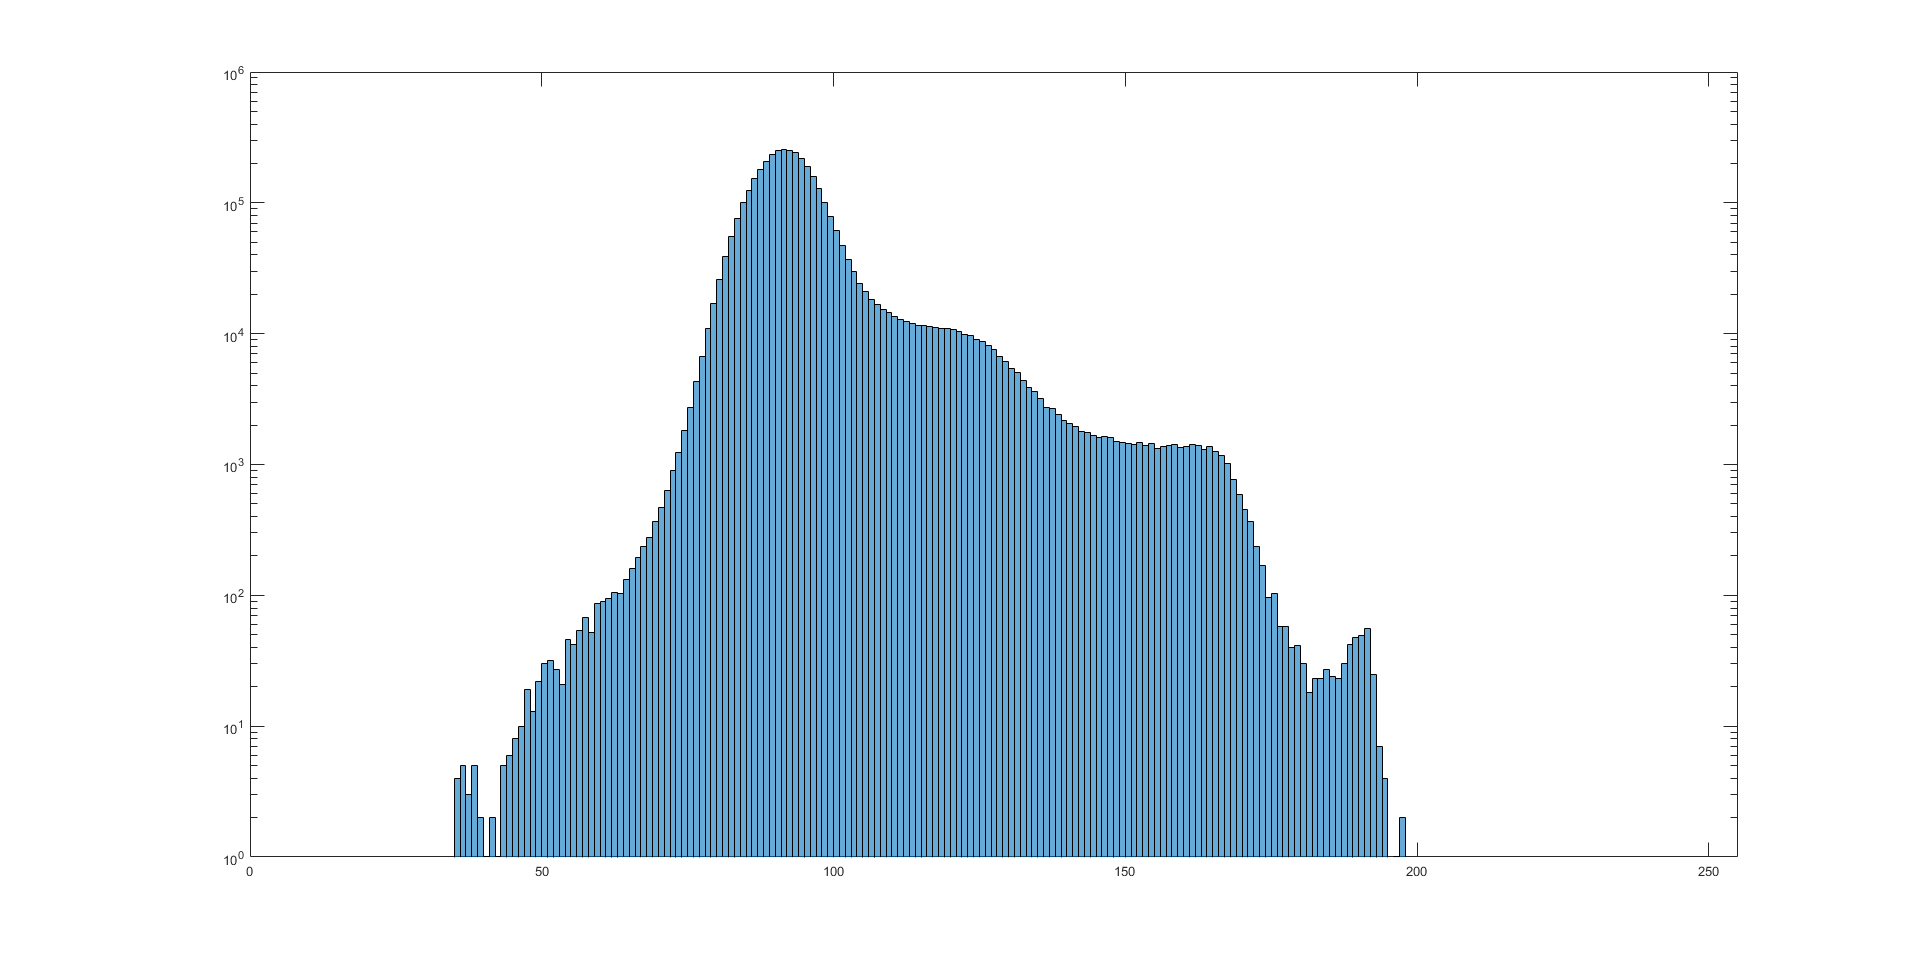
\includegraphics[width=\linewidth]{both_inverse_histo}
		\caption{}
		\label{fig:MedianLowPassFiltHist}
	\end{subfigure}
	\hspace{\fill}
	\begin{subfigure}[b]{0.45\textwidth}
		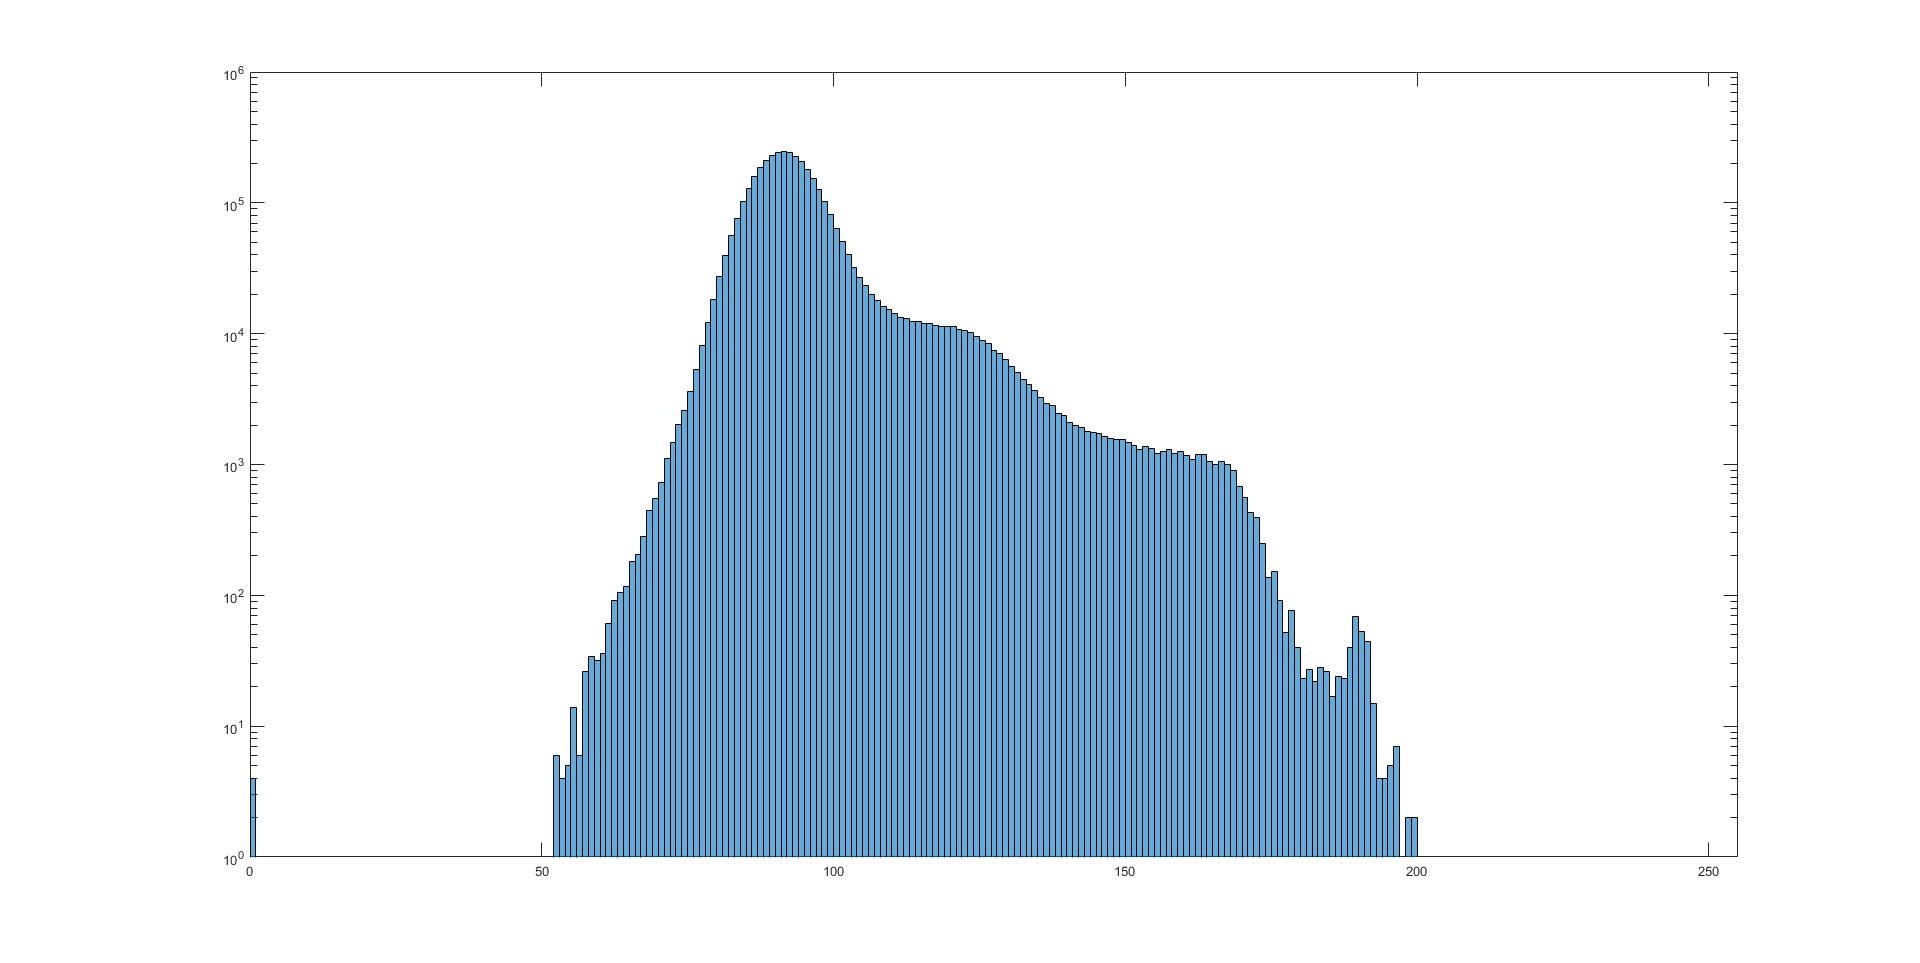
\includegraphics[width=\linewidth]{both_right_histo}
		\caption{}
		\label{fig:LowPassMedianFiltHist}
	\end{subfigure}
	\captionsetup{justification=centering}
	\caption{Histograms of different filtering techniques with logarithmic y-axis scaling.
		(a) original image
		(b) median then low pass filter \\
		(c) low pass then median filter}
	\label{fig:lowpassHisto2}
\end{figure}

In figure \ref{fig:lowpassHisto2} the result of the combination of the two filtering techniques can be observed. Both sequences share the trait of the low pass filter that there is no shadow anymore and that the values are higher overall. The high peak at the end of the spectrum has vanished in both cases too. \\
When the low pass filter is applied before the median filter one can see a peak at 0 again. If the algorithms are executed in the reverse order this effect vanishes and pixel values below 50 exist which does not matter much but should be considered nonetheless. In case \ref{fig:MedianLowPassFiltHist} the slope between values of 50 and about 90 is a bit steeper than in case \ref{fig:LowPassMedianFiltHist} and the values are more equally distributed at pixel values betwenn 130 and 170. \\
The steeper slope explains the results that could be observed earlier. By applying the median filter first the DNA and the background can be distinguished better. Another useful property is that the upper bounds are clearly discernible through a steep slope as well. Although this wasn't particularly helpful in the used dataset, it might come in handy for normalized datasets. The reason behind that is that a normalized dataset (with uniform gray-values for DNA strands) would allow to reject noise peaks as well. As mentioned before, in the used dataset no such normalization was performed which led to further spread values for DNA and would not allow a discernible region for noise.
\\ One should keep in mind that the peak is not the DNA but the background. So a clear peak at values of around 100 extracts the background perfectly. The results seen in \ref{fig:MedianLowPassFiltHist} confirm the impression given earlier in figure \ref{fig:lowpassCompare2} that applying the median filter and then the low pass filter deliver the best results.

\subsection{Thresholding}\label{sec:Thresholding}
After denoising and the subsequent application of our filter combination, the next logical step is to determine a threshold for the binarization of each image. Binarization means that each pixel of an image can be classified either as background or as belonging to a potential DNA strand / nucleosome. It is done by computing a specific gray value, the threshold, each pixel's gray value is compared to in order to classify it.\\
In a first approach, we tried several different thresholding algorithms, such as Intermeans-, Moments-, Intermodes-, Maxentropy-, Minerror-, Percentile- and Otsu-Thresholding. Except for the last, all of these were adapted from GNU Octave (\cite{GNUOctave}), since MATLAB only provides the Otsu-Thresholding method. GNU Octave is an open source high-level numerical computation language comparable to MATLAB. Some of them determine a global threshold, some a local. However, after several tests especially in conjunction with the rest of our Thresholding algorithm we found that Otsu-Thresholding provided us with the best results (data not shown).\\
The greatest problem was that many images still contained noise types that have not yet been removed but that had a strong influence during the computation of these thresholds. If not removed, the corresponding threshold will be so much distorted that meaningful / useful binarization will not be possible.\\
Therefore, an adaptive thresholding algorithm (see \ref{sec: Adaptive Thresholding}) was designed that allowed us, on any image, to create a much more uniform background. This step is one of the main reasons for the general robustness of our routine towards different noise sources.

\subsubsection{Adaptive Thresholding}\label{sec: Adaptive Thresholding}
The TIFF images often vary in intensity, distribution and scaling of the height profile of the DNA samples. This presents a couple of problems for the thresholding algorithms, such as pollution of some image regions which distort the threshold. As discussed above, these issues lead to a false classification of the DNA strands or even to a complete loss of image information.
Two sorts of noise persist after the initial pipelining steps  
Opencv Denoising, LowPassFilter and Median Filter (see Sections \ref{sec:Denoising}, \ref{sec:Filtering}).
\begin{figure}[!htb]
	\begin{subfigure}{0.5\textwidth}
		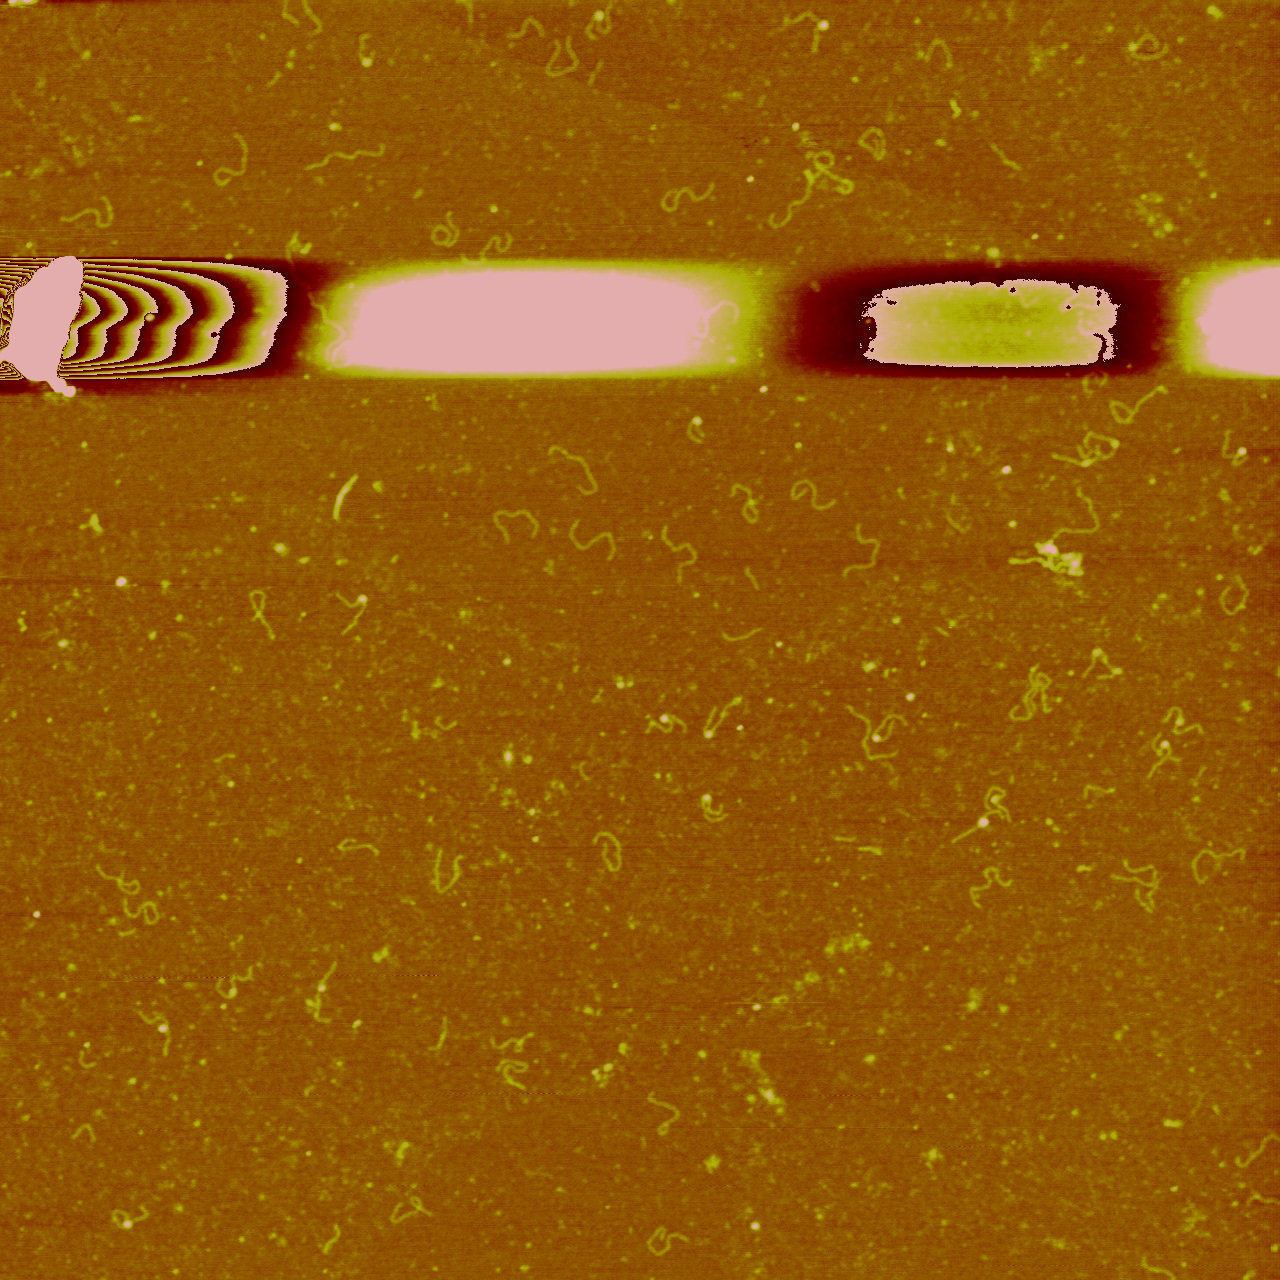
\includegraphics[width=\linewidth]{noise1.png}
		\caption{}
		\label{fig: Noise1}
	\end{subfigure}%
	\hspace{\fill}
	\begin{subfigure}{0.5\textwidth}
		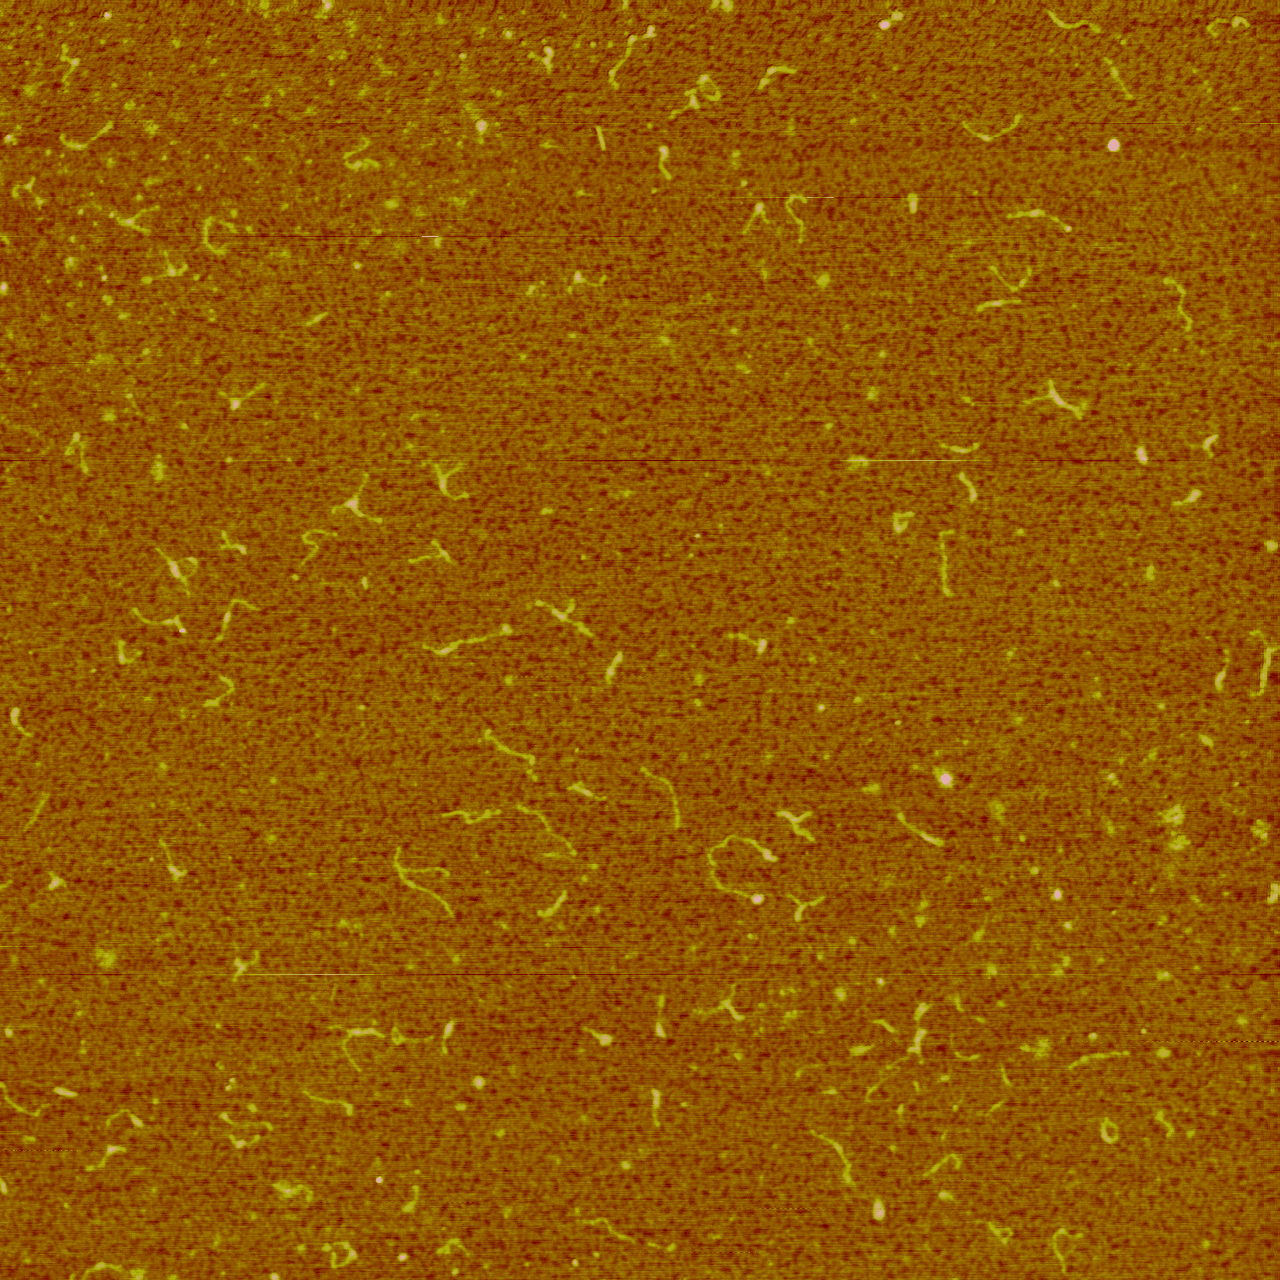
\includegraphics[width=\linewidth]{noise2.png}
		\caption{}
		\label{fig: Noise2}
	\end{subfigure}%
	\caption{(a)Noise Example 1 (b)Noise Example 2}\label{fig:Noise1Noise2}
\end{figure}
\\
The first type of noise as seen in Figure \ref{fig: Noise1} are large distorted regions in the upper value range at an approximate height of 190. If not handled these regions lift the threshold to a level where DNA-strands are missed entirely. 
The second sort of noise seen in Figure \ref{fig: Noise2} consists of small imperfections scattered over the whole image.
Unfortunately the height profile of these imperfections is very similar to the one of the DNA-strands and it is therefore very hard to automatically distinguish between them.
The overwhelming majority of disturbance on the images observed is part of the first type.
The aim of this part of the pipeline is to pre-process the data by three additional steps which treat the outliers in the upper value range and if possible improve detection and removal of scattered noise.

In order to tackle these issues the following three step method is proposed:
\begin{enumerate}
	\item Homogenize the background to provide a consistent and distinguishable layer on which the DNA-strands can be recognized easily.
	\item Identify and remove polluted image regions and outliers in the upper intensity values.
	\item Limit the threshold to an appropriate range.
\end{enumerate}
\subsubsection{Level Background}\label{sec: Level Background}

Figure \ref{fig:HistThresh} shows a histogram of the height values of a representative original image from the dataset.
In the observed dataset DNA-strands can only be found in an intensity range from about 110 to 160, while nuclei can be found between 160 and 200.


\begin{figure}[!htb]
	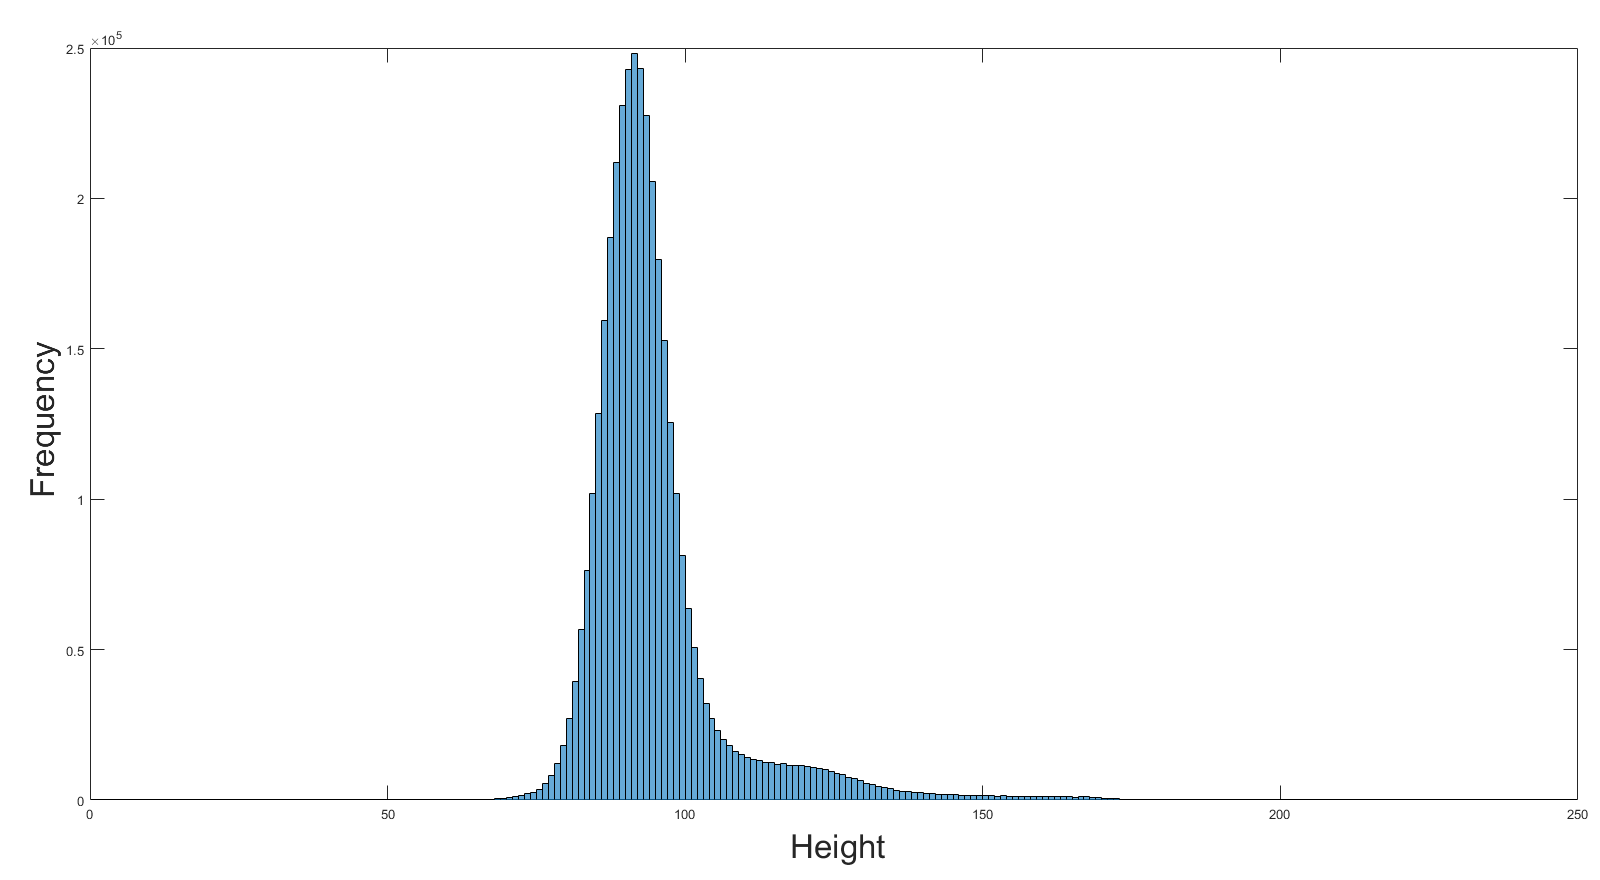
\includegraphics[width=1\linewidth]{histogramOriginal.png}
	\caption{Histogram of TIFF image}
	\label{fig:HistThresh}
\end{figure}
The accumulation point at a value of 95 is distinctive for background noise. 
Therefore, smaller values are set to this boundary.
This approach creates a more consistent background for all images and limits the variation due to noise.
It is important to mention that this method can only be used after the lowPassFilter which smooths the height distribution and thereby guarantees that only noise is removed. If applied to the raw unfiltered image this method will also remove outliers within the DNA-strands which results in perforated DNA objects.
The resulting image shown in Figure \ref{fig:background} yields a more consistent threshold and with that a higher error resistance.


\begin{figure}[!htbp]
	\begin{subfigure}{0.5\textwidth}
		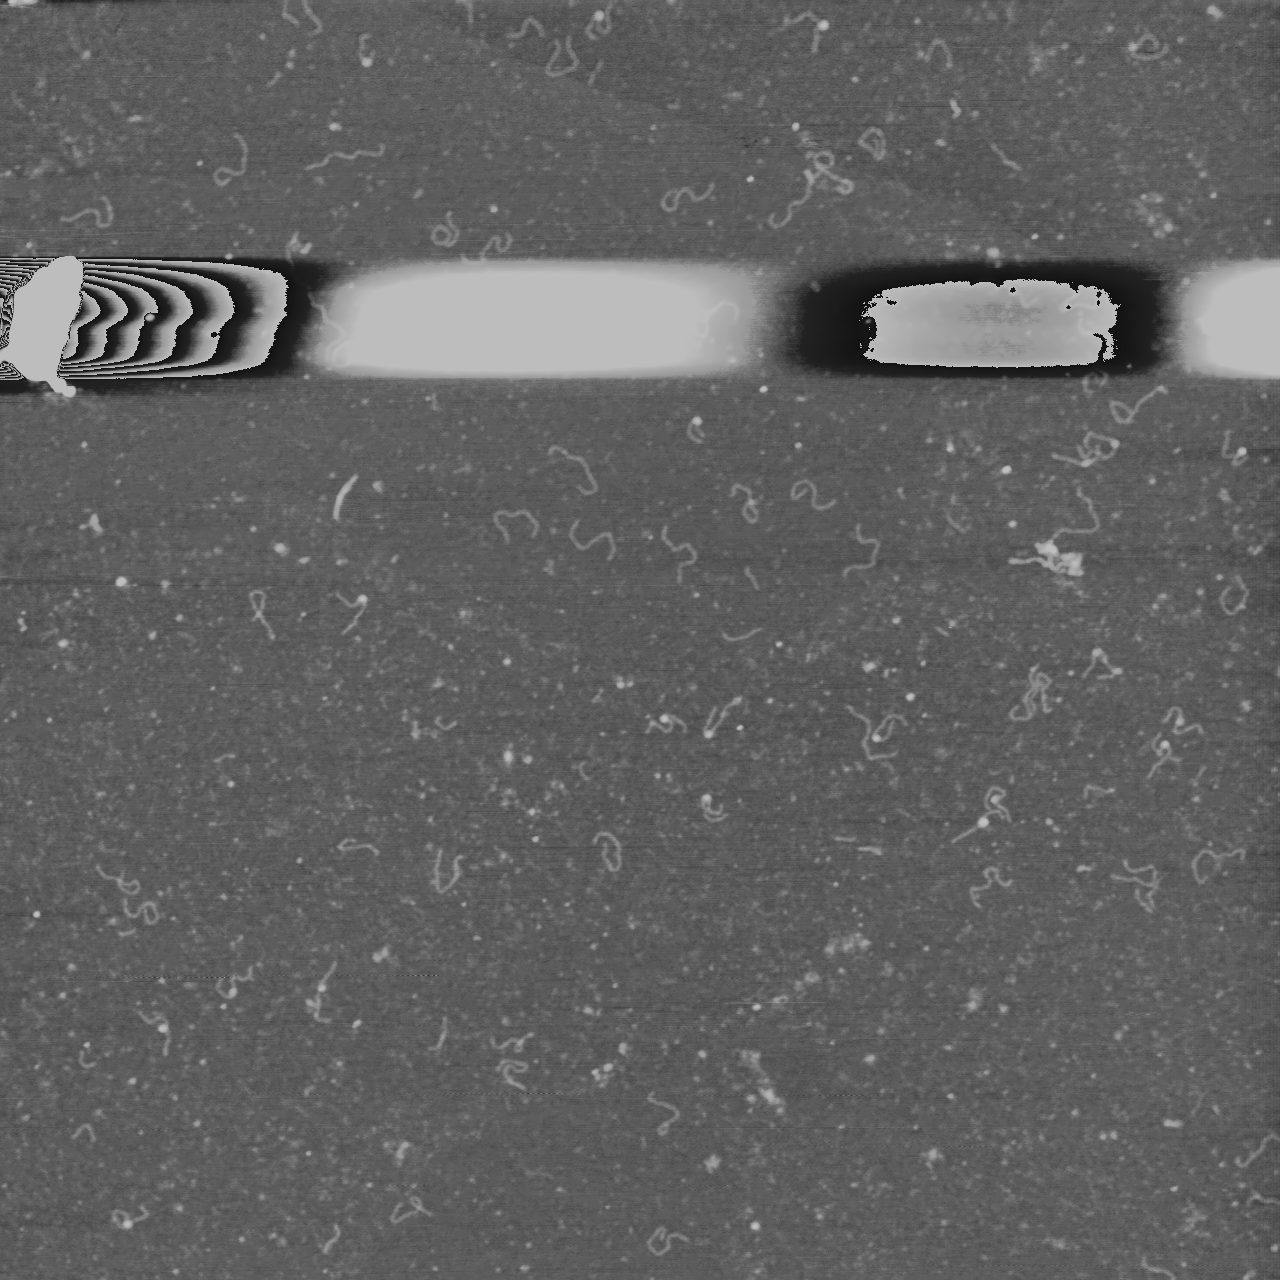
\includegraphics[width=\linewidth]{noise21.png}
		\caption{}
		\label{fig:rawImage}
	\end{subfigure}%
	\hspace{\fill}
	\begin{subfigure}{0.5\textwidth}
		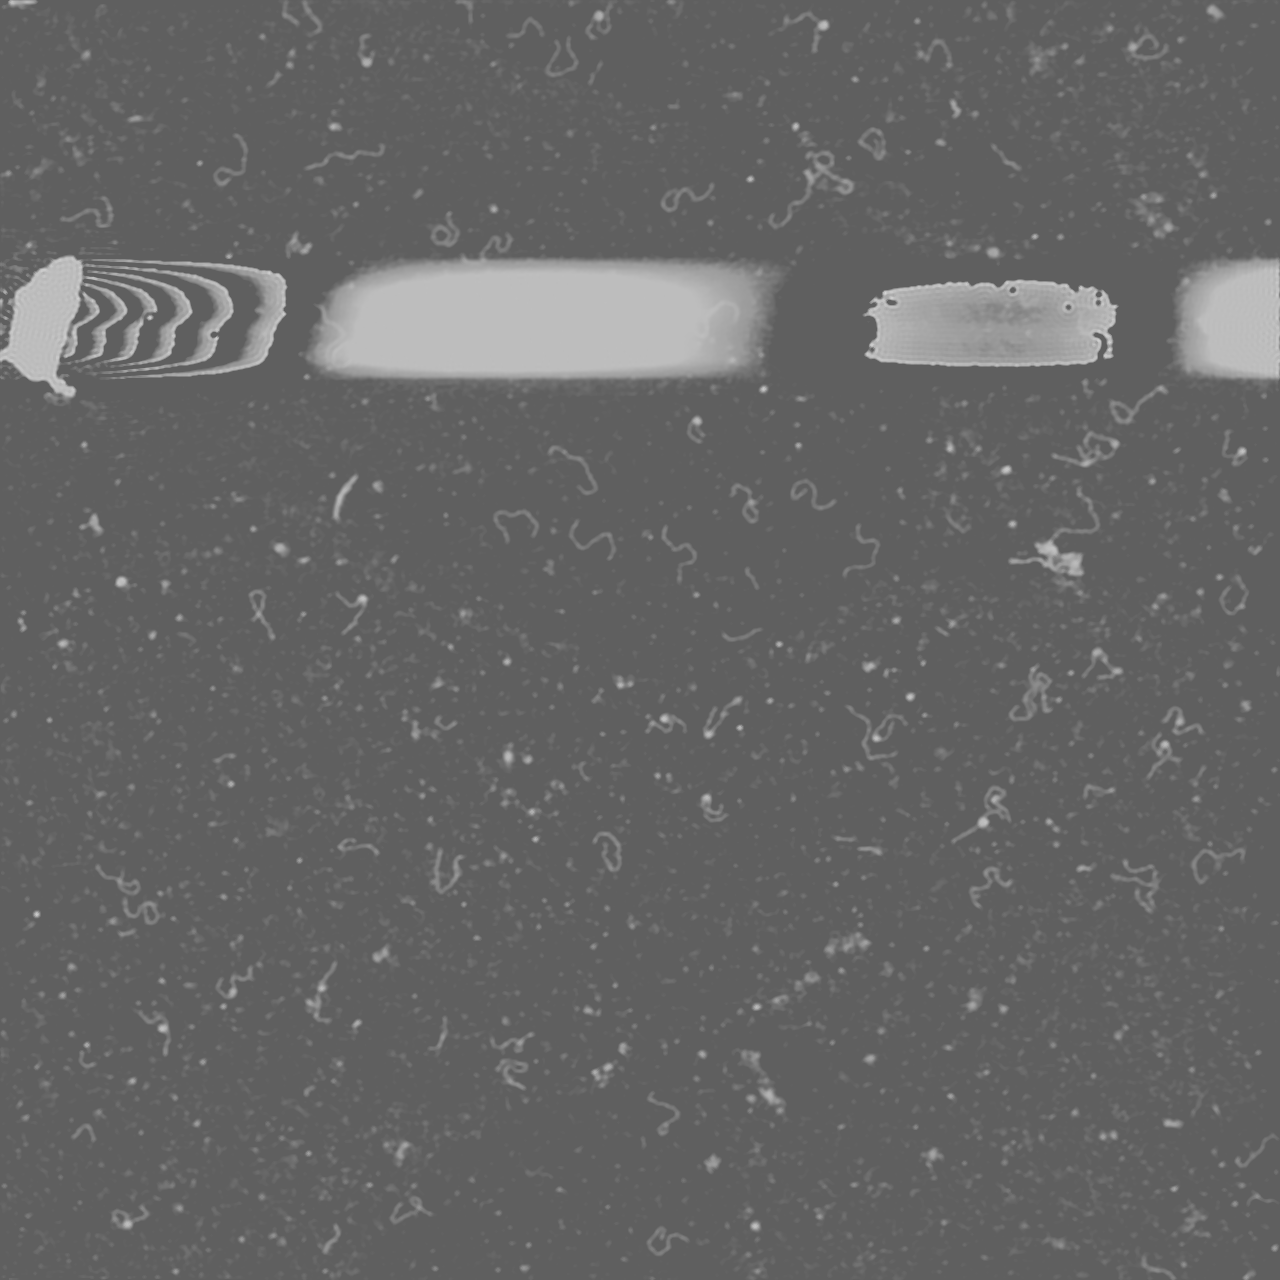
\includegraphics[width=\linewidth]{step21.png}
		\caption{}
		\label{fig:step1}
	\end{subfigure}%
	\caption{(a)Before leveling (b)After leveling }\label{fig:background}
\end{figure}
\subsubsection{Identify and remove outliers} \label{sec: Outlier Removal}
At first a global threshold algorithm like the Otsu method (see section \ref{sec:Thresholding}) is used to create a binary image.
All objects that could be a DNA object are removed based on size. Now only noise and other non-DNA objects are left.

\begin{figure}[!htb]
	\begin{subfigure}{0.5\textwidth}
		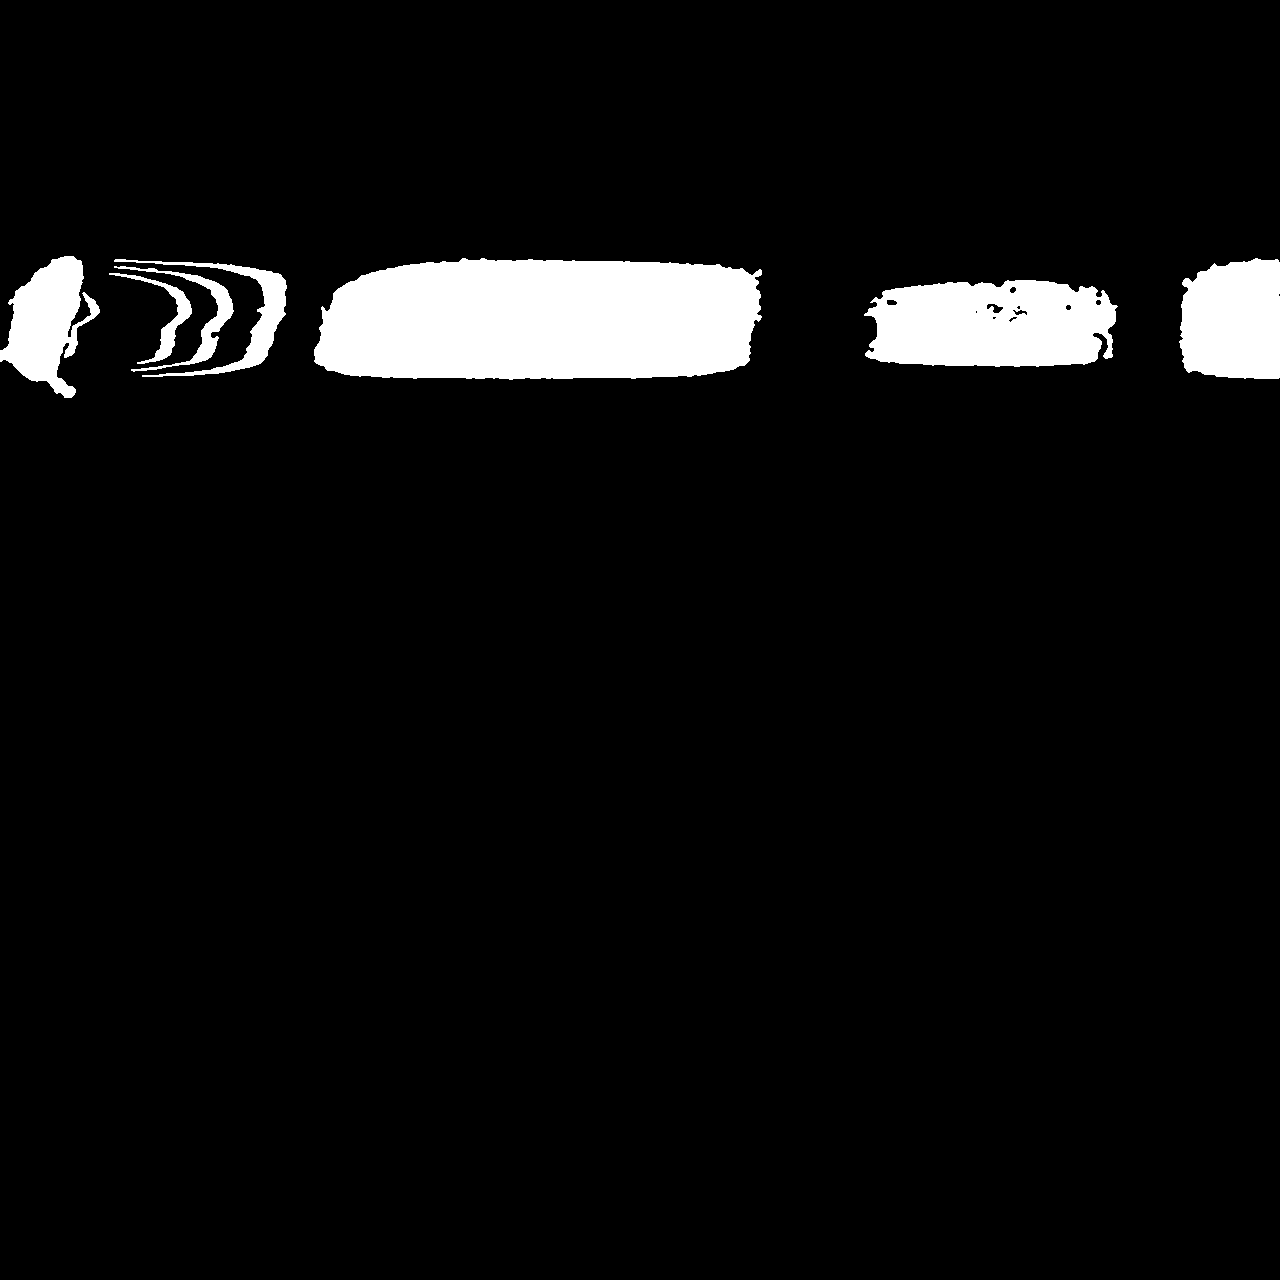
\includegraphics[width=\linewidth]{Maske.png}
		\caption{}
		\label{fig:mask}
	\end{subfigure}%
	\hspace{\fill}
	\begin{subfigure}{0.5\textwidth}
		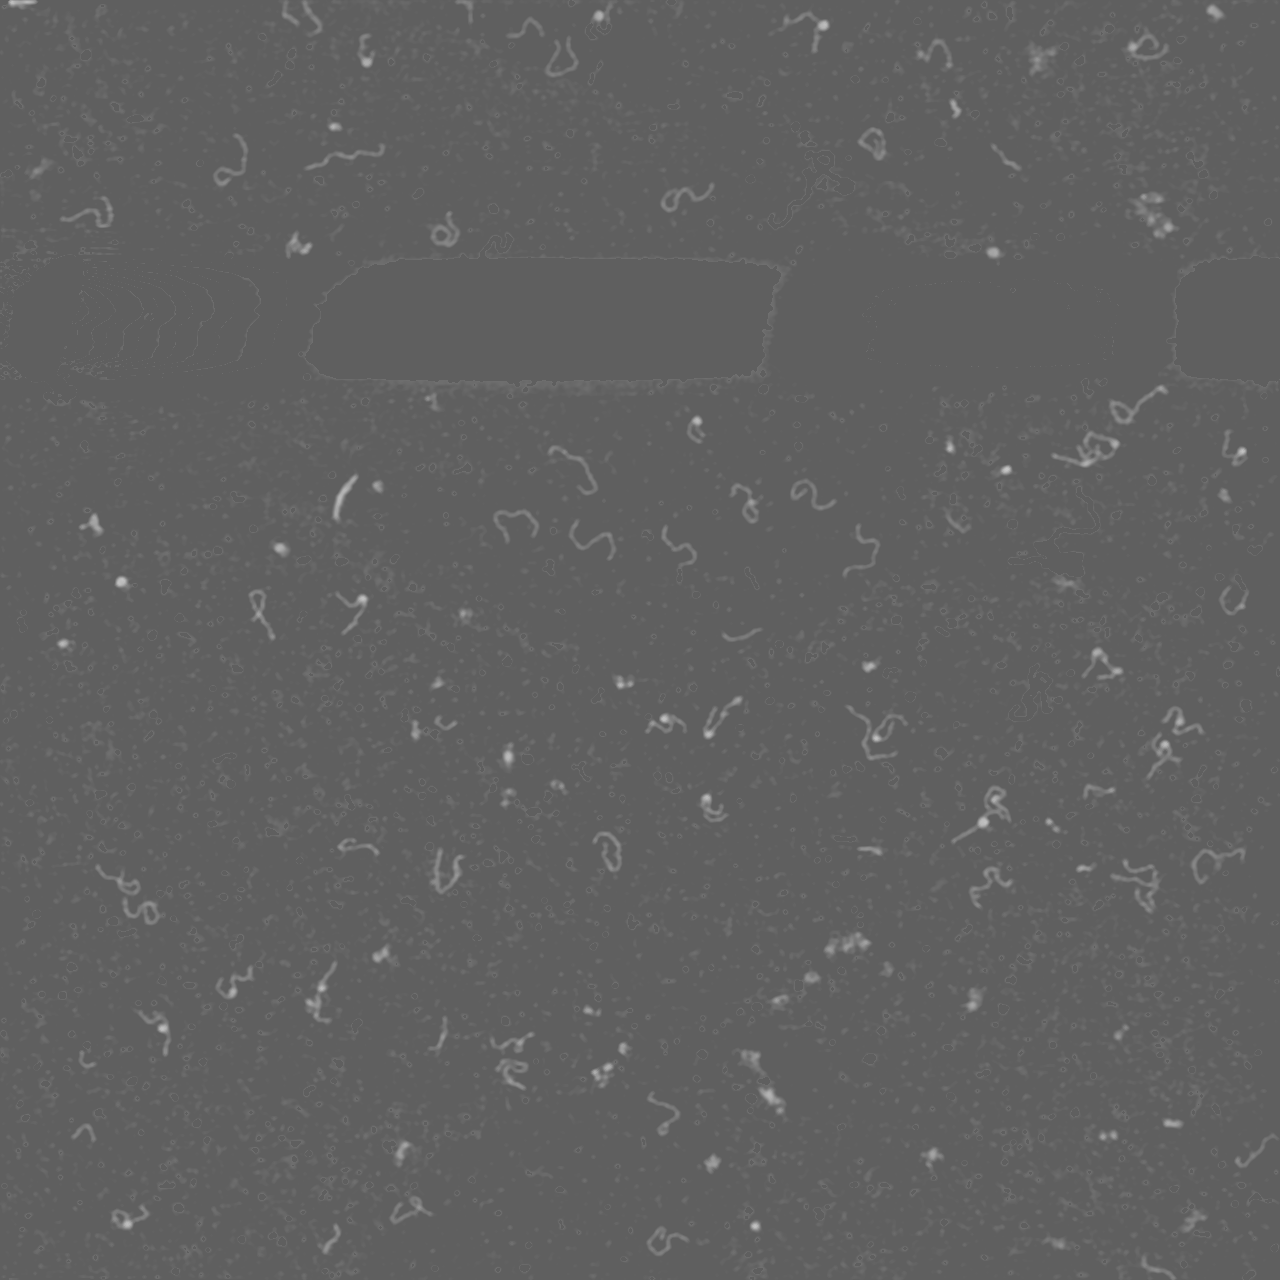
\includegraphics[width=\linewidth]{filtered.png}
		\caption{}
		\label{fig:filtered}
	\end{subfigure}%
	
	\caption{(a)Mask from binary image (b)Mask applied to original image}\label{fig:Process}
\end{figure}
This image is then used as a mask (compare Figure \ref{fig:mask}) which removes all non-DNA objects on the original image from step one.

This means subtract the detected regions on the mask from the original image and set them to the previous determined background level.
The result Figure \ref{fig:filtered} shows how the large outliers are removed and will therefore no longer contribute to the threshold in a negative way.
After this process a second threshold algorithm, in this case the moments threshold (see \ref{sec:Thresholding}), is applied to the original image. 
Duo to the previous steps the new calculated threshold is no longer influenced by background noise or polluted image regions.

In this case the new threshold is now at a intensity value of 111, compared to a intensity value of 135. Figure \ref{fig:compareThresh} shows the improvement in terms of recognized DNA objects on the sample image for type one noise as seen in Figure \ref{fig: Noise1}.
By using this approach it is now possible to analyze pictures with the first type of noise while they had to be discarded entirely before.


\begin{figure}[!htbp]
	\begin{subfigure}{0.5\textwidth}
		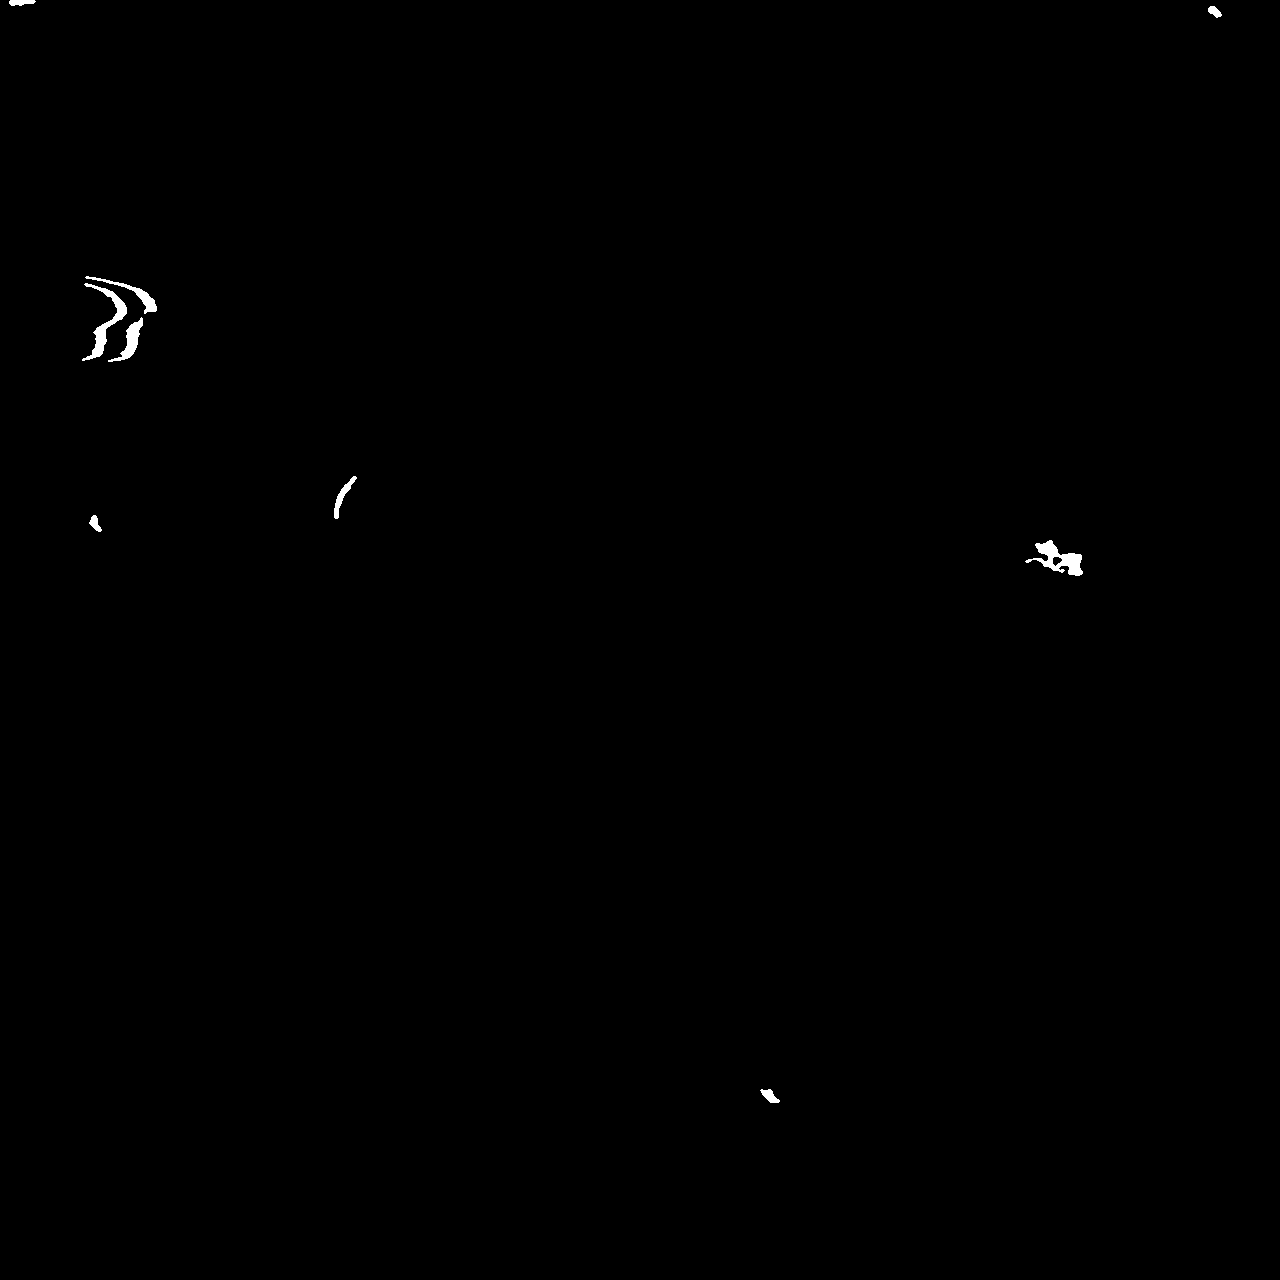
\includegraphics[width=\linewidth]{before.png}
		\caption{Before}
		\label{fig:bwbefore}
	\end{subfigure}%
	\hspace{\fill}
	\begin{subfigure}{0.5\textwidth}
		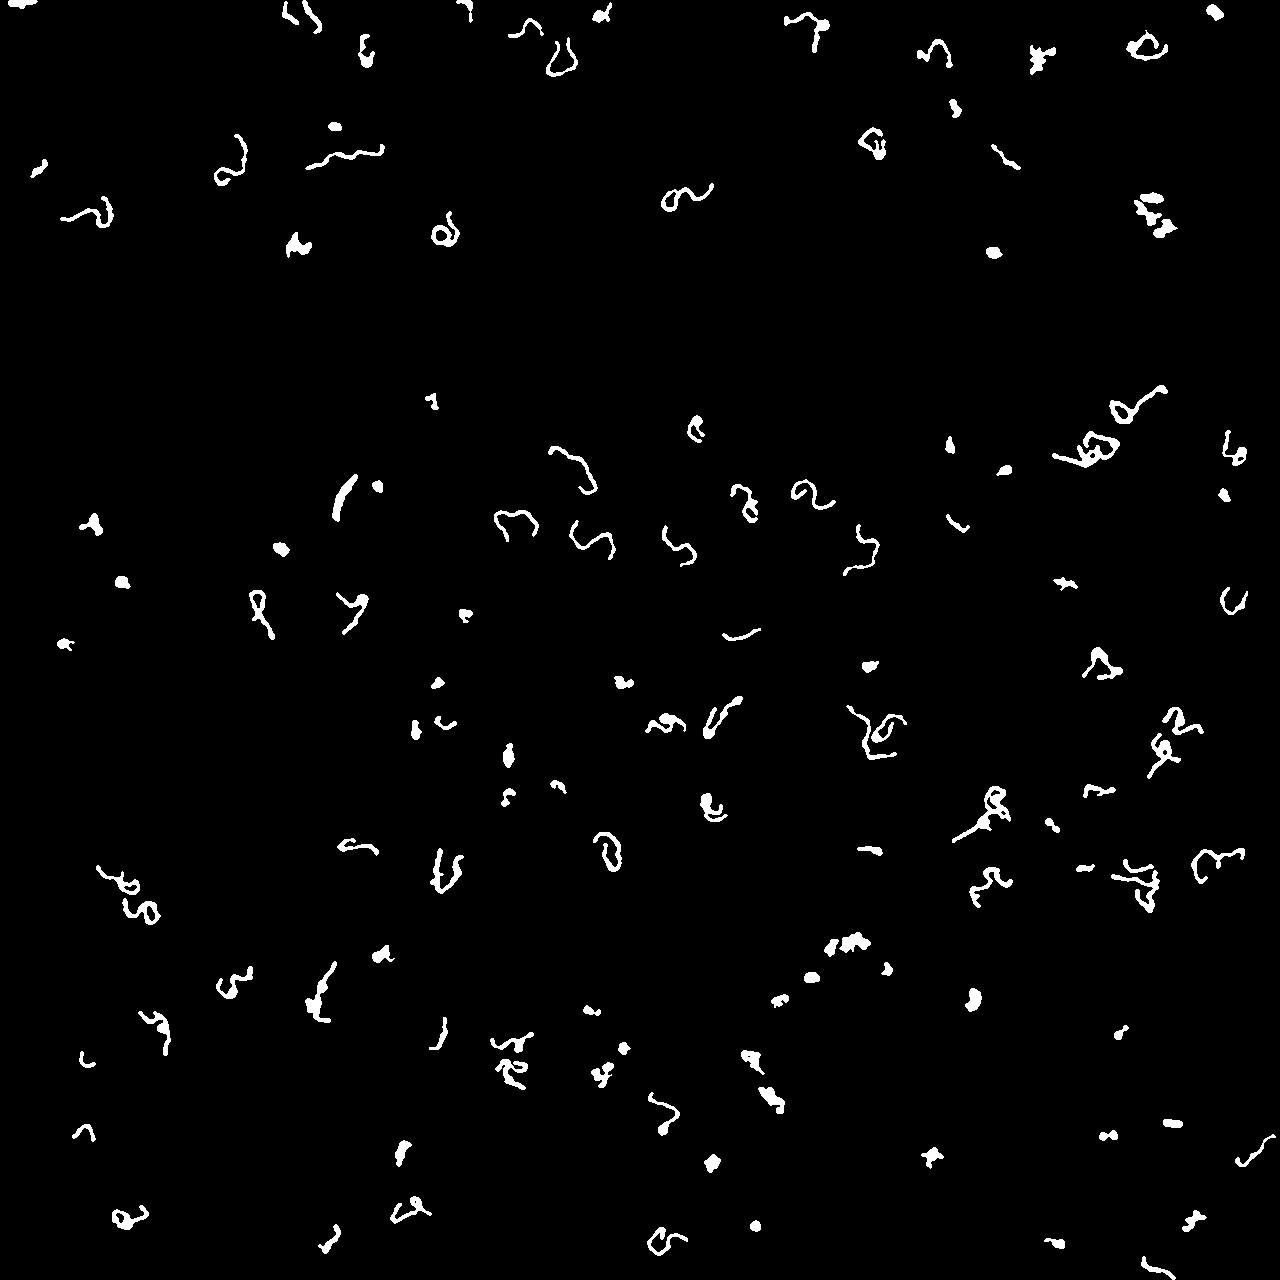
\includegraphics[width=\linewidth]{after.png}
		\caption{After}
		\label{fig:bwafter}
	\end{subfigure}%
	\caption{Comparison with previous method, noise type 1}\label{fig:compareThresh}
\end{figure}

\subsubsection{Limit Threshold}\label{sec: Limit Threshold}
The first two steps focused on keeping the noise and distribution of the height values in a tolerable range on image to image basis. The third and final step of this method aims at limiting the thresholds over the entire dataset.
For this technique a larger dataset of at least 50 images is required.
The histogram of all 105 test images shown in Figure \ref{fig:HistogramThresholds} shows that step one and two already improve the thresholds to a smaller range.
Also, only thresholds, which were too high, have been limited by these steps since only outliers in the upper value range have been treated, while lower values have been set to a fixed background.
The newly calculated thresholds are in a range between 0.4 and 0.46 which corresponds to pixel values of 102 and 117.
Looking at the images with the highest and lowest thresholds, it turns out that they are still prioritizing lower respectively higher pixel values. This results in too small DNA-strands or false positive detections.
In order to limit the probability of these cases the permissible range for thresholds is reduced even further. This is achieved by only allowing thresholds in the range of 1.5 times the standard deviation around the mean of the distribution.
The range is thereby limited to: 
\[
[\bar X - 1.5 * \sigma, \bar X + 1.5 * \sigma] 
\]
\[
= [0.4345-1.5*0.0129, 0.4345+1.5*0.0129] 
= [0.4152,0.4538]\,  % Formel allgemein hinzufügen
\]
All values outside of this interval are set to the nearest boundary.



\begin{figure}[!htb]
	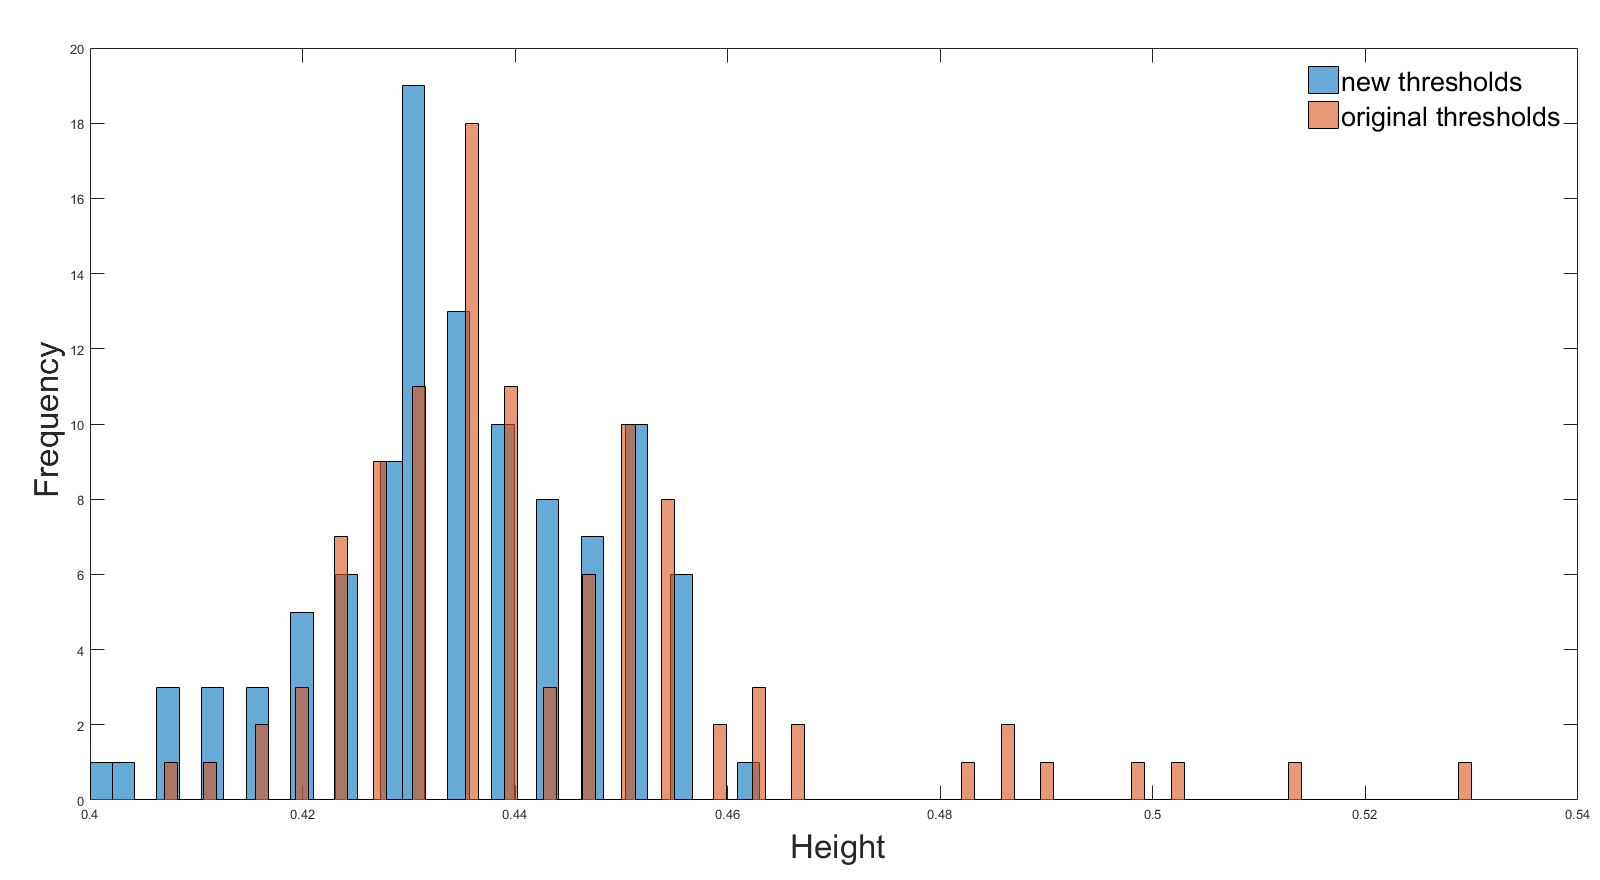
\includegraphics[width=1\linewidth]{thresholds.png}
	\caption{Threshold Distribution over the entire dataset (orange)before and (blue)after step one and two were applied}%formulierung ändern
	\label{fig:HistogramThresholds}
	\end{figure}
	As seen in Figure \ref{fig:compareThresh} this method effectively detects and removes polluted image regions and ensures a high DNA-strand detection on images with noise type one.
Due to the nature and height field of noise of type two this approach can only limit false detections to a certain degree (see Figure \ref{fig:compareThresh1}).
Although it was not expected to work on this kind of imperfections at all. While almost all DNA-strands are detected correctly some false positive still exist.
In conclusion, the proposed approach improves image quality and detection rate on very noisy images greatly while leaving already well processed images the way they are.

\begin{figure}[!htbp]
	\begin{subfigure}{0.5\textwidth}
		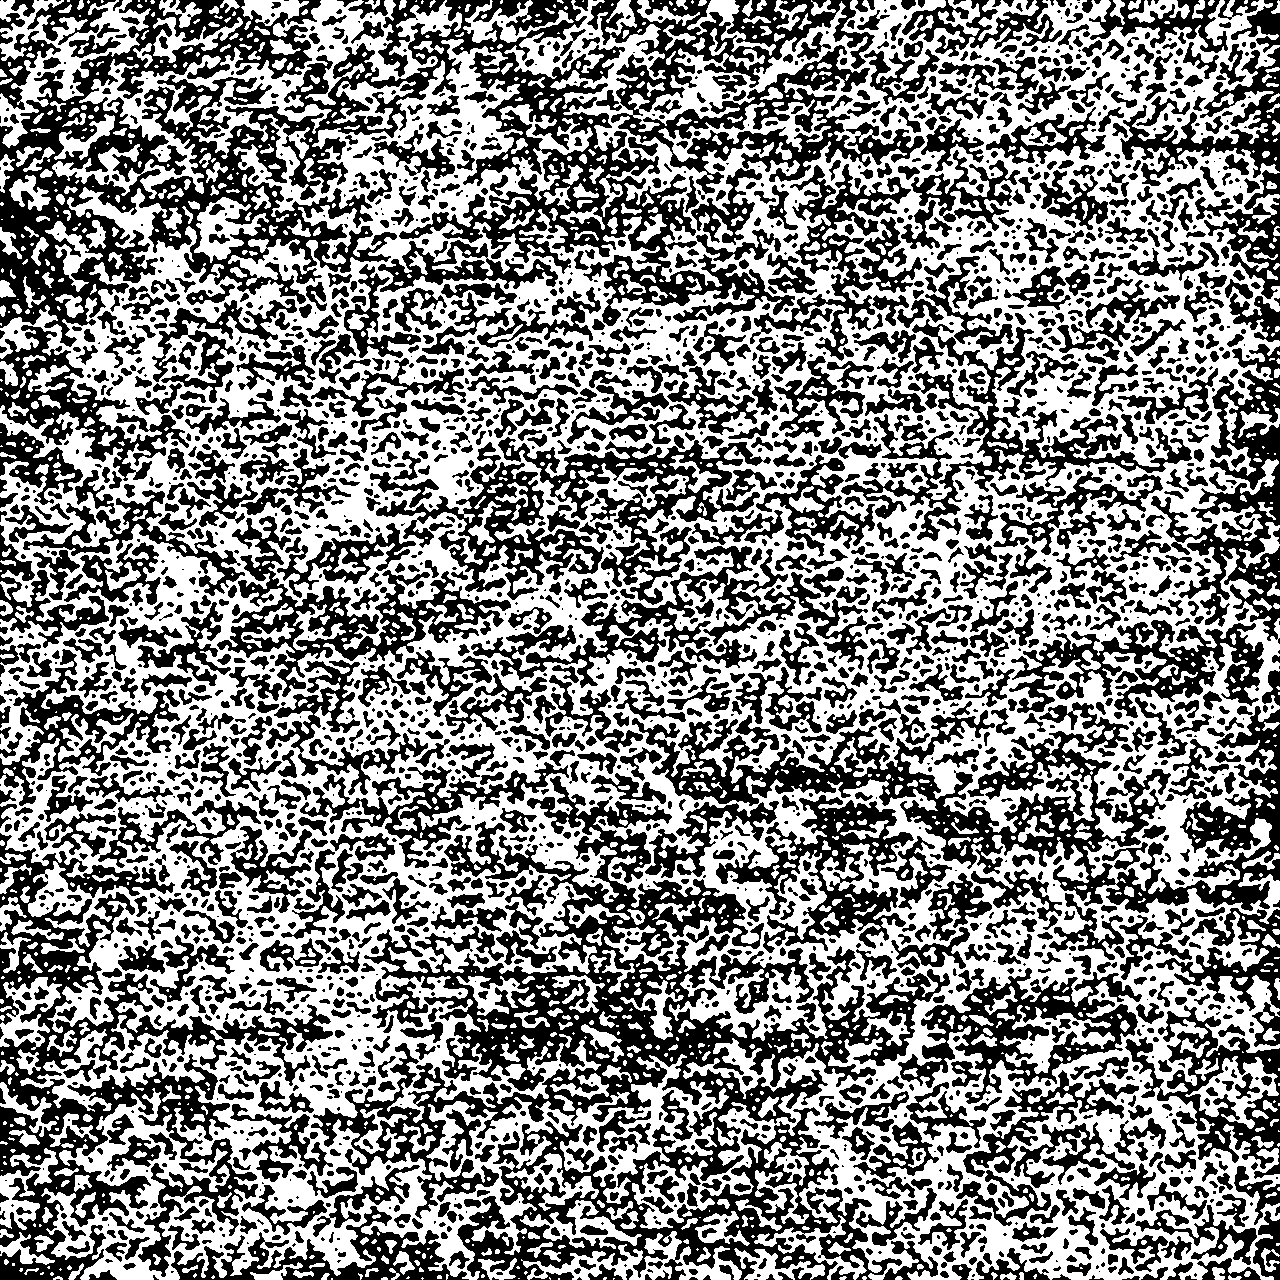
\includegraphics[width=\linewidth]{noise2before.png}
		\caption{Before}
		\label{fig:bwbefore}
	\end{subfigure}%
	\hspace{\fill}
	\begin{subfigure}{0.5\textwidth}
		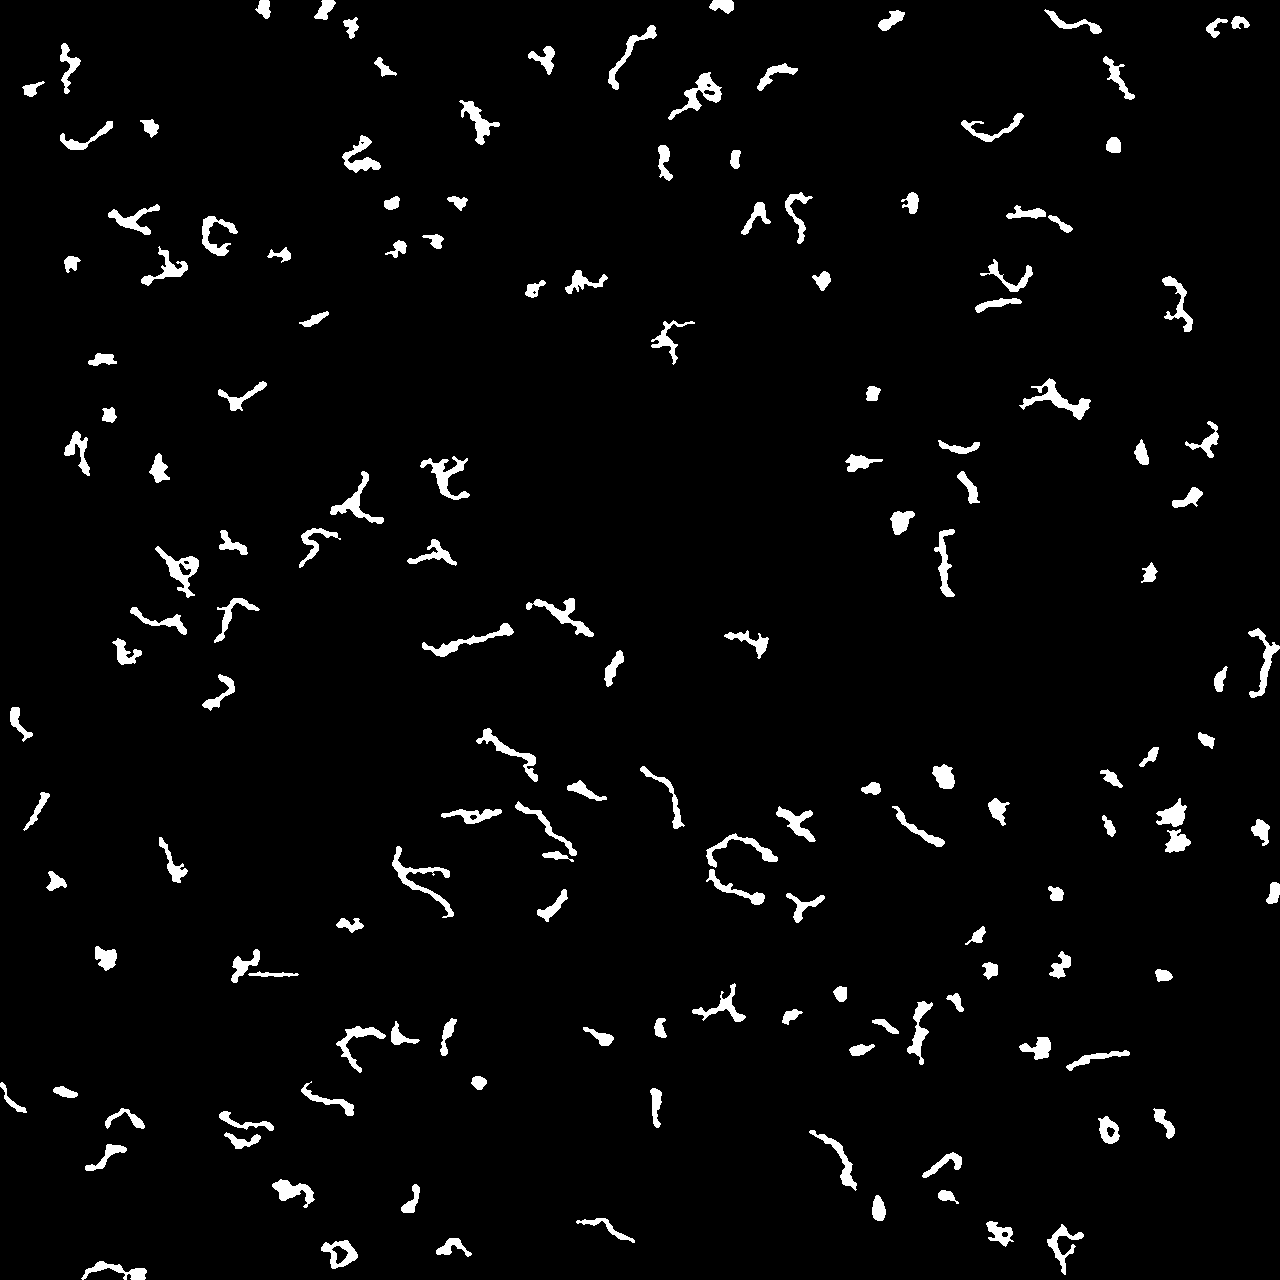
\includegraphics[width=\linewidth]{noise2after.png}
		\caption{After}
		\label{fig:bwafter}
	\end{subfigure}%
	\caption{Comparison with previous method, noise type 2}\label{fig:compareThresh1}
\end{figure}
\newpage

\subsection{Nucleosome Detection}\label{sec:Nucleosome Detection}
To determine whether the DNA contains a nucleosome and to measure the angle of the two branches wrapped around the nucleosome, an algorithm for nucleosome detection has been implemented. Due to the nucleosomes's appearance, an algorithm to detect bright circles with center $(i,j)$ and radius $r$, defined by
\begin{align}\label{eq: circle}
(x -i)^2+(y-j)^2 = r^2 
\end{align}
has been chosen, the MATLAB imfindcircles function. It is based on a Circular Hough Transform which provides robustness in the presence of noise, occlusion and varying illumination. Votes are cast in the Hough space which is made up of a cell for each pixel. Initially each cell is set to 0.

The algorithm considers foreground pixels that have a high image gradient value as candidates for the edges of a circle. For the image data in this project the foreground pixels are bright pixels. As the nucleosomes in the AFM images are blurry and of low contrast in relation to the background, their edges are weak and thus the image gradient threshold value has to be set relatively low. Each edge candidate pixel $p_{edge}=(x,y)$ is then the center point to a voting circle of a radius $r$, meaning that each edge candiate pixel casts votes in the Hough space to the bins $b = (i,j)$ which according to equation \ref{eq: circle} could be the center of the circle and therewith the center of the nucleosome.

The point where locally most voting circles coincide, which equals the bin in Hough space where votes accumulate, is marked as the center point of the actual circle, see Figure \ref{fig: houghTransfom1}. 

\begin{figure}[htb!]
\centering
\def\svgwidth{0.95\textwidth}
\input{houghTransfom1.pdf_tex}
\caption{Left: A voting circle (dashed) has its center point at a pixel of high gradient, e.g. on the actual circle's edge. Right: The actual circle that is to be detected (solid) is centered around the point where most voting circles meet.}\label{fig: houghTransfom1}
\end{figure}

However, the nucleosomes have different radii ranging between 4 and 6 pixels, such that the voting has to be done for several different radii leading to not just intersecting circles, but intersecting cones, see Figure \ref{fig: houghTransfom2}.

\begin{figure}[htb!]
\centering
\def\svgwidth{0.95\textwidth}
\input{houghTransfom2.pdf_tex}
\caption{Left: If the radius is unknown, votes will be cast not just to one circle but to many circles of radii $r$ in a given range.  Right: Voting circles of different radii add up to voting cones in Hough space.}\label{fig: houghTransfom2}
\end{figure}

As the image gradient direction is known, the problem is slimmed down to intersecting lines in the Hough space instead of the intersecting cones, see Figure \ref{fig: houghTransfom3}.
This is possible because the gradient direction tells the exact direction in which the center of the circle has to lie and subsequently one does not have to vote for a whole circle of possible center locations but just a single point or respectively for unknown radii, a line. The radius and circle center location is then given by the bin with the most votes, that is where most of the lines intersect.
%The corresponding radius is then estimated based on computing radial histograms. CHECK EXPLAIN

\begin{figure}[htb!]
\centering
\def\svgwidth{0.95\textwidth}
\input{houghTransfom3.pdf_tex}
\caption{Left: The image gradient gives information as to where the center of the actual circle is placed, hence votes are cast to just a point not to a circle. Right: Voting points for different radii add up to a voting line in Hough space.}\label{fig: houghTransfom3}
\end{figure}

 % [1] T.J Atherton, D.J. Kerbyson. "Size invariant circle detection." Image and Vision Computing. Volume 17, Number 11, 1999, pp. 795-803.
%[2] H.K Yuen, .J. Princen, J. Illingworth, and J. Kittler. "Comparative study of Hough transform methods for circle finding." Image and Vision Computing. Volume 8, Number 1, 1990, pp. 71–77.

%\begin{figure}[htb!]
%\centering
%\def\svgwidth{0.95\textwidth}
%\input{houghTransfom1.pdf_tex}
%\def\svgwidth{0.95\textwidth}
%\input{houghTransfom2.pdf_tex}
%\def\svgwidth{0.95\textwidth}
%\input{houghTransfom3.pdf_tex}
%\caption{\textbf{First row}: A voting circle (dashed) has its center point at a pixel of high gradient, therewith on the actual circle's edge. The actual circle that is to be detected (solid) is centered around the point in which most voting circles meet. \textbf{Second row}: If the radius is unknown, votes will be cast not just to one circle but many circles of radii $r$ in a given range.  Voting circles of different radii add up to voting cones in Hough space.\textbf{ Third row}: The gradient gives information as to where the center of the actual circle is placed, thus it is voted for a point instead of a circle. Right: Voting points for different radii add up to a voting line in Hough space.}\label{fig: houghTransfom}
%\end{figure}

Applying this method, the nucleosomes as well as noise of circular shape was detected. As only nucleosomes that are located on a DNA strand are of interest, the other detected circles can be dropped. This is done checking the pixel intensity value of the center points of all detected circles in the binary images. In those images noise is already deleted, such that the circles that were fitted to noise will have a pixel intensity value of zero at their center point. Thus, only circles with a non-zero pixel intensity value are considered as nucleosomes, see Figure \ref{fig: find nukleii}.

\begin{figure}[h!]
\includegraphics[width =0.5\textwidth]{findNukleii_rawCloseAn}
\includegraphics[width =0.5\textwidth]{findNukleii1_rawCloseAn}
\caption{Left: All detected nucleosomes are shown as red circles. Right: The detected nucleosomes after dropping those on overly big DNA strands (marked with black circles) and noise (marked with a white circle).} \label{fig: find nukleii}
\end{figure}
\newpage



\subsection{Thinning}\label{sec:Thinning} % sources: http://cgm.cs.mcgill.ca/~godfried/teaching/projects97/azar/skeleton.html, leelam
To obtain an accurate length measurement, the center line of the DNA is extracted. This is done by thinning the segmented DNA down to a single pixel width line corresponding to the skeleton of the DNA which can then be further processed for length and angle measurement. Two thinning algorithms have been tested in the scope of the project.



\subsubsection{Hilditch's Sequential Thinning}\label{sec:Hilditch's Sequential Thinning}
The first method is based on Hilditch's sequential thinning algorithm   \cite{lam1992thinning} and is implemented via MATLAB's \verb|bwmorph| function. For each DNA pixel $p$ the 8-neighborhood $N(p)$ is considered when deciding whether to disregard the pixel or keep it as part of the resulting skeleton. The neighborhood $N(p)$ includes the points $x_i, i= 1,\dots 8$ starting from the point east of pixel $p$ and counting upwards counterclockwise, compare Figure \ref{tab: neighborhood}. Their values correspond to the pixel intensity, such that
\begin{align*}
x_i = \begin{cases}
1 & \text{if } x_i \text{ is a DNA pixel}\\
0 & \text{if }x_i \text{ is a background pixel}
\end{cases}\, .
\end{align*}

\begin{figure}[htb]
\centering
\renewcommand{\arraystretch}{2}
\begin{tabular}{|c|c|c|}\hline
$x_4$ & $x_3$ & $x_2$ \\\hline
$x_5$ & $p$ & $x_1$ \\\hline
$x_6$ & $x_7$ & $x_8$\\\hline
\end{tabular}
\caption{8-Neighborhood of pixel $p$.}\label{tab: neighborhood}
\end{figure}

The pixels $p$ are scanned from left to right and top to bottom and are considered for deletion if they satisfy the following properties:
\begin{enumerate}
\item $p$ is a white pixel.
\item $p$ is not an isolated or end point
\item $p$ is a contour pixel, i.e., $p$ has at least one black 4-neighbor.
\end{enumerate}
For all those pixels, the algorithm performs two sub-iterations. In the sub-iterations pixel $p$ is deleted if the following conditions hold:
\begin{itemize}
\item \textbf{Condition 1} There is exactly one white connected component including white 4-neighbor pixels in $N(p)$:
\begin{equation*}
X_H(p)=1, 
\end{equation*}
where the crossing number $X_H(p)$ is the number of white connected components in $N(p)$:
\begin{align*}
& X_H(p) = \sum_{i=1}^4 b_i,\\\nonumber
& \text{where }
b_i=\begin{cases}
1 & \text{if } x_{2i-1} \wedge (\overline{x}_{2i} \vee \overline{x}_{2i+1})\\
0 & \text{else}
\end{cases} \\
\end{align*}
and where $x_i$ are the pixels in the neighborhood $N(p)$ as defined above and the pixel values are treated as boolean values such that $\overline{x}_i$ is the negation of $x_i$.
% DNA pixels are white, such that their value $x_i=1$, background pixels black and therewith $x_i = 0$. 

\item \textbf{Condition 2} Pixel $p$ is not an endpoint, branch point or isolated pixel and has to be a boundary pixel:
\begin{equation*}
2\leq \min\{n_1(p), n_2(p)\} \leq 3,
\end{equation*}
where
\begin{align*}
n_1(p) = \sum_{k=1}^4 \overline{x}_{2k-1}\vee \overline{x}_{2k}\\
n_2(p) = \sum_{k=1}^4 \overline{x}_{2k}\vee \overline{x}_{2k+1}
\end{align*}
\item \textbf{Condition 3} One pixel wide vertical and horizontal lines are not eroded by deletion of pixel $p$.
\begin{itemize}
\item First sub-iteration: $(x_2 \wedge x_3 \wedge \overline{x}_8) \vee x_1$
\item Second sub-iteration: $(x_6 \wedge x_7 \wedge \overline{x}_4) \vee x_5$
\end{itemize}
\end{itemize}
The two sub-iterations are repeated until the image stops changing. The result are one-pixel-wide ridges representing the center lines of the DNA strands, see Figure \ref{fig: thinning}. It can be observed that noise as well as the nucleosomes result in little branches on the center line. The branches are not needed for the calculation of the DNA's length such that they have to be removed, see Section \ref{sec:Erosion of Noise Branches}.

\begin{figure}[htb]
\centering
\includegraphics[width = 0.49\textwidth]{bin.png}
\includegraphics[width = 0.49\textwidth]{thinned.png}
\caption{Section of an AFM image after segmentation and binarization (left) and after thinning (right).}
\label{fig: thinning}
\end{figure}
\subsubsection{Zhang Suen Parallel Thinning}\label{sec:Zhang Suen Parallel Thinning}
The second method is the Zhang Suen thinning algorithm \cite{zhang1984fast} following the implementation given in \cite{linbo2013implementation}. It can be used to attenuate various types of digital patterns   \cite{widiarti2011comparing}.
Since it is a parallel method, the new value for any pixel can be computed using only the 8-neighborhood $N(p)$ values known from the previous iteration.
The contour pixels are deleted in two sub-iterations until no more changes occur in the image and a one-pixel wide 8-connected skeleton is obtained. A DNA pixel is deleted by setting its value to zero, the label of the background pixels.
Pixel $p$ is deleted, if the following conditions hold:
\begin{itemize}
\item \textbf{Condition 1} There is exactly one white connected component in $N(p)$:
\begin{align*}
A(p) = 1\, ,
\end{align*}
where $A(p)$ is the number of white to black crossings in the ordered set $x_1,x_2,\dots, x_8$ of $N(p)$.
\item \textbf{Condition 2} Pixel $p$ is not an endpoint or isolated pixel and has to be a boundary pixel:
\begin{equation*}
2 < n(p) < 6,
\end{equation*}
where $n(p)$ is the number of nonzero neighbors of $p$:
\begin{align*}
n(p) = \sum_{i=1}^8 x_i
\end{align*}
\item \textbf{Condition 3}
\begin{itemize}
\item First sub-iteration: Pixel $p$ is either a south-east boundary point or a north-west corner point. \begin{align*}
\overline{x}_1 \vee \overline{x}_7 \vee (\overline{x}_3  \wedge \overline{x}_5)
\end{align*}
\item Second sub-iteration: Pixel $p$ is either a north-west boundary point or a south-east corner point. \begin{align*}
\overline{x}_3 \vee \overline{x}_5 \vee (\overline{x}_1 \wedge \overline{x}_7)
\end{align*} 
\end{itemize}
\end{itemize}

The result of this algorithm differs from the result of Hilditch's algorithm as can be seen in Figure \ref{fig: thinnedHilditchZhang}. The center lines extracted with Hilditch's algorithm are smoother than the Zhang Suen algorithm. Further differences are discussed in Section \ref{sec: Results}.
\begin{figure}[htb!]
\centering
\includegraphics[width = 0.4\textwidth]{thinnedHilditch.png}
\includegraphics[width = 0.4\textwidth]{thinnedZhangSuen.png}
\caption{An AFM image section overlayed with the thinned DNA strands in white. Result of Hilditch's Sequential Thinning algorithm (left) and result of the Zhang Suen algorithm (right).}
\label{fig: thinnedHilditchZhang}
\end{figure}
\newpage
% second approach: Zhang-Suen https://github.com/linbojin/Skeletonization-by-Zhang-Suen-Thinning-Algorithm/blob/master/thinning.m

\subsection{Length Estimation}
At this stage of the program, each DNA object already has been isolated into a small black-and-white image that otherwise only contains this one DNA object, and both thinning algorithms have produced thinned DNA-strands. However, due to the nature of their operations, in most cases the resulting strands not only have two end points, but contain branches and multiple end points. Several examples can be seen in the right panel of Figure \ref{fig: thinning} above. In order to correctly determine DNA length, it is necessary to erode these branches so that afterwards only DNA strands without any branches and with only two ends are left. These will be called DNA backbones. Consequently, the next step in our routine is the erosion of these noise branches and the extraction of DNA backbones. \\

% Spline fitting
For Estimating the length of DNA fragments, several approaches seemed plausible. Firstly, backbone approximation by spline fitting was one prominent idea. For spline fitting, the DNA strand has to be subdivided into a few piecewise strands that add up into the original strand. Out of every piecewise strand some points are taken and these points are use to interpolate with a so called spline which is a polynom of n-th degree (n equals the number of supporting points minus 1). Normally these splines have to satisfy some more constraints to improve the accuracy and the smoothness of the interpolation. By interpolation of every substring it is possible to calculate the overall length of the object. The challenge of this method is to choose the best substrings and supporting points, and to perform these costly calculations without increasing the overall runtime too much. For these reasons, we decided not to follow this line.\\

% Pruning + freeman/Kulpa estimation
Another approach is to alter the DNA in a way that only one single strand remains and all side strands, which are most probably dirt or noise anyway, and some special points that are explained below are removed. After that the length of this single strand can be determined by simple length estimation algorithms as described by Rivetti \cite{rivetti2001accurate}. The most effort for this algorithm is altering the DNA string while the actual length estimation afterwards is rather easy. The huge advantage of this method is that by altering the DNA cases can be discovered in which the DNA forms a ring or overlaps with another DNA. Other length estimation algorithms have to take care about this separately. This is one of the methods used in our routine, and it is described in detail in Section \ref{sec:Iterative Length Estimation}.\\

An entirely different approach is described in Section \ref{sec:bfs_ssp_length_estimation}, however, which represents the other method used in our routine. Here, each thinned DNA fragment is converted into a graph object. On the basis of this, breadth-first-search and shortest path algorithms are used in order to extract the DNA backbone. After subsequent recovery of those pixels that were lost during the thinning process, length calculation is performed with help of the afore mentioned Kulpa Estimator.

\subsubsection{Algorithm D: Iterative length estimation}\label{sec:Iterative Length Estimation}

\paragraph{Problems of the data}
% Why do we need pruning?
\begin{figure}[H]
	\centering
	\begin{subfigure}[b]{0.36\textwidth}
		\includegraphics[width = \linewidth]{Lpoint.png}
		\caption{}
		\label{fig:lpoint}
	\end{subfigure}
	\hspace{\fill}
	\begin{subfigure}[b]{0.36\textwidth}
		\includegraphics[width = \linewidth]{Lpoint_mask.png}
		\caption{}
		\label{fig:lpoint_mask}
	\end{subfigure}
	\captionsetup{justification=centering}
	\caption{(a) one variant of a so called "L-point" \\(b) the four different submasks }
	\label{fig:lpoint_overview} % you need to include this to reference the figure afterwards
\end{figure}
In the dataset used for this algorithm often it occurs that the DNA strand is not one single strand but at some points sidebranches can be detected. This makes the length estimation much harder. Also L-points as shown in figure 
\ref{fig:lpoint} are a common problem since the algorithm has no distinct way to get from one of the outer pixels to the other outer one. In the proposed algorithm this can lead to problems where the parts of the DNA string are deleted that are not intended to or the object can be divided into multiple objects. Both effects are not desirable and are avoided by removing this critical L-points. \\
Another problem occurs when a branch is deleted. In some cases it can arise that a former branch point becomes an L-point after the deletion of the branch. In that case it has to be deleted, too, so the distinct way through the object is not destroyed again. So for every deleted branch there has also to be a routine that detects newly generated L-points.

% What is the problem with crossing DNA strings?
\begin{figure}[H]
	\centering
	\begin{subfigure}[b]{0.35\textwidth}
		\includegraphics[width=\linewidth]{praes2}
		\caption{}
		\label{fig: crossed}
	\end{subfigure}
	\hspace{20mm}
	\begin{subfigure}[b]{0.35\textwidth}
		\includegraphics[width=\linewidth]{rect4833}
		\caption{}
		\label{fig: ring}
	\end{subfigure}
	\captionsetup{justification=centering}
	\caption{(a) is a simple example for two overlapping strands\\ (b) DNA forming a ring}
	\label{fig: crossring} % you need to include this to reference the figure afterwards
\end{figure}
In figure \ref{fig: crossring} two special cases are shown. Case \ref{fig: crossed} shows a simple example for two overlapping DNA strands. Even though this is only an easy example in most cases where two DNAs overlap some kind of cross can be found. In case \ref{fig: ring} a DNA forming some kind of ring can be seen. This is mostly an error in the segmentation process or the DNA is intersecting with itself. All these cases can not be analyzed and are ignored in further processing steps. \\
For dealing with this two issues a special constraint is introduced. To better understand this constraint it is helpful to realize that a distinct DNA string has only two endpoints and no branchpoints (otherwise there would be a branch and therefore no distinct way through the object). Adding one additional branchpoint now automatically implies that there also has to be another endpoint. To be precise there has to be exactly one more endpoint because otherwise there would be a cross like in example \ref{fig: crossed} or a ring like in \ref{fig: ring} when the branchpoints produces no new endpoint. Secondly, it is important to notice that a ring like in figure \ref{fig: ring} has only one endpoint and one branchpoint. Creating a new endpoint would require another branchpoint too.\\
So what are the implications of these thoughts? Ultimately one will come to the conclusion that a good constraint to check for regular DNA strands is $\#endpoints - \#branchpoints = 2$. \\
This idea takes in regard that having a lower difference than 2 would imply to have more branchpoints and so some kind of ring in the DNA and having a higher difference would imply some kind of cross. \\
Of course this constraint will lead to the problem that some cases where noise is forming a cross or the DNA is a ring that could be analyzed anyhow will be thrown out. These cases are mostly DNAs that are in very noisy areas though and the accuracy of the length estimation for these strands would be low anyway. On the other hand it is a huge advantage to recognize molecules which are faulty and to make no false assumptions of their length. In that way statistics like the mean over all DNA strings are not influenced incorrectly. \\
In the course of the implementation another problem arised. What happens if the cross- and ring structure combine in a way that adds up in a constraint of 2 nonetheless (imagine a ring and two additional intersections)? This problem was eliminated by only looking if a cross occurs. Further explanation can be found later. The case of a DNA forming a ring is still treated by checking with the constraint.\\
Eventually this method has found a good middle ground between evaluating as many molecules as possible and throwing out DNA one can not analyze in a reliable way.

\paragraph{Description of the proposed method}
Firstly, the algorithm asserts that the image is not empty. This is just a step of precaution but should be done in every good code nonetheless. If the image is empty a length of 0 is returned and the algorithms immediately terminates.\\
To avoid border cases of points lying at the edge of the image the image is padded with a single row of zeros. Afterwards essential information is extracted out of the image like width, height and the connected components of the object. Reextracting the connected components is necessary since by padding the pixel indices are shifted.\\
The next important step is to create an adjacency matrix of the pixels of the connected component. An adjacency matrix essentially describes for each pixel which other pixels can be reached from this one. In image processing this refers most often to neighbouring pixels in a 8-neighbourhood. If the reader is not familiar with adjacency matrices reading of further papers is strongly recommended. It should be mentioned that it is sufficient to create the matrix by using only the pixels that are part of the object which are stored in a pixel index list and it is not needed to create a adjacency matrix using all image pixels. \\
A speciality of the proposed method is that the adjacency matrix does not only represent the neighbourhood but also the direction in which the neighbour lies (see fig \ref{fig: example_adj}).\\
The next step is to remove all L-points. L-points are described earlier in this section. The removal is performed by iterating over all object pixels that have exactly two neighbourgs. Points with less neighbours are endpoints and pixels with more neighbours branchpoints. Therefore a 3x3 clipping around the current pixel is cut out and the clipping again subdivided into 4 quadrants (see fig \ref{fig:lpoint_mask}). A pixel is now identified as an L-point if the point is considered an L-point in one of the quadrants (see red quadrant in fig \ref{fig:lpoint_mask}). L-points are deleted from the picture as well as the adjacency matrix.\\

\begin{figure}[H]
	\centering
	\begin{subfigure}[b]{0.3\textwidth}
		\includegraphics[width=\linewidth]{neighborhood}
		\caption{}
		\label{fig: example_neighborhood}
	\end{subfigure}
	\\
	\begin{subfigure}[b]{0.3\textwidth}
		\includegraphics[width=\linewidth]{example}
		\caption{}
		\label{fig: example_strand}
	\end{subfigure}
	\hspace{\fill}
	\begin{subfigure}[b]{0.1\textwidth}
		\includegraphics[width=\linewidth]{example_idlist}
		\caption{}
		\label{fig: example_idxlist}
	\end{subfigure}
	\hspace{\fill}
	\begin{subfigure}[b]{0.33\textwidth}
		\includegraphics[width=\linewidth]{example_adj}
		\caption{}
		\label{fig: example_adj}
	\end{subfigure}
	\captionsetup{justification=centering}
	\caption{(a) numeration of the neighborhood (b) simple example of thinned strand (c) index list of the image (d) resulting adjacency list \\
		Note that the adjacency list is symmetric only with opposing cases }
	\label{fig: adj_example} % you need to include this to reference the figure afterwards
\end{figure}

%% Dennis Philip 02.08
At this point the branchpoints and endpoints are computed with
\begin{verbatim}
bwmorph(picture, 'branchpoints') 
bwmorph(picture, 'endpoints') 
\end{verbatim}
respectively. As described before, the segmented strand is tested on its validity by the constraint of $\#endpoints - \#branchpoints = 2$. If a branchpoint now has exactly 4 neighbours, it is assumed to be a self-intersection which is reliable for the sequential Hilditch-Thinning but not for the algorithm by Zhang Suen. Further explanation and discussion of the results can be found in Sections \ref{sec:Hilditch's Sequential Thinning} and \ref{sec:Zhang Suen Parallel Thinning}. \\

\begin{figure}[H]
	\centering
	\begin{subfigure}[b]{0.32\textwidth}
		\includegraphics[width=\linewidth]{remove1}
		\caption{}
		\label{fig:remove1DenPhi}
	\end{subfigure}
	\begin{subfigure}[b]{0.32\textwidth}
		\includegraphics[width=\linewidth]{remove2}
		\caption{}
		\label{fig:remove2DenPhi}
	\end{subfigure}
	\begin{subfigure}[b]{0.32\textwidth}
		\includegraphics[width=\linewidth]{remove3}
		\caption{}
		\label{fig:remove3DenPhi}
	\end{subfigure}
	\captionsetup{justification=centering}
	\caption{(a) DNA string with the selected branchpoint (green), another branchpoint (red) and the nearest endpoint (blue) to the green point\\(b) incorrect deletion of a substring (c) correct deletion}
	\label{fig:removalsDenPhi} % you need to include this to reference the figure afterwards
\end{figure}

For every valid object the algorithm now iterates over the list of branchpoints until it is empty. With each loop an arbitrary single branch point will be extracted from the mask provided by bwmorph. Using bwdistgeodesic with this singular branchpoint mask, a distance estimation towards each endpoint is calculated. The function is only used in this case since it has no option to calculate the length with more precise estimators (like the Kulpa estimator proposed by \cite{rivetti2001accurate}) but is reliable enough to give an idea which endpoint is nearest to the current branchpoint that is critical in this step. Removing all pixels of this shortest branch should in theory be rather easy but may lead to unwanted problems. For example a strand with another branchpoint between the used branchpoint and the closest endpoint would result in two separate objects. In figure \ref{fig:removalsDenPhi} a correct and incorrect removal of a substring can be seen.\\
To avoid this, only the pixels from the endpoint to the \textit{closest} branchpoint are removed. For this the adjacency matrix is of great help since it provides the neighbouring pixels. After deleting a point from the image, it has to be deleted from the image as well as the adjacency matrix. \\
Another, yet unlikely, case would happen if two endpoints are of exactly the same distance from the branchpoints. Should bwdistgeodesic indeed return two valid endpoints, only the first element of the array is selected to avoid critical errors. \\
At the end of each iteration step the branchpoint and endpoint matrices are updated as well. It is crucial that in the branchpoint mask the deleted branchpoint is altered and not necessarily the one which was initially selected by the algorithm. Also note that the branchpoint is \textit{not} removed from the image but only from the branchpoint mask.
The initial branch will still be deleted in a later iteration step either way, so the order doesn't impact it in any negative way but can prevent critical cases as shown. \\

\begin{figure}[H]
	\centering
	\begin{subfigure}[b]{0.32\textwidth}
		\includegraphics[width=\linewidth]{critical1}
		\caption{}
		\label{fig:critical1DenPhi}
	\end{subfigure}
	\begin{subfigure}[b]{0.32\textwidth}
		\includegraphics[width=\linewidth]{critical2}
		\caption{}
		\label{fig:critical2DenPhi}
	\end{subfigure}
	\begin{subfigure}[b]{0.32\textwidth}
		\includegraphics[width=\linewidth]{critical3}
		\caption{}
		\label{fig:critical3DenPhi}
	\end{subfigure}
	\captionsetup{justification=centering}
	\caption{(a) original DNA string (b) without L-point removal (c) with L-point removal}
	\label{fig:criticalDenPhi} % you need to include this to reference the figure afterwards
\end{figure}

Another problem that showed up during initial testing was that the algorithm sometimes didn't fully remove a certain branch, or so it seemed. This was the result of the branchpoint, after removing the shortest branch, could transform into an L-point. To avoid such behaviour, and assert a singular and unique path from end to end, it has to be checked whether the branchpoint fulfills the L-point criteria mentioned earlier in this chapter. In figure \ref{fig:criticalDenPhi} the problem is visualized. Note how the purple point in \ref{fig:critical2DenPhi} would lead to a non-unique path.\\
With this step the processing of the strand has been almost completed. If there have been no problems up to this point, the strand seems to be a valid object and is therefore treated as such. In the case that one of the earlier mentioned abortion criteria terminated the algorithm, the dnaObject is then marked as invalid by setting the isValid flag of the object class to 0. \\
%% Dennis 03.08
The following steps are similiar to the algorithm described in Sections \ref{sec:PixelRecovery} and \ref{sec:Length Estimation}, and have only been slightly altered. The method is only described here for sake of completeness. 
\\
To improve the quality of the final estimate it should also be considered to reestimate the border regions of the strand. With the thinning algorithms, especially the region around the endpoints is usually eroded from each direction which leads to an overall shorter strand in thinned form. Various approaches have already been proposed as already described in Section \ref{intro_length_determination}. Based on the endpoints and their respective neighbouring pixels, a reestimation direction is established by taking a vector in this direction (see figure). By overlaying the original fragment with the thinned one it can now be determined whether there is another pixel in the estimation direction that belongs to the fragment. The process is repeated until it meets a pixel which is no longer part of the fragment or the image boundary is reached. \\
The last step in the algorithm is then to calculate the partial length of each fragment, so long as they do have exactly one attached nucleosome. For this a boolean function parameter called dnaHasNucleos was introduced which lets the algorithm decide whether there are any nucleosomes attached at all. The exact number of attached nucleosomes can be referenced by the object's value 'attachedNucleo'. \\
For these valid objects the length of each partial strand (divided by the nucleosome) is stored which results in an array of length two. \\
For fragments without any nucleosomes, or more than one attached, the fragment length is stored as one single value.
The final length calculation is done by using the Kulpa estimator which provides a more accurate estimate than the classic Freeman estimator \cite{rivetti2001accurate} for certain DNA lengths. \\
For both formulas the neighborhood of the pixel is considered: Either the pixels are evenly aligned or are adjoining diagonally. By multiplying the number of each cases with a respective factor a final length can be calculated. \\

Freeman estimator: $ 1 * \#EvenPixels + \sqrt{2} * \#OddPixels$ \\
Kulpa estimator: $0.948 * \#EvenPixels + 1.343 * \#OddPixels$ \\

For this purpse the following subroutine was introduced to calculate the final length:
\begin{verbatim}
calcKulpaLength(IndexList, ThinnedImage)
\end{verbatim}
For calculating subsegment-length, this function is simply called twice with the respective partial strand. \\
The matrix indices of the pixels are split into row and column indices. Following the introduced neighborhood model, a evenly aligned pixel-pair would either have the same row or column indices. By simply substracting the difference of neighboring index-pairs it is possible to accumulate the total number of evenly aligned pixels. The number of odd pixels is easily calculated by substracting the evenly number from the total amount of pixels belonging to the strand. As a last step the length is determined by the aforementioned formula. An example is shown in figure \ref{fig:partialLengthDenPhi}.

\begin{figure}[H]
	\centering
	\begin{subfigure}[b]{0.34\textwidth}
		\includegraphics[width=\linewidth]{ghostbusters1}
		\caption{}
		\label{fig:partialLengthDenPhi1}
	\end{subfigure}
	\hspace{5mm}
	\begin{subfigure}[b]{0.34\textwidth}
		\includegraphics[width=\linewidth]{ghostbusters2}
		\caption{}
		\label{fig:partialLengthDenPhi2}
	\end{subfigure}
	\captionsetup{justification=centering}
	\caption{An example strand with a nucleosome}
	\label{fig:partialLengthDenPhi} % you need to include this to reference the figure afterwards
\end{figure}
\newpage
\paragraph{Results}
\begin{figure}[H]
	\centering
	\begin{subfigure}[b]{0.32\textwidth}
		\includegraphics[width=\linewidth]{preprocessed}
		\caption{}
		\label{fig:preprocImageLength}
	\end{subfigure}
	\hspace{5mm}
	\begin{subfigure}[b]{0.32\textwidth}
		\includegraphics[width=\linewidth]{processed}
		\caption{}
		\label{fig:pastprocImageLength}
	\end{subfigure}
	\captionsetup{justification=centering}
	\caption{(a) DNA string before processing (b) DNA strand after processing}
	\label{fig:LengthsThingiesReference} % you need to include this to reference the figure afterwards
\end{figure}

In figure \ref{fig:LengthsThingiesReference} one can see the strand before and after the before mentioned algorithm processed it. One can clearly see that the L-Point in the upper left corner is removed as well as the two branches in the middle of the string. These results can be reproduced with any valid string of DNA, even if it is more complex. One can conclude that the first goal of the algorithm, which was essentially the pruning of the strand and the removal of the L-points, is working as intended. \\
\\
The length estimation itself returns reasonable lengths and the general calculated range of the analysed DNA strands is accurate. However, one problem of the Kulpa estimator is that it was originally developed to analyze DNA strands with a length of more than 600 base pairs \cite{rivetti2001accurate}. The DNA in the used data set has a length of about 660 base pairs. While the Kulpa should be rather accurate for this cases it seems that the length of the DNA is a bit too short for this method and as a result the Kulpa estimator deviates from the original lengths. An exact analysis of this can be found in chapter (reference).
\\
Overall the Kulpa estimator proved to be more stable than the Freeman estimator and for regular cases (no outliers) the deviation was significantly smaller. To be exact the deviation of the Freeman estimator was at least four percent while the Kulpa estimator only deviated by about one percent. 
\\
Another goal of the method was to sort out as many invalid DNA strings as possible. With the introduced constraint and the sorting out of DNA strands that have an intersection this aim was achieved and the amount of false positives could be greatly reduced. A disadvantage of this is that some valid DNA is discarded. The advantage of having the security that the result is comparable in its entirety is favourable though. Otherwise deductions like the mean would be influenced by false positives and, therefore, less reliable.
\\
A disadvantage of the algorithm is that the subroutine for determining the partial lengths was originally designed for algorithm C (see \ref{sec:bfs_ssp_length_estimation}) and the embedding in this code was harder than it seemed at first. Since the implementation did not return satisfying results a comparison is not possible at this point. 

\newpage
\subsubsection{Algorithm C: Erosion using Breadth-First-Search and Shortest Path Algorithms} \label{sec:bfs_ssp_length_estimation}
Basis of this method are the conversion of DNA objects into graphs and subsequent usage of graph algorithms for branch removal. It consists of the following steps:
\begin{enumerate}
	\item Exclusion of invalid DNA objects
	\item Conversion of pixel lists to graph representations
	\item Determination of the two most distant end points
	\item Determination of shortest path between those end points
\end{enumerate}
Invalid DNA objects are those that meet any of the following criteria:
\begin{itemize}
	\item Self-intersecting: The length of an DNA strand that intersects itself cannot be meaningfully determined.
	\item Wrong size: Since the size of all DNA strands that have been used in the preparation of the AFM probe is known, any detected DNA object can be expected to be in size range of 40 to 150 pixel. If it contains less pixels, it either has been truncated during preparation of the AFM probe or it is no DNA at all. If it is made up from more pixels it either is an artifact that has not been deleted during filtering and thresholding, or it is made up from several overlapping DNA strands. 
\end{itemize}
In all of these cases, length determination does not make sense. Such objects are marked as being invalid and are excluded from further processing.
\begin{figure}[htb!]
	\centering
	\includegraphics[width = 0.2\textwidth]{dna_with_loop.png}
	\caption{Self-intersecting DNA object. The Euler number of this black-and-white image is 0, indicating that there is at least one object with one hole in the image.}
	\label{fig:dna_with_loop}
\end{figure}
\\Self-intersection of an DNA object means that the DNA is looping back on itself and then touches or crosses itself (compare Figure \ref{fig:dna_with_loop}). A consequence of this is that the DNA object can be considered to be an object with a hole. This, in turn, means that the topology of this object is different compared to an object that does not have a hole, which is reflected in the Euler number of its image. Therefore, for each DNA object the Euler number is calculated using the MATLAB function \textit{bweuler}. It returns the number of objects in an image minus the number of holes. Since for each DNA object an image exists that only contains this one object, this function efficiently can be used to distinguish between self-intersecting and non-intersecting DNA objects. If the Euler number is 0, then an object with an hole has been detected, and the DNA object is flagged as being invalid. Only if the Euler number is 1, the DNA object will be further processed.\\

\paragraph{Conversion of DNA fragments into graph objects}

\begin{figure}[!htbp]
	\centering
	\begin{subfigure}{0.25\textwidth}
		\includegraphics[width=\linewidth]{small_DNA_obj.png}
		\caption{Exemplary black-and-white image of a small DNA object}
		\label{fig:dna_obj_example}
	\end{subfigure}
	\begin{subfigure}{0.25\textwidth}
		\includegraphics[width=\linewidth]{small_DNA_obj_adj_matrix.png}
		\caption{Corresponding upper triangular adjacency matrix}
		\label{fig:dna_obj_adjMatrix}
	\end{subfigure}
	\begin{subfigure}{0.25\textwidth}
		\includegraphics[width=\linewidth]{small_DNA_obj_graph.png}
		\caption{Undirected graph}
		\label{fig:dna_obj_graph}
	\end{subfigure}
	\caption{Simple example for the conversion of DNA objects to undirected graphs.
		(a) From a small image containing exactly one DNA object, (b) an upper triangular adjacency matrix is created where all ones (red) represent edges between directly neighboring pixels. Only pixels containing information, i.e. white pixels, need to be considered and here, no pixel is neighbor to itself. (c) Such a matrix represents an undirected graph.}
	\label{fig:dna_graph_creation}
\end{figure}
The next step is the conversion of DNA fragments to graph objects. This approach relies on the fact that, at this stage of the entire process, the so far detected and thinned DNA objects internally are represented as chains of white pixels that belong to exactly one object. Since thinning already has taken place, this approach assumes that any pixel in such a chain is only neighbor to other pixels that represent other links of the chain.\\
Therefore, each DNA object can be transformed into a graph G (Figure \ref{fig:dna_graph_creation}). The nodes of this graph are those pixels representing the DNA object, while the graph's edges describe the direct 8-neighborhood between pixels (Figure \ref{fig:dna_obj_adjMatrix}). Since in this case neighborhood between pixels is a bijection, the resulting graph G is undirected, and it suffices to create G from an upper triangular adjacency matrix.\\
\begin{figure}[htb!]
	\centering
	\begin{subfigure}{0.22\textwidth}
		\includegraphics[width=\linewidth]{small_DNA_graph_bfs1.png}			
		
		\vspace{0.2cm}
		
		\includegraphics[width=\linewidth]{small_DNA_obj_bfs1.png}
		\caption{First bfs}
		\label{fig:dna_graph_bfs1}
	\end{subfigure}
	\begin{subfigure}{0.22\textwidth}
		\includegraphics[width=\linewidth]{small_DNA_graph_bfs2.png}
		
		\vspace{0.2cm}
		
		\includegraphics[width=\linewidth]{small_DNA_obj_bfs2.png}
		\caption{Second bfs}
		\label{fig:dna_graph_bfs2}
	\end{subfigure}
	\begin{subfigure}{0.22\textwidth}
		\includegraphics[width=\linewidth]{small_DNA_graph_ssp.png}	
		
		\vspace{0.2cm}
		
		\includegraphics[width=\linewidth]{small_DNA_obj_ssp.png}
		\caption{Shortest path }
		\label{fig:dna_graph_ssp}
	\end{subfigure}
	\begin{subfigure}{0.22\textwidth}
		\includegraphics[width=\linewidth]{small_DNA_real_bfs.png}
		
		\vspace{0.2cm}
		
		\includegraphics[width=\linewidth]{small_DNA_real_ssp.png}
		\caption{Example DNA}
		\label{fig:dna_real_ssp}
	\end{subfigure}
	\caption{Determining DNA backbones via two breadth-first searches (bfs) and a shortest path search.
		(a) On the graph G representing a DNA object, one iteration of breadth-first search (bfs) with a randomly chosen start node (green) will return one node (red) of the pair of nodes that is connected via the longest path within G. (b) Using this node as starting node (green) in a second iteration of bfs will return the other node (red) of this pair. (c) Calculating the shortest path between these two nodes returns the DNA backbone (green edges) while excluding noise branches (red edge). The upper row of panels (a) to (c) depicts results on the graph object introduced in Figure \ref{fig:dna_graph_creation}, the lower row shows the same results in the respective DNA object representation. (d) A thinned DNA object as detected by the program is shown. The upper image indicates the pair of nodes furthest apart from each other, the lower image highlights the shortest path between them (green), a noise branch (red) and pixel that were lost during the thinning process (blue).}
	\label{fig:dna_backbone_detection}
\end{figure}
Having created a graph representation for each DNA object, another simple measure allows for the detection of further invalid DNA objects. At this stage of the program, a valid DNA object is expected to be a single DNA strand without any intersections. Its graph will be a tree, i.e. a graph in which each pair of nodes is connected via exactly one, and only one path. However, if smaller DNA strands intersect each other without fully forming any circle, they appear to be one large object that still can be within the size limits. Although a graph of such an object also will be a tree, this tree will have a high branching factor, which means that the difference between the number of edges and the number of nodes is larger compared to a valid DNA object as described above. Therefore, any DNA object whose graph representation does not fulfill the following criteria is also excluded from further processing and flagged as being invalid.
\begin{center}\textit{number of edges - number of nodes $\leq$ 2}\end{center}

\paragraph{Erosion of Noise Branches}\label{sec:Erosion of Noise Branches}
Due to their graph representations, it is now possible to determine exactly those end points of the DNA objects that are the furthest apart (see Figure \ref{fig:dna_backbone_detection}). This is equivalent to determining each graph's diameter, i.e. the largest distance between any two connected nodes of a graph. It can be achieved by successively performing two breadth-first searches (bfs) on G. MATLAB already provides such a functionality (\textit{bfsearch}) that is optimised for MATLAB internal graph objects. Therefore, we specifically converted DNA objects into MATLAB graph objects. For the first bfs (compare Figure \ref{fig:dna_graph_bfs1}), a start node is chosen randomly. Due to the nature of this algorithm, the last node to be discovered can only be a node that has the largest distance to the starting node. If there are several nodes with the same largest distance, which of these is discovered last depends on the implementation of the bfs algorithm. Because all of them are equally far apart from the start node, any of these nodes is considered a correct result.\\
This node, however, can then be used as start node in the second run of bfs (compare Figure \ref{fig:dna_graph_bfs2}). Since bfs will again return the node with the largest distance to the start node last, we now know the exact pair of nodes that are furthest apart from each other in G.\\
This information next is used to find the shortest path between these two nodes in G (see Figure \ref{fig:dna_graph_ssp}). Also here an optimized implementation provided by MATLAB was used, \textit{graphshortestpath}. Since all graphs are undirected with uniform edge weights of 1, a shortest path algorithm specifically designed for this type of graph was used that has an overall time complexity of O(N+E), with N being the number of nodes and E being the number of edges.
The resulting paths represent DNA backbones excluding noise branches, since for a shortest path between two nodes it holds that it connects its two extremal nodes (start and target node) in G via a path that cannot be shortened without severing the connection between both nodes.

\paragraph{Recovery of lost pixels}\label{sec:PixelRecovery}
Having determined the true DNA backbones, it next is necessary to restore pixels that have been lost from the DNA fragments during the thinning process and that are essential for length determination. Such pixels are those that lay at the end of an DNA fragment, as can be seen in the upper image of Figure \ref{fig:end_pixel_recovery4}. This loss cannot be avoided since both tested thinning algorithms cannot differenciate between pixels that are part of the end of a fragment and pixels that constitute some other part of the DNA fragment. 

\begin{figure}[htb!]
	\centering
	\begin{subfigure}{0.25\textwidth}
		\includegraphics[width=\linewidth]{thin_DNA_1.png}
		
		\vspace{0.2cm}
		
		\includegraphics[width=\linewidth]{thick_DNA_1.png}
		\caption{Initial state}
		\label{fig:end_pixel_recovery1}
	\end{subfigure}
	\begin{subfigure}{0.25\textwidth}
		\includegraphics[width=\linewidth]{thin_DNA_2.png}
		
		\vspace{0.2cm}
		
		\includegraphics[width=\linewidth]{thick_DNA_2.png}
		\caption{First iteration}
		\label{fig:end_pixel_recovery2}
	\end{subfigure}
	\begin{subfigure}{0.25\textwidth}
		\includegraphics[width=\linewidth]{thin_DNA_4.png}
		
		\vspace{0.2cm}
		
		\includegraphics[width=\linewidth]{thick_DNA_4.png}
		\caption{Second iteration}
		\label{fig:end_pixel_recovery3}
	\end{subfigure}
	\begin{subfigure}{0.20\textwidth}
		\includegraphics[width=\linewidth]{thick_thin_before_recovery.png}
		
		\vspace{0.2cm}
		
		\includegraphics[width=\linewidth]{thin_after_recovery.png}
		\caption{Result}
		\label{fig:end_pixel_recovery4}
	\end{subfigure}
	\caption{Recovery procedure for pixels lost during DNA thinning.\\
		The upper row shows a thinned DNA fragment's end, the lower row the respective DNA's state before thinning. (a) After determination of the DNA backbone, those pixels that were lost from the fragment's ends during the thinning process need to be recovered. One of those ends is schematically depicted. (b) In the first iteration, a direction is derived from the last two pixels of one end. The thick DNA image is used as reference to find lost pixels. (c) In the second iteration, the newly discovered pixel is used to determine whether another pixel needs to be recovered. (d) The upper image shows an overlay of thin and thick DNA, clearly indicating that pixels were lost. The lower image shows the same DNA strand after pixel recovery. 
	}
	\label{fig:end_pixel_recovery}
\end{figure}

An useful and easy to implement approach already has been indicated in Section \ref{sec:IntroPixelRestoring}. Each DNA backbone only has two ends by definition. So, for each of a DNA backbone's end, consider the last two pixels as depicted in the upper panel of Figure \ref{fig:end_pixel_recovery2}. The relation of those two pixels towards each other within the 8-neighborhood of the end pixel of the two identifies an unambiguous position at which a pixel possibly could have been lost. The information whether a pixel has been lost or not can easily be retrieved by comparing the pixel at this position with the pixel at the same position in the image of the not-yet-thinned DNA fragment (see Figure \ref{fig:end_pixel_recovery2}, lower panel). If the pixel at that position is part of the DNA fragment, it has to be restored, and can now be considered to be the new end point of this DNA fragment end. This process is repeated until no pixel can be restored anymore. At this point, the DNA backbone is complete, and its length can be computed.


\paragraph{Length Estimation}\label{sec:Length Estimation}
Length computation generally is done as has already been described in Section \ref{intro_length_determination}. Because Rivetti and Codeluppi \cite{rivetti2001accurate} showed that the Kulpa Estimator has higher accuracy than the Freeman Estimator, is easy to implement and has only low impact on the overall runtime, we decided to use this measure for DNA fragment length calculation, as well.\\
Length estimation has to be done differently for DNA fragments with and without nucleosome, respectively. For a DNA fragment without nucleosome, simply its entire DNA backbone needs to be considered. In the case of an DNA fragment with nucleosome, however, the DNA backbone has to be divided into exactly those two parts that point away from the nucleosome, i.e. the nucleosome's both arms. 
\begin{figure}[htb!]
	\centering
	\includegraphics[width = 0.5\textwidth]{length_calc_two_arms.png}
	\caption{Intersection between the DNA backbone and the nucleosome of its DNA fragment.\\
		Dark green pixels represent the not-yet-thinned DNA fragment with its bound nucleosome, and its DNA backbone is represented by white and light-green pixels. The nucleosome, as it was detected by the program, is shown in red.}
	\label{fig: length_calc_two_arms}
\end{figure}
This can be achieved by using the same method that is used during angle measurement (compare Section \ref{sec:Angle Measurement}). Intersections of the DNA backbone with the circle (red) which is defined by the radius of the nucleosome is calculated as visualized in Figure \ref{fig: length_calc_two_arms}. Then, those parts of the backbone that are inside this circle are temporarily deleted (light green pixels), which results in only two arms remaining (white pixels). For each of these arms, now, the length is calculated similarly as it is done for the entire backbone in case of free DNA fragments. In the unlikely case that an intersection between the detected nucleus and the DNA backbone cannot be computed, no length will be determined.


\subsection{Angle Measurement}\label{sec:Angle Measurement}
For the DNA strands with a nucleosome, the angle between the two DNA branches is measured. DNA strands with more than one nucleosome will not be assigned an angle measurement neither will DNA strands without nucleosome. Furthermore, if the nucleosome is positioned at the end of the DNA strand as depicted in Figure \ref{fig: angle not}, the angle cannot be measured either. 
\begin{figure}[htb]
\includegraphics[width = 0.49\textwidth]{angle_endstrand.png}
\includegraphics[width = 0.49\textwidth]{angle_two.png}
\caption{DNA strand with the nucleosome on the strand end (left) and more than one detected nucleosome (right). These cases are not considered for angle measurement.}\label{fig: angle not}
\end{figure}

To discard those cases a mask is set up which is zero at all pixels belonging to the nucleosome and one elsewhere. Multiplication of the mask with the image of the DNA's center line, that is the thinned DNA after erosion of all branches, leads to an image of the DNA branches. After applying a connected component analysis each branch is represented by one connected component. All samples with a number of connected components unequal to two will be dropped and only the remaining samples with two connected components, respectively branches, are considered for the angle measurement.
Two ways to measure the angle between the two branches of the DNA have been implemented in the scope of this project.

\subsubsection{Measurement over Nucleosome Center}\label{sec:Measurement over Nucleosome Center}
The first method for the angle measurement is to determine the intersection of the DNA branches and the circle fitted to the nucleosome, draw one line from each intersecting point to the nucleosome center and then calculate the angle between those two lines. This approach has been described in \cite{bussiek2005dna}.
To determine the intersection of the DNA branches with the circle fitted to the nucleosome, for both branches the Euclidean distance of each of its pixels to the DNA's nucleosome center $c$ is measured. The pixel with the smallest distance $d$ equals the intersecting pixel points $p$ of this branch.
The angle $\theta$ between the two lines connecting the intersecting points $p_1$ and $p_2$ with the nucleosome center $c$ is calculated by
\begin{align}
\theta &= \arccos{\frac{a\cdot b}{||a||||b||}}\, ,\label{eq: angle}\\
\text{where } a &= c-p_1 \text{ and } b = c-p_2 \, .\nonumber
\end{align}

However, it turned out that the resulting angles are in many cases not representative for the actual branch angles, see Figure \ref{fig: angle1}. 
\begin{figure}[htb!]
\centering
\def\svgwidth{0.5\textwidth}
\input{angle_1.pdf_tex}
\caption{The angle $\theta=\theta_1 = 108^{\circ}$ between the two DNA branches measured with method 1.}\label{fig: angle1}
\end{figure}
\subsubsection{Measurement over Fitted Lines}\label{sec:Measurement over Fitted Lines}
The second method for the angle measurement follows \cite{kepert2003conformation} fitting a line to the first part of a few micrometers of each branch and calculates the angle between those two fitted lines.
The first step is to select the pixels belonging to the first part of the two branches. 

Let \begin{align*}
r_{max} = r+s\, ,
\end{align*}
where $r$ is the nucleosome radius, estimated in Section \ref{sec:Nucleosome Detection} and $s$ is the value determining the size of the first part. A mask which is zero outside of a circle of radius $r_{max}$ around the nucleosome center is applied to the image of the DNA branches leading to the pruned DNA branch stumps.

  Again a connected component analysis is performed on the pixel set, returning two pixel sets, each representing one of the two branch stumps.
The next step is to fit one line to each branch. This is done by computing a least squares polynomial of order one for the given branch points, returning a slope $m$ and an offset $t$ for each branch line.
Subsequently the angle between the two lines is calculated according to Equation (\ref{eq: angle}), which requires the intersecting point $c = [c_x\, c_y]^{\top}$ of the two fitted lines given by:
\begin{align*}
c_x &= -\frac{t_1-t_2}{m_1-m_2}\\
c_y &= m_1 c_x + t_1 = m_2 c_x + t_2\, .
\end{align*}

\begin{figure}[htb!]
\centering
\def\svgwidth{0.5\textwidth}
\input{angle_2.pdf_tex}
\caption{The angle $\theta=\theta_2 = 170^{\circ}$ between the two DNA branches measured with method 2.}\label{fig: angle2}
\end{figure}
%a least squares polynomial 


\subsection{Optimization}\label{sec:Optimization}
\section{Results}\label{sec: Results}
\subsection{Validation}\label{sec:Validation}
\subsection{Biological Significance}\label{sec: Biological Significance}
\section{Discussion}\label{sec: Discussion}
\section{Conclusion and Outlook}\label{sec: Conclusion and Outlook}

\newpage
\bibliography{sources}
\bibliographystyle{unsrt}

\end{document}
